\section{A brief review of the Penrose process}
\subsection{The Kerr spacetime}
\subsection{The Reissner-N\"ordstrom spacetime}

\section{Majumdar-Papapetrou Spacetimme}

In this section we will show that energy can be extracted from the MP spacetime using the Penrose process. Since the MP spacetime consists of a binary of Reissner-N\"ordstrom constituents, we will use an electrically charged particle to extract electromagnetic energy from the system.

\subsection{Spacetime metric}

For two black holes of masses $M_1$ and $M_2$ and electric charges $Q_1 = M_1$ and $Q_2 = M_2$, in equilibrium and separated by a distance $2a$ along the $z$-axis, the MP line element, in Weyl's cylindrical coordinates, is given by~\cite{SMERAK2016}

\begin{equation}
  \ud s^2 = -U(\rho,z)^{-2} \ud t^2 + U(\rho,z)^2\left[\ud\rho^2 + \rho^2\ud\phi^2 + \ud z^2\right],
  \label{ch:penrose_binaries/ch:penrose_binaries/eq:majumdar_papapetrou_line_element}
\end{equation}
%
where
\begin{equation}
  U(\rho,z) = 1 + \frac{M_1}{\sqrt{\rho^2 + (z+a)^2}} + \frac{M_2}{\sqrt{\rho^2 + (z-a)^2}}.
  \label{ch:penrose_binaries/eq:mp_metric_potential_cylindric}
\end{equation}

The components of the electromagnetic potential $\tens{A}{}{\mu}$ associated with the MP solution are

\begin{equation}
  \tens{A}{}{\mu} = \left(1 - \frac{1}{U}\right)\tens{\delta}{}{\mu t},
  \label{ch:penrose_binaries/eq:electromagnetic_potential_mp}
\end{equation}
%
where $\tens{\delta}{}{\mu\nu}$ is the Kronecker delta.

We remark that Weyl's coordinates describe only the exterior of the black holes, in such a way that their event horizons and their interiors are collapsed into the points $\rho=0, \, z=\pm a$. In particular, due to its staticity, the MP spacetime does not possess an ergosphere (in the usual sense of a spacetime region outside the event horizon where it is impossible for freely-falling particles to ``stand still" -- i.e remain static -- while still being able to escape to infinity). In view of that, and motivated by the possibility of Penrose processes for single charged black holes, instead of analysing geodesic motion we will start by studying the trajectories of charged particles in the MP spacetime.

\subsection{Motion of charged particles}

The motion of a massive charged test particle (with charge-to-mass ratio $\mu$) in any given spacetime with metric $g_{\mu \nu}$ and electromagnetic potential $\tens{A}{}{\mu}$ is governed by the Lagrangian
\begin{equation}
  \mathcal{L} = \frac{1}{2}\mtrtens{\mu}{\nu}\tens{\dot{x}}{\mu}{}\tens{\dot{x}}{\nu}{} - \mu \tens{A}{}{\alpha}\tens{\dot{x}}{\alpha}{},
  \label{ch:penrose_binaries/eq:lagrangian_for_charged_particle}
\end{equation}
%
where $\tens{x}{\mu}{} = \tens{x}{\mu}{}(\lambda) =  \left(t(\lambda), \rho(\lambda), \phi(\lambda), z(\lambda)\right)$ denotes the particle's position (parametrized by its proper time $\lambda$) and dots represent derivatives with respect to $\lambda$. Taking into account the explicit form of the MP metric and of the MP electromagnetic potential, the Lagrangian \eqref{ch:penrose_binaries/eq:lagrangian_for_charged_particle} can be recast as~\cite{RYZNER2015}

\begin{equation}
  \mathcal{L} = \frac{1}{2}\left[-\frac{\dot{t}^2}{U^2} + U^2\left( \dot{\rho}^2 + \rho^2\dot{\phi}^2 + \dot{z}^2 \right) \right] - \mu\left(1-\frac{1}{U}\right)\dot{t}.
  \label{ch:penrose_binaries/eq:explicit_lagrangian_for_charged_particle}
\end{equation}
%
Since the expression above does not depend explicitly on the coordinates $t$ and $\phi$, two constants of motion can be identified, namely the energy divided by the mass of the particle (as measured by a freely-falling observer at infinity),

\begin{equation}
  E \equiv -\del{\mathcal{L}}{\dot{t}} = \frac{\dot{t}}{U^2} + \mu\left(1-\frac{1}{U}\right),
  \label{ch:penrose_binaries/eq:conserved_energy}
\end{equation}
%
and the angular momentum about the $z$ axis divided by the mass of the particle (as measured by a freely-falling observer at infinity),

\begin{equation}
  L \equiv \del{\mathcal{L}}{\dot{\phi}} = U^2 \rho^2 \dot{\phi}.
  \label{ch:penrose_binaries/eq:conserved_momentum}
\end{equation}

Plugging these constants of motion into the 4-velocity normalization condition, $\tens{\dot{x}}{\mu}{}\tens{\dot{x}}{}{\mu} = -1$, and solving for the energy $E$, yields

\begin{equation}
  E = \mu\left(1-\frac{1}{U}\right) + \sqrt{\frac{L^2}{\rho^2U^4} + \frac{1}{U^2} + \dot{\rho}^2 + \dot{z}^2}
  \label{ch:penrose_binaries/eq:alternative_expression_for_energy},
\end{equation}
where the negative root has been neglected due to the fact that $E$ must be positive at infinity when $\mu = 0$ (for a detailed discussion about positive and negative root states for $E$ see Ref. \cite{RUFFINI1971}). We note that Eq.~\eqref{ch:penrose_binaries/eq:alternative_expression_for_energy} reduces to the expression found in Ref.~\cite{DENARDO1973} for a Reissner-Norstr{\"o}m black hole if the mass of one of the black holes is taken to be zero and an appropriate coordinate system, centered around the other black hole, is used.

Finally, the equations of motion are obtained directly from the Euler-Lagrange equations. After using \myref{ch:penrose_binaries/eq:conserved_energy} and \myref{ch:penrose_binaries/eq:conserved_momentum} to eliminate $\dot{t}$ and $\dot{\phi}$ from the resulting expressions, one is left with

\begin{multline}
  \ddot{\rho}-\frac{L^2(U+\rho\indexdel{\rho}U)}{\rho^3 U^5} + \frac{2\dot{\rho}\dot{z}\indexdel{z}U - (E^2 + \dot{z}^2 - \dot{\rho}^2)\indexdel{\rho}U}{U} \\- \frac{\mu}{U}\left(\mu-2E+\frac{E-\mu}{U}\right)\indexdel{\rho}U = 0,
  \label{ch:penrose_binaries/eq:ode_for_rho_motion}
\end{multline}
%
and
\begin{multline}
  \ddot{z}-\frac{L^2\indexdel{z}U}{\rho^2 U^5} + \frac{2\dot{\rho}\dot{z}\indexdel{\rho}U - (E^2 - \dot{z}^2 + \dot{\rho}^2)\indexdel{z}U}{U} \\- \frac{\mu}{U}\left(\mu-2E+\frac{E-\mu}{U}\right)\indexdel{z}U = 0,
  \label{ch:penrose_binaries/eq:ode_for_z_motion}
\end{multline}
which reduce to the equations of motion found in Ref.~\cite{ASSUMPCAO2018} for neutral particles. Together with Eqs.~\eqref{ch:penrose_binaries/eq:conserved_energy} and \eqref{ch:penrose_binaries/eq:conserved_momentum}, the two equations above fully determine the trajectory of a massive charged particle in the MP spacetime once appropriate initial conditions have been specified.

\subsection{Generalized ergosphere}

The possibility of extracting energy from a black hole through the Penrose mechanism is intimately linked to the existence of negative-energy trajectories (as measured by observers far away from the black hole). As explained before, in the MP spacetime (and in other static spacetimes like Reissner-Nordstrom) there are no ergospheres in the usual sense, meaning that geodesic motion is always associated with positive energy trajectories. Any charged particle moving through the MP spacetime, however, will be affected by Lorentz forces from its electromagnetic interaction with the black holes and, consequently, will satisfy the equations of motion derived in the previous section. Even though there are no ergospheres in MP, since the trajectories associated with Eqs.~\eqref{ch:penrose_binaries/eq:conserved_energy}, \eqref{ch:penrose_binaries/eq:conserved_momentum}, \eqref{ch:penrose_binaries/eq:ode_for_rho_motion} and \eqref{ch:penrose_binaries/eq:ode_for_z_motion} are not geodesics, negative values for the constant of motion $E$ are not forbidden \emph{a priori}. If negative energy trajectories exist in the MP spacetime, then one can define generalized ergospheres as the regions of spacetime where they are allowed to exist. The concept of generalized ergospheres is not new, however, and was first introduced by Denardo and Ruffini for the Reissner - Nordstr\"om solution in Ref.~\cite{DENARDO1973}, where they have additionally shown that the Penrose process is viable in this spacetime by presenting concrete examples. That being said, defining a generalized ergosphere for the MP spacetime is a natural step forward from D. and R. since it consists of two extremely charged RN black holes.

From Eq.~\eqref{ch:penrose_binaries/eq:alternative_expression_for_energy} it is evident that, for fixed $\mu$, the energy is completely determined by the angular momentum $L$, and the values of $\rho$, $z$, $\dot{\rho}$ and $\dot{z}$  at any given instant of time. Therefore, at a fixed position in space, the minimum possible energy is associated with particles at rest. Letting $\dot{\rho}=\dot{z}=0$ and $L=0$ (i.e.~$\dot{\phi}=0$), we conclude that the minimum energy $E_{\mathrm{min}}$ for a particle, as a function of its position, is
\begin{equation} \label{ch:penrose_binaries/eq:minimum_energy}
  E_{\mathrm{min}} = \mu\left(1-\frac{1}{U}\right) + \frac{1}{U}.
\end{equation}

By requiring the minimum energy to be negative, we find that $\mu$ must necessarily be negative (which means that the particle's charge is opposite to the charge of the black holes) and that the particle (at rest) must be inside the spatial region determined by
\begin{equation} \label{ch:penrose_binaries/eq:negative_energy_condition}
  \frac{M_1}{\sqrt{\rho^2 + (z+a)^2}} + \frac{M_2}{\sqrt{\rho^2 + (z-a)^2}} > - \frac{1}{\mu}.
\end{equation}

Since $\mu$ is a dimensionless quantity, it makes sense to recast the left side of \eqref{ch:penrose_binaries/eq:negative_energy_condition} as a dimensionless quantity as well so that we are comparing two pure numbers. To do so, one must simply divide both numerators and denominators of the left side of the inequality by, say, $M_1$ and define $\overline{\rho} \equiv \rho/M1$, $\overline{z} \equiv z/M1$, $M \equiv M_1/M_2$, $\alpha = a/M1$ to obtain

\begin{equation} \label{ch:penrose_binaries/eq:rescaled_negative_energy_condition}
  \frac{1}{\sqrt{\overline{\rho}^2 + (\overline{z}+\alpha)^2}} + \frac{M^{-1}}{\sqrt{\overline{\rho}^2 + (\overline{z}-\alpha)^2}} > - \frac{1}{\mu}.
\end{equation}

This last inequality determines the generalized ergosphere of the MP spacetime as a region depending only on three dimensionless parameters: $M$, $\alpha$ and $\mu$. Particles with charge-to-mass ratio $\mu$ inside the region determined by \eqref{ch:penrose_binaries/eq:rescaled_negative_energy_condition} can have negative energies, while particle outside will never have negative energies. Note that this notion of ergosphere depends not only on the geometry of the spacetime, but also on properties of the particle.

In order to have a graphical representation of the generalized ergosphere, let us use cartesian-like coordinates, also reescaled by $M_1$, $(\overline{x},\overline{y},\overline{z})$ related to Weyl's coordinates by $\overline{x}=\overline{\rho} \cos \phi$ and $\overline{y}=\overline{\rho} \sin \phi$. In Figs.~\ref{ch:penrose_binaries/fig:splitting_1}-\ref{ch:penrose_binaries/fig:splitting_4}, we plot the generalized ergosphere for a MP black hole binary of unitary mass-ratio $M$, whose horizons (represented by red dots) have also unitary separation parameter $\alpha$. As the value of $\mu$ increases, one can observe that the generalized ergosphere splits into two disconnected spherical regions with the same (albeit smaller than the original) radius. Thus we see that the bigger the value of $\mu$, the closer to the horizon an orbit must be in order to realize energy extraction. Extrapolating this result makes it easy to see that the maximum possible amount of energy can only be extracted if a particle is orbiting exactly \emph{at} the event horizon. We will explore this fact further in another section of this work but this result is in agreement with~\cite{RUFFINI1971}.

In Figs.~\ref{ch:penrose_binaries/fig:mass_increase_1}-\ref{ch:penrose_binaries/fig:mass_increase_2}, we turn to the influence of the mass-ratio in the generalized ergosphere's shape while keeping fixed $\mu = -1$ and $\alpha = 1$. The ergosphere starts of with the same shape as in Fig.~\ref{ch:penrose_binaries/fig:splitting_1}. As the mass-ratio increases, the ergosphere around one of the black holes is enlarged while the other's shrunken until a split-up occurs, and again, one ends up with two disconnected regions but this time of different sizes, the larger of which is centered around the heavier black hole. Again, this is to be expected. Because the MP solution represents extremally charged black holes, as the mas of the objects increase (or decrease) so does their electric charge thus allowing for more energy to be extracted and consequently a larger generalized ergosphere.

Finally, in Figs.~\ref{ch:penrose_binaries/fig:distance_1}-\ref{ch:penrose_binaries/fig:distance_2} we show the effects on the generalized ergosphere resulting from the increase in the distance parameter $\alpha$ with $M=1$ and $\mu=-1$ fixed. Initially the ergosphere is shaped as in Fig.~\ref{ch:penrose_binaries/fig:splitting_1}. Yet again, as the value of $\alpha$ increases, the ergosphere becomes elongated along the $z$ direction, assuming a `peanut'-like shape until it is split into two disconnected regions. From \eqref{ch:penrose_binaries/eq:rescaled_negative_energy_condition}, we can verify that the splitting occurs when $\alpha = -(M^{-1}+1)\mu$. If the black holes are moved further apart, the system will eventually behave as two isolated extremal black holes of mass $M$, each one surrounded by its own spherical generalized ergosphere.

It's also very important to point out that for small separations the generalized ergosphere of the binary system becomes equal to the one around a single RN black hole of mass $M_1 + M_2$. One can easily see that by taking the limit $a \rightarrow 0$ in \eqref{ch:penrose_binaries/eq:negative_energy_condition} and going to spherical coordinates, related to Weyl's coordinates trough $\rho = \sin\theta$ and $z=r\cos\theta$, which leads to the conclusion that that the generalized ergosphere is the spherical region centered around the origin which satisfies $r < -\mu (M_1 + M_2).$ This is precisely the same region as the one presented in Eq. (12) of Ref.~\cite{DENARDO1973} if one considers an extremal black hole in coordinates such that the event horizon is a point at the origin (which amounts the transformation $r \rightarrow r + M$) with the RN solution's mass parameter $M$ replaced by the total mass of the binary system, $M_1 + M_2$.

\begin{figure}[!htbp]
  \centering
  \subfloat[$\mu=-1$]{
    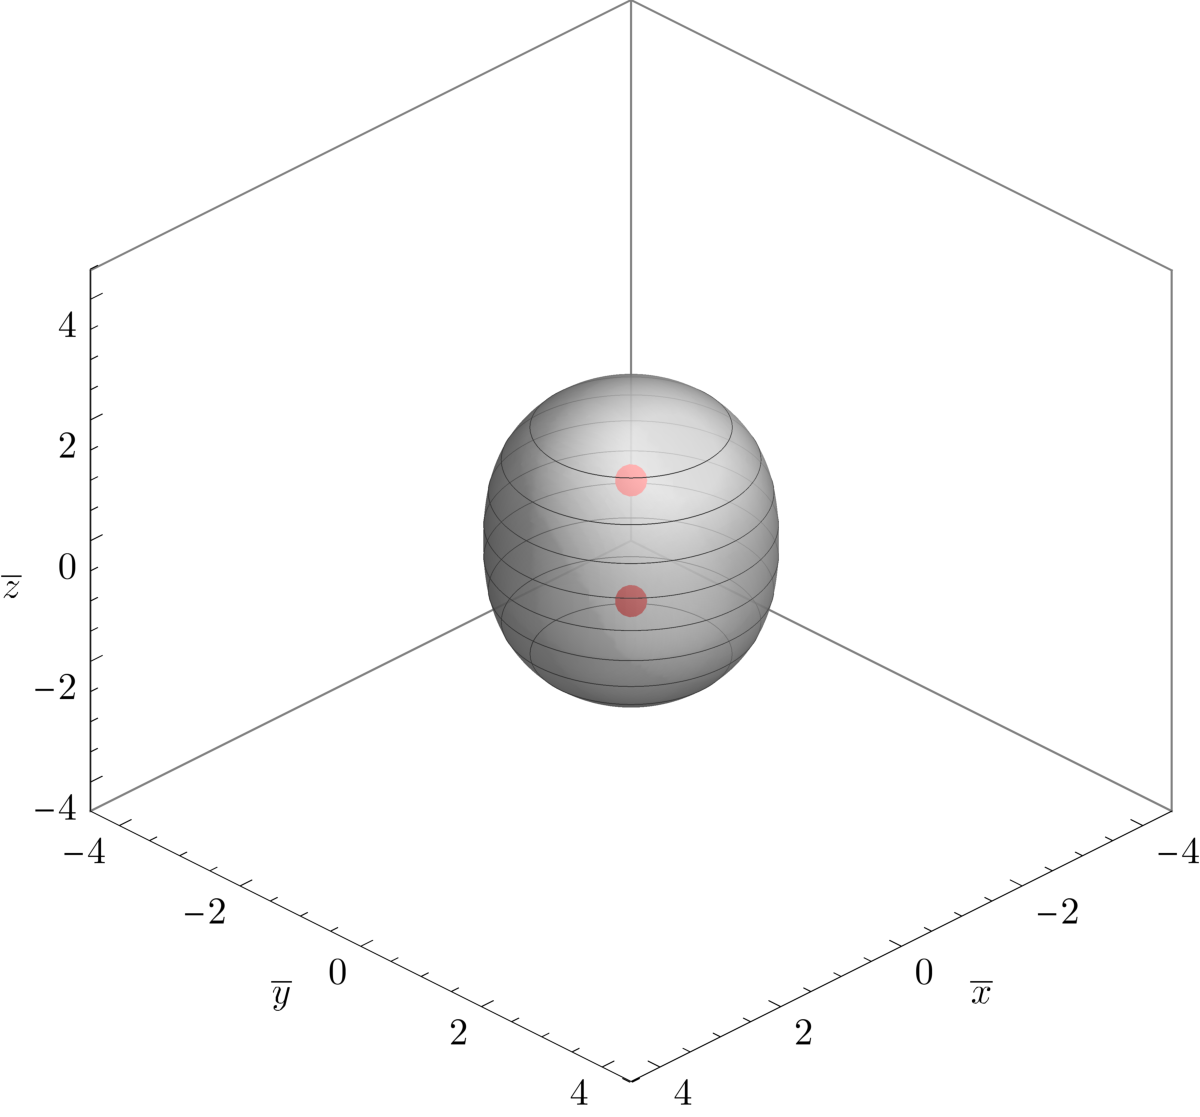
\includegraphics[width = 0.43\linewidth]{img/penrose_binaries/mp/ergo_1.pdf}
    \label{ch:penrose_binaries/fig:splitting_1}
  }
  \subfloat[$\mu=-0.6$]{
    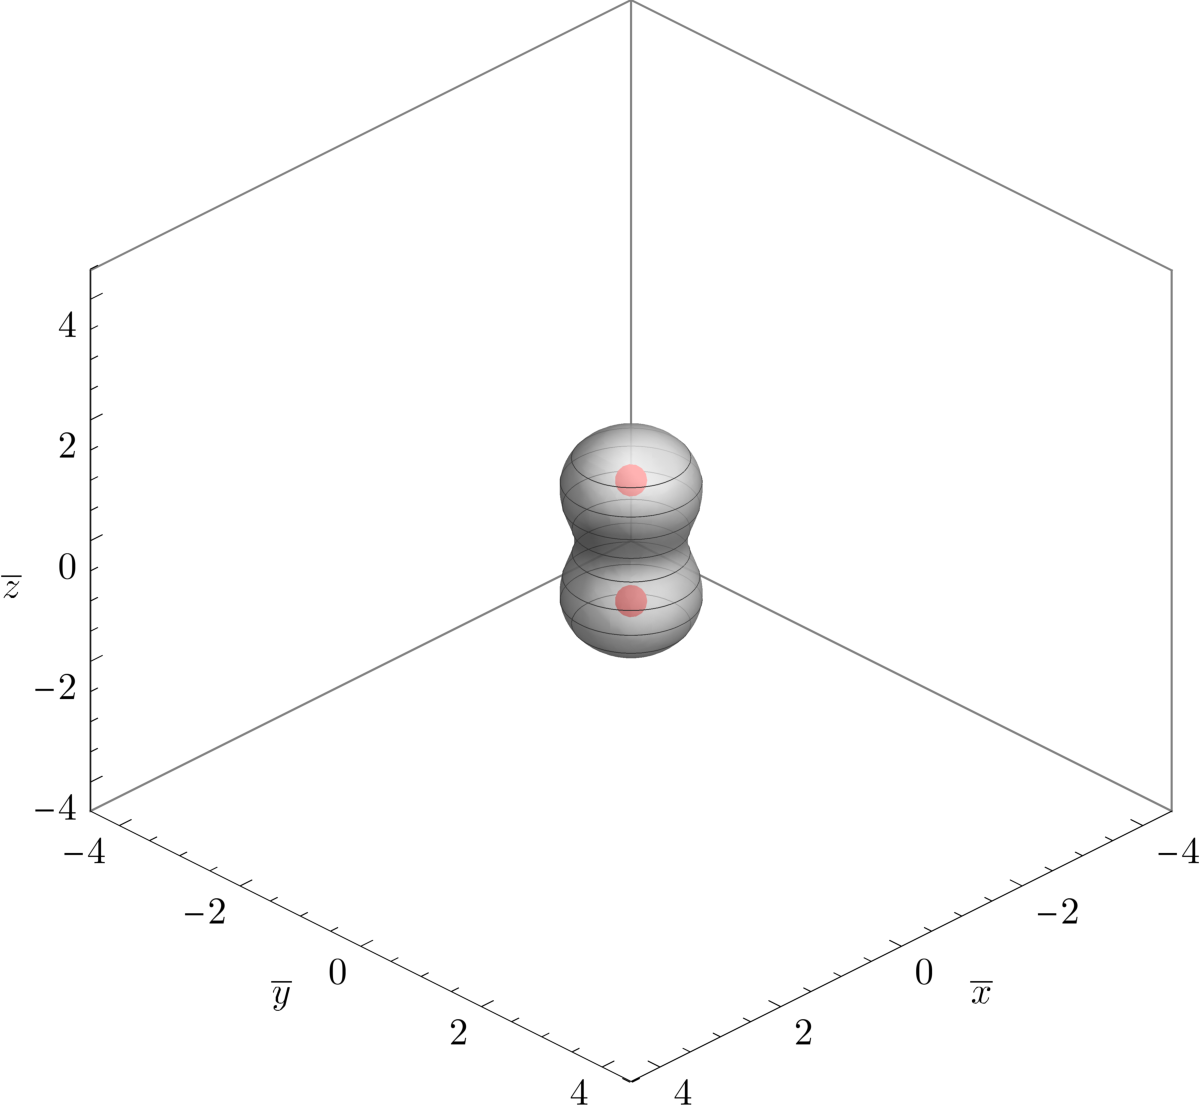
\includegraphics[width = 0.43\linewidth]{img/penrose_binaries/mp/ergo_2.pdf}
    \label{ch:penrose_binaries/fig:splitting_2}
  }
  \newline
  \subfloat[$\mu=-0.5$]{
    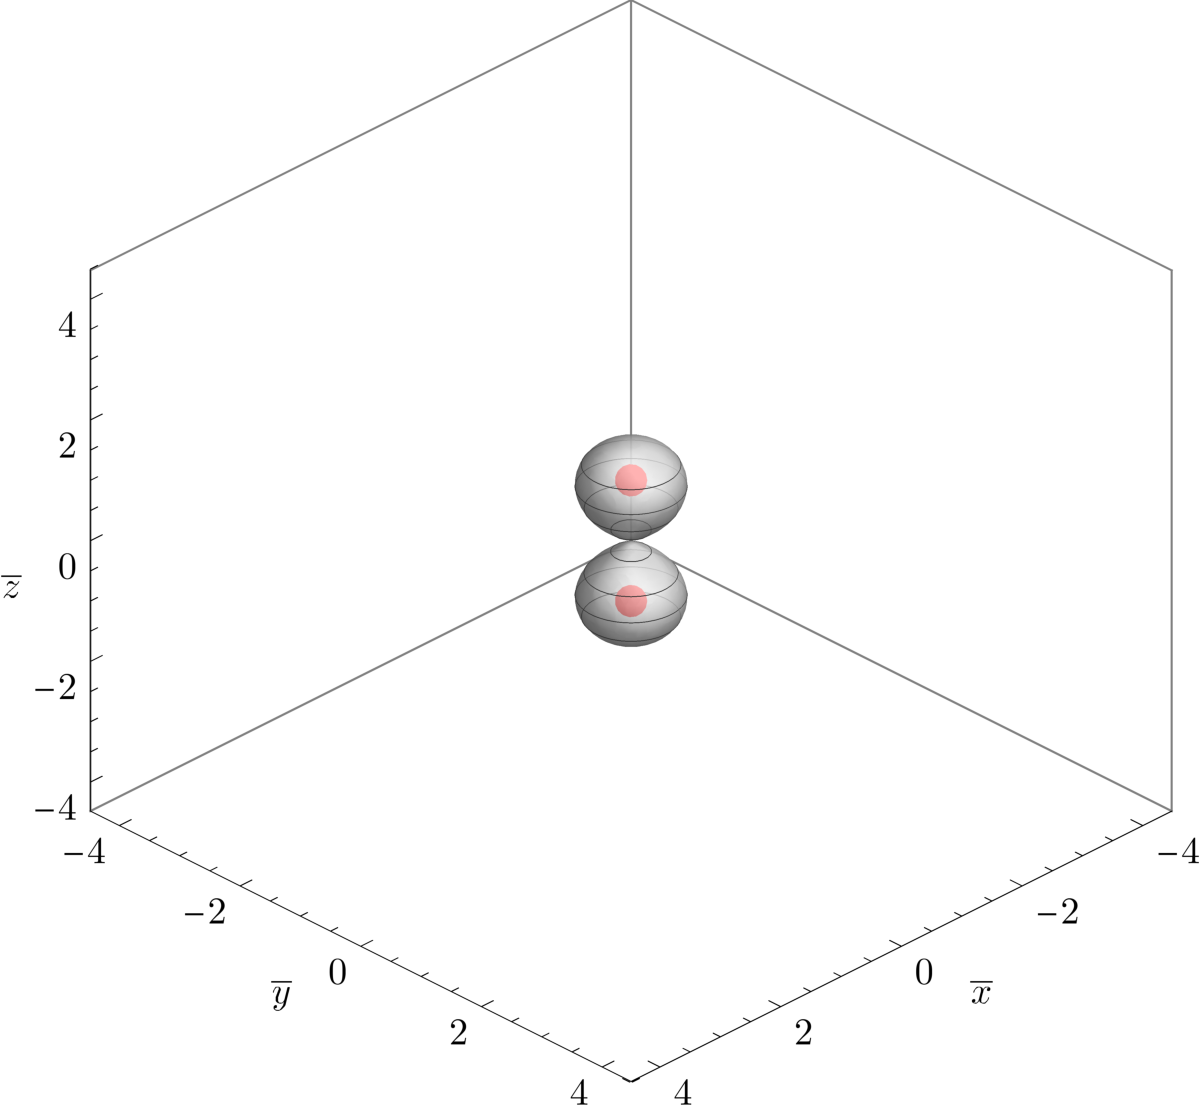
\includegraphics[width = 0.43\linewidth]{img/penrose_binaries/mp/ergo_3.pdf}
    \label{ch:penrose_binaries/fig:splitting_3}
  }
  \subfloat[$\mu=-0.35$]{
    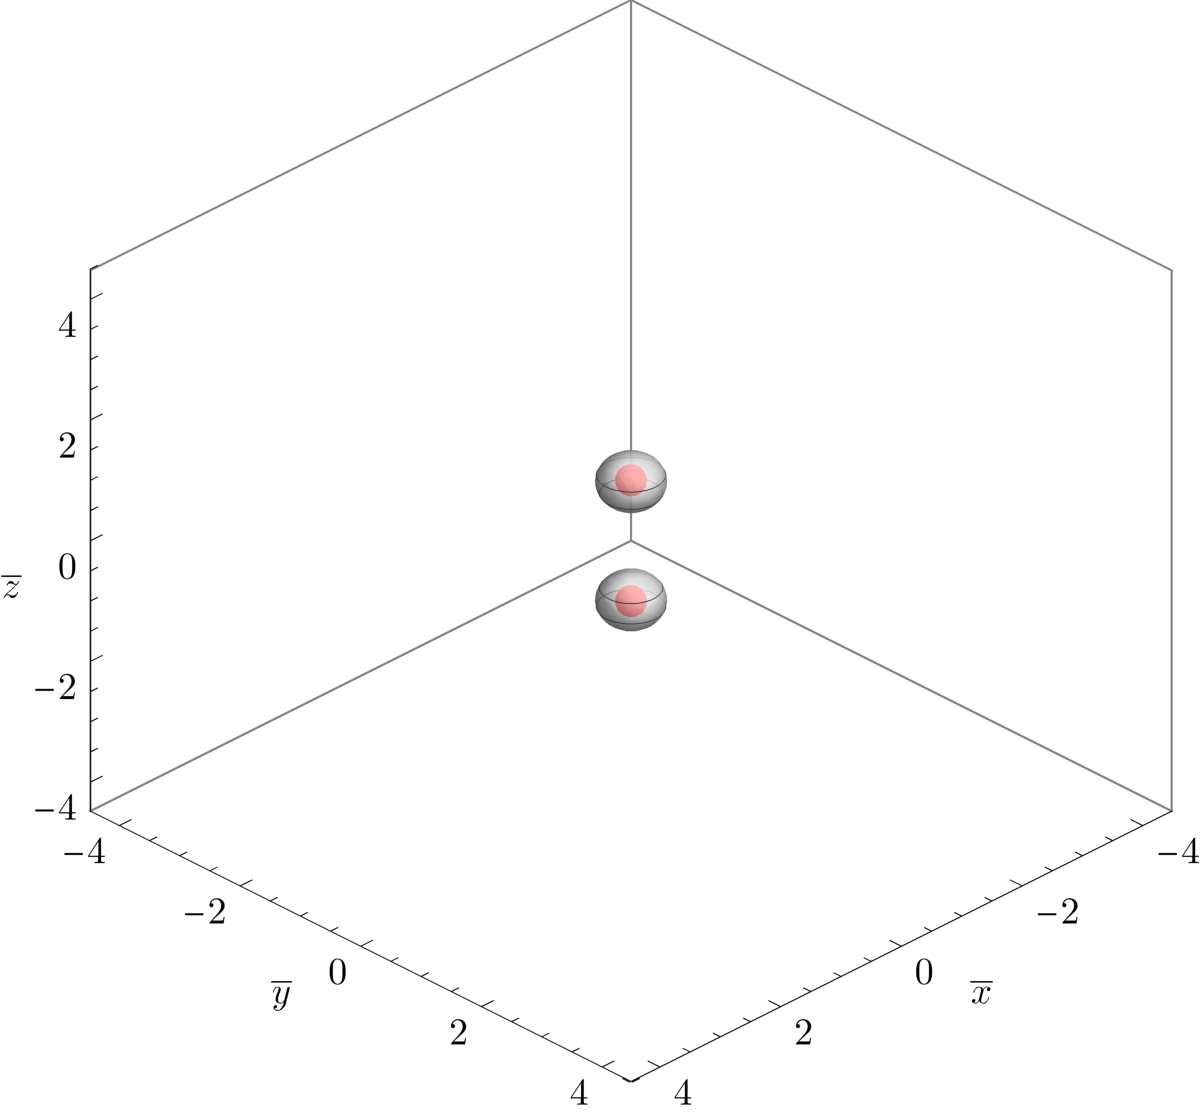
\includegraphics[width = 0.43\linewidth]{img/penrose_binaries/mp/ergo_4.pdf}
    \label{ch:penrose_binaries/fig:splitting_4}
  }
  \caption{Splitting and shrinking of the generalized ergosphere caused by an increase in the charge-to-mass ratio $\mu$ of a test particle. The separation parameter and mass-ratio are kept fixed at $\alpha = 1$ and $M = 1$, respectively. Note that the splitting produces two symmetric regions that are closer to the horizons.}
  \label{ch:penrose_binaries/fig:splitting_ergosphere_mass_increase}
\end{figure}

\begin{figure}[!htbp]
  \centering
  \subfloat[$M=2$]{
    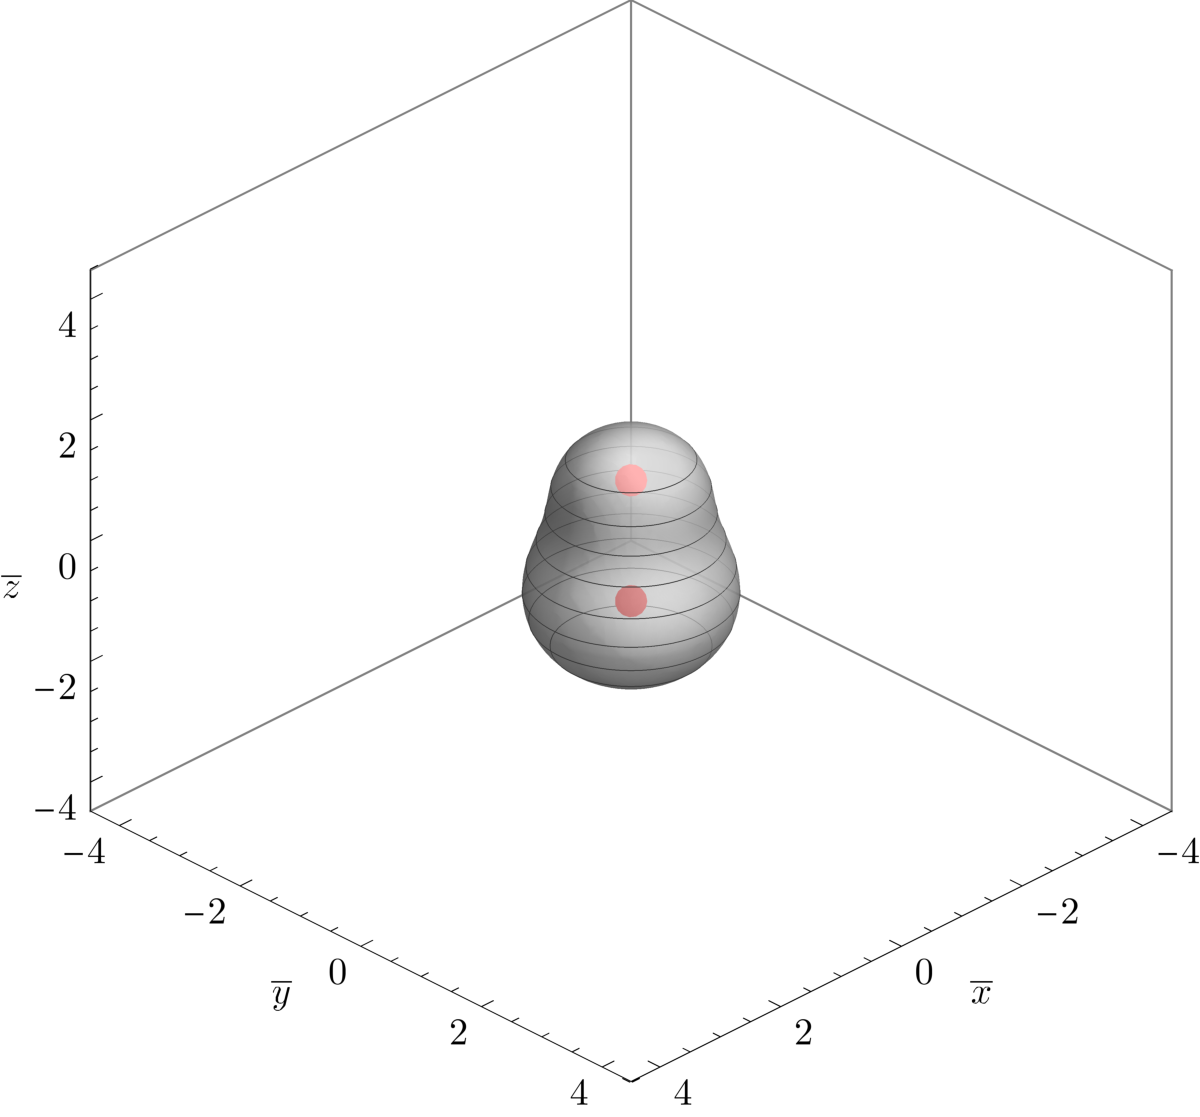
\includegraphics[width = 0.43\linewidth]{img/penrose_binaries/mp/ergo_5.pdf}
    \label{ch:penrose_binaries/fig:mass_increase_1}
  }
  \subfloat[$M=20/3$]{
    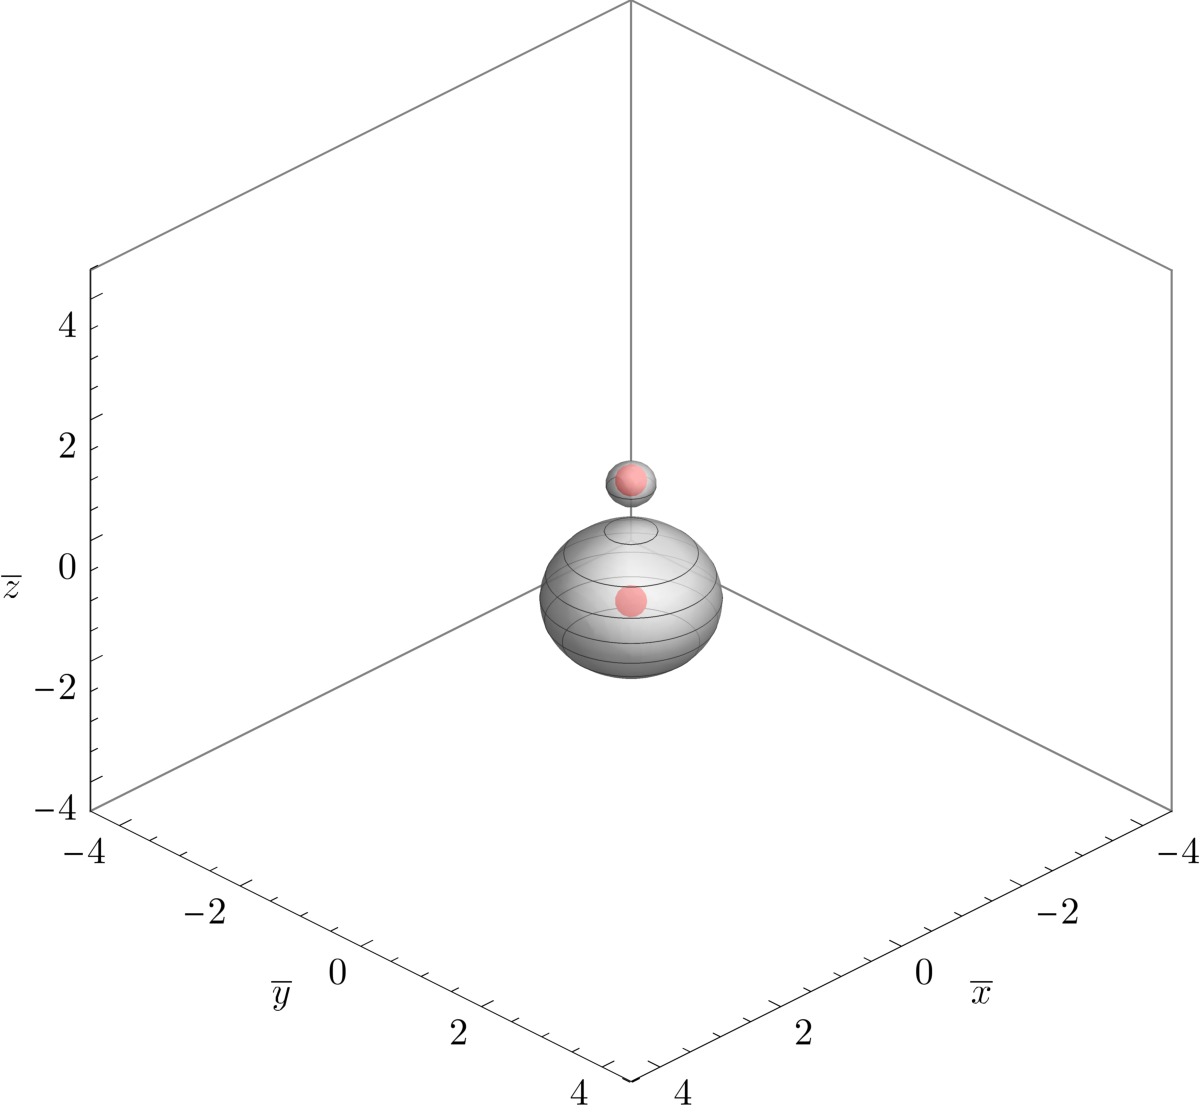
\includegraphics[width = 0.43\linewidth]{img/penrose_binaries/mp/ergo_6.pdf}
    \label{ch:penrose_binaries/fig:mass_increase_2}
  }
  \caption{Splitting of the generalized ergosphere caused by an increase in the mass ratio $M$. The separation parameter and charge-to-mass ratio are kept fixed at $\alpha = 1$ and $\mu = -1$, respectively. The final region is much larger around the heavier black hole.}
  \label{ch:penrose_binaries/fig:splitting_ergosphere_mass_increase}
\end{figure}

\begin{figure}[!htbp]
  \centering
  \subfloat[$\alpha=2$]{
    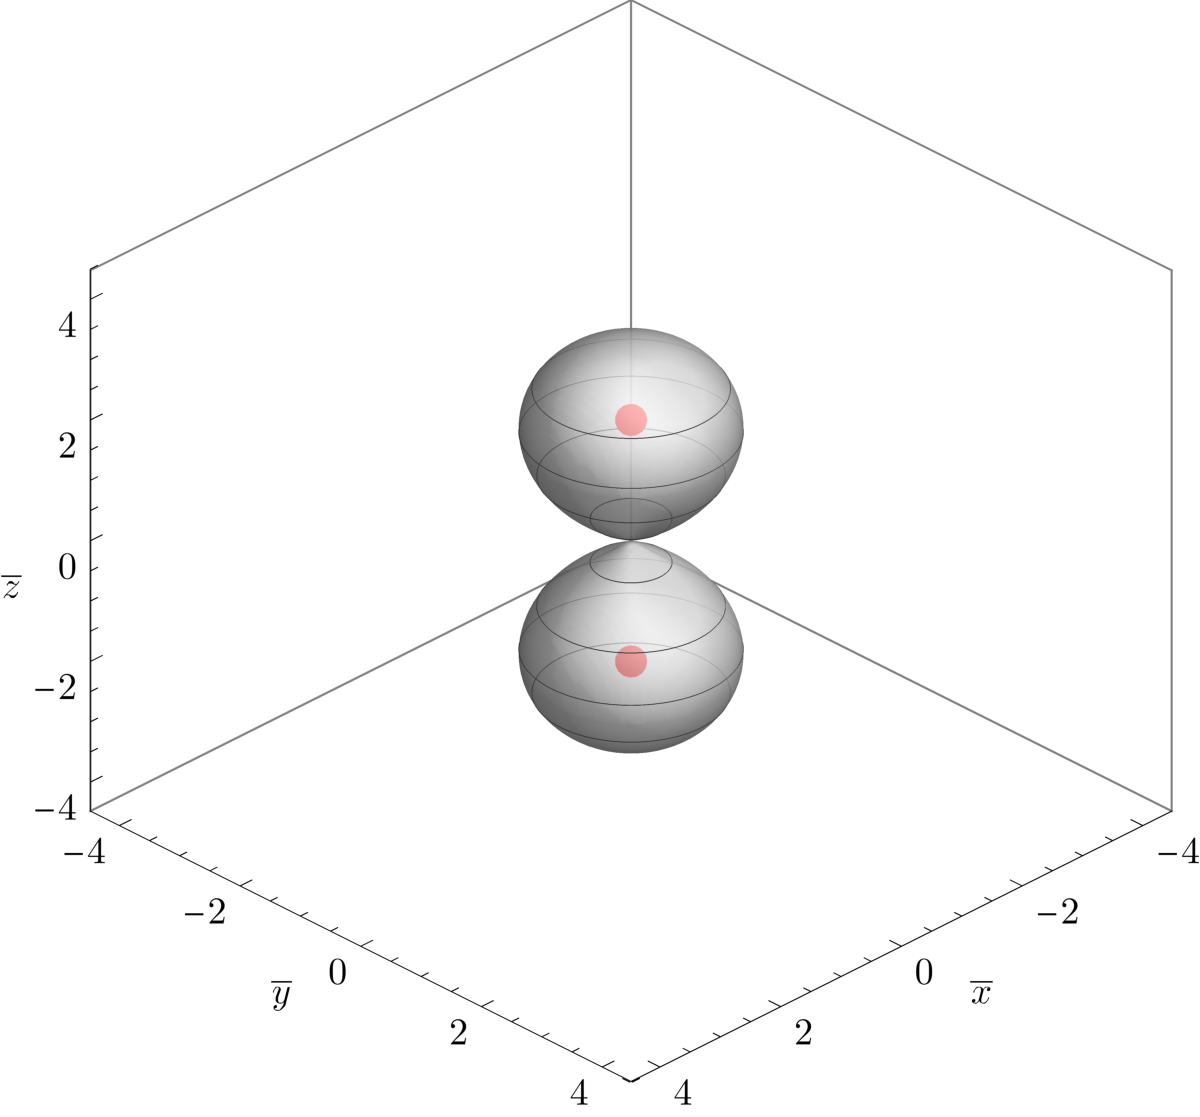
\includegraphics[width = 0.43\linewidth]{img/penrose_binaries/mp/ergo_7.pdf}
    \label{ch:penrose_binaries/fig:distance_1}
  }
  \subfloat[$\alpha=3$]{
    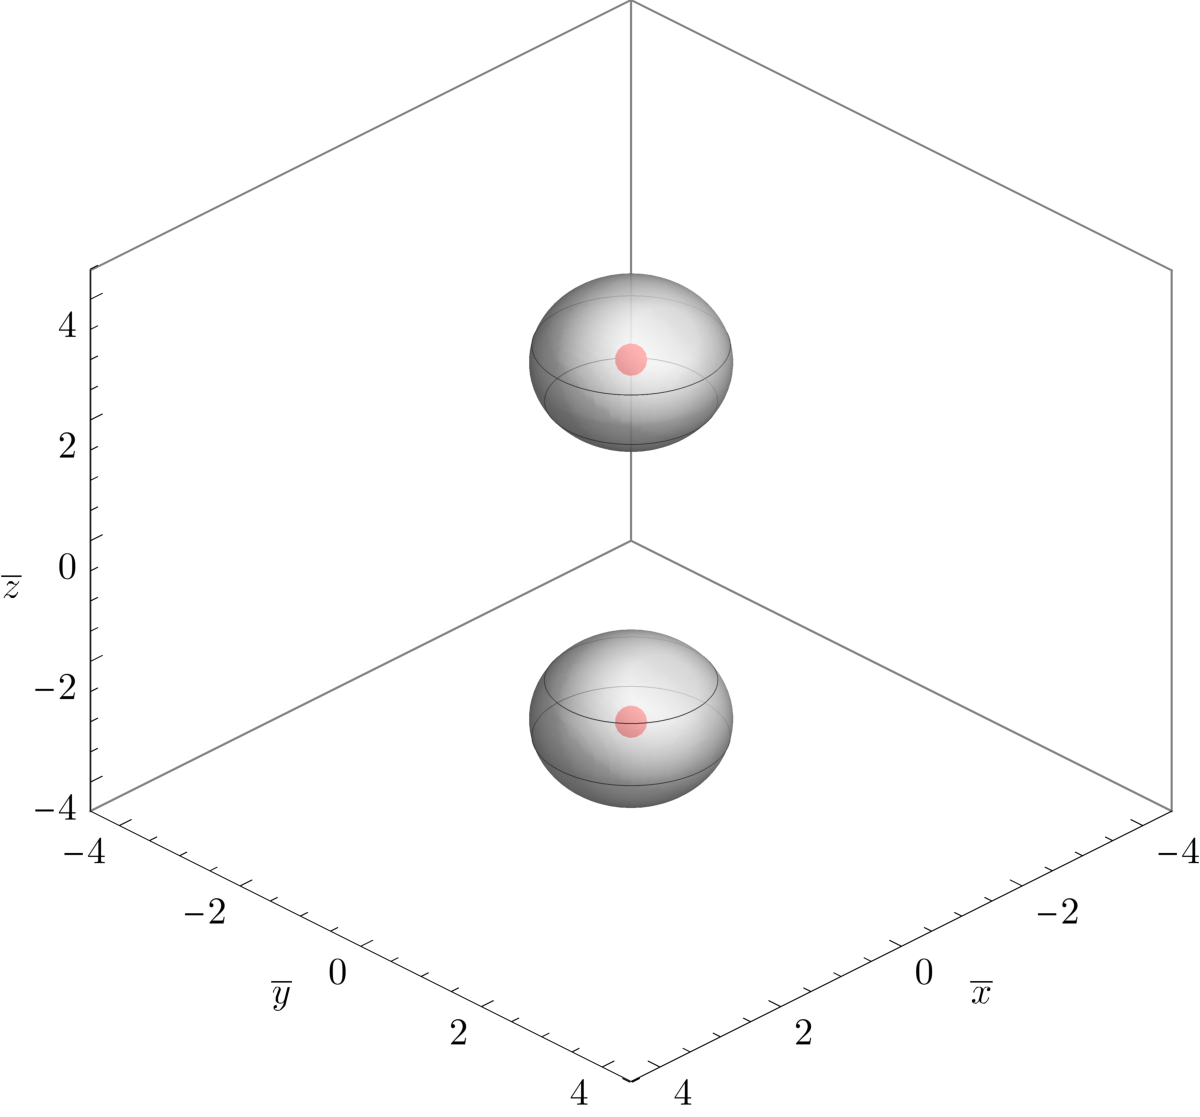
\includegraphics[width = 0.43\linewidth]{img/penrose_binaries/mp/ergo_8.pdf}
    \label{ch:penrose_binaries/fig:distance_2}
  }
  \caption{Splitting of the generalized ergosphere caused by an increase in the distance parameter $\alpha$ The mass ratio and charge-to-mass ratio are kept fixed at $M = 1$ and $\mu = -1$, respectively. The split region is symmetric and it is not closer farther than it previously was to either horizon.}
  \label{ch:penrose_binaries/fig:splitting_ergosphere_distance_increase}
\end{figure}

\subsection{Negative energy orbits and the Penrose process}

Having understood the notion of generalized ergospheres around binary black holes described by the MP metric, we are now in position to analyze the possibility of energy extraction in such spacetimes. The idea follows Penrose's original proposal~\cite{PENROSE1971} and its extension to RN black holes~\cite{RUFFINI1971,DENARDO1973}. The mechanism we shall explore consists in sending a negatively charged particle from sufficiently far away towards the binary black hole.  Once the particle enters the generalized ergosphere, we need it to break up into two pieces. Depending on how the splitting process is set up, one of the pieces will escape back to infinity with more energy than the incident particle had.

In order to accomplish this one needs three trajectories. The first one, with positive energy $E^{(0)} > 0$ and labeled $T^{(0)}$, must start outside the ergosphere and end inside it, at the point where the other two trajectories, labeled $T^{(1)}$ and $T^{(2)}$ start. One of them, let us say $T^{(1)}$, must have negative energy, i.e.~$E^{(1)}<0$, and, therefore, will remain confined inside the ergosphere. The other one, $T^{(2)}$, on the other hand, will have positive energy $E^{(2)} > E^{(0)}$, which allows it to escape the ergospohere and reach back infinity.

Suppose that the break-up of the particle occurs at $(\rho_0,\phi_0,z_0)$. Let $m^{(i)}$ and $\tens{P}{(i)}{\mu}$ denote, respectively, the mass and the the 4-momentum of the particle on trajectory $T^{(i)}$. The conservation of the four-momentum, applied at the break-up point, reads
\begin{equation}
  \tens{P}{(0)}{\mu} = \tens{P}{(1)}{\mu} + \tens{P}{(2)}{\mu}.
  \label{ch:penrose_binaries/eq:four_momentum_conservation}
\end{equation}
%
Each component of the vector equation above yields a different conservation equation with straightforward physical interpretation. The zero-component, for a start, is just the conservation of total energy, i.e.
\begin{equation}
  m^{(0)}E^{(0)} = m^{(1)}E^{(1)} + m^{(2)}E^{(2)},
  \label{ch:penrose_binaries/eq:conservation_of_charge_energy}
\end{equation}
while the angular component is simply the conservation of angular momentum around the $z$ axis, namely
\begin{equation}
  m^{(0)}L^{(0)} = m^{(1)}L^{(1)} + m^{(2)}L^{(2)}.
  \label{ch:penrose_binaries/eq:conservation_ang_mom}
\end{equation}
The other two components represent the conservation of linear momentum along the radial direction and along the $z$ axis, respectively
\begin{equation}
  \tens{m}{(0)}{}\tens{\dot{\rho}}{(0)}{} = \tens{m}{(1)}{}\tens{\dot{\rho}}{(1)}{} + \tens{m}{(2)}{}\tens{\dot{\rho}}{(2)}{}
  \label{ch:penrose_binaries/eq:conservation_rho}
\end{equation}
%
and
%
\begin{equation}
  \tens{m}{(0)}{}\tens{\dot{z}}{(0)}{} = \tens{m}{(1)}{}\tens{\dot{z}}{(1)}{} + \tens{m}{(2)}{}\tens{\dot{z}}{(2)}{},
  \label{ch:penrose_binaries/eq:conservation_z}
\end{equation}

where all the derivatives are to be evaluated at the break-up point $(\rho_0,\phi_0,z_0)$.

Because we've assumed that $E^{(1)} < 0$, it's easy to see from \eqref{ch:penrose_binaries/eq:conservation_of_charge_energy} that the particle on trajectory $T^{(2)}$ will be more energetic than the particle on trajectory $T^{(0)}$ and thus it has \emph{gained} energy during the split-up process. Obviously this extra energy must come from somewhere. In Penrose's original proposal, the extra energy came from a small loss of angular momentum in the background Kerr black hole. This idea can be readily extended to charged black holes: now instead of angular momentum, the black hole donates part of it's electromagnetic energy to an outgoing particle. One might naturally ask how much energy can be extracted using this process. This was not answered by Penrose but by Christodoulou in Ref.~\cite{CHRISTODOULOU1970}. It turns out that the mass of a black hole cannot be smaller than a certain \emph{irreducible mass}, and about 50\% of a charged black hole's electromagnetic energy and 29\% of a rotating black hole's angular momentum can be extracted through this process. An important variation of the Penrose process is to consider particle collisions, instead of break-ups. This is befittingly known as the collisional Penrose process and it is capable of producing much more energetic ejecta that could be a potential source of gamma rays and high energy cosmic rays (see e.g.~\cite{PhysRevLett.114.251103}), however, in our work we will only focus on the non-colisional version the Penrose process.

The existence of a generalized ergosphere as we've shown, indicates that negative energy orbits can exist and thus electromagnetic energy can be extracted from a MP binary through the Penrose process. However we are not only interested in where these orbits are located but also on some of their features, e.g., weather they fall into one of the black holes or keep orbiting the system in a closed orbit. In the following sections we will describe briefly the characteristics of negative energy orbits constrained to two planes of motion around the system. This analysis will come into play later when we construct two explicit examples of the penrose process in action. We start by introducing two quantities, the \emph{effective energy} $E_{\text{eff}}(\rho,z)$ and the \emph{effective potential} $V_{\text{eff}}(\rho,z)$, given by

\begin{equation}
  E_{\text{eff}}(\rho,z) \equiv E - \mu\left(1 - \frac{1}{U(\rho,z)}\right)
  \label{ch:penrose_binaries/eq:effective_energy_definition}
\end{equation}
%
and

\begin{equation}
  V_{\text{eff}}(\rho,z) \equiv \frac{L^2}{\rho^2 U(\rho,z)^4} + \frac{1}{U(\rho,z)^2}.
  \label{ch:penrose_binaries/eq:effective_potential_definition}
\end{equation}

With that, we can recast Eq.~\eqref{ch:penrose_binaries/eq:alternative_expression_for_energy} as

\begin{equation}
  \dot{\rho}^2 + \dot{z}^2 = E_{\text{eff}}(\rho,z)^2 - V_{\text{eff}}(\rho,z).
  \label{ch:penrose_binaries/eq:first_order_ode_for_orbits}
\end{equation}

\subsubsection{Orbits in the \texorpdfstring{$\rho$}{$\symit{rho}$}-$z$ plane}

One can easily see that by setting $L$ (and thus $\dot{\phi}$) to zero, the particle's orbit will be constrained to a plane that contains both of the black holes, which we call the $\rho$-$z$ plane. Because of the system's cylindrical symmetry one can set $\phi = 0$ without any loss of generality. To be able to integrate the equations of motion \eqref{ch:penrose_binaries/eq:ode_for_rho_motion} and \eqref{ch:penrose_binaries/eq:ode_for_z_motion} one must specify the remaining 4 initial conditions for $\rho$, $z$ and their time derivatives. Note however that $E$, $\dot{\rho}$ and $\dot{z}$ are related trough \eqref{ch:penrose_binaries/eq:first_order_ode_for_orbits} and thus it suffices to choose $\rho(0)$, $z(0)$, $\dot{z}(0)$ and $E$ while using \eqref{ch:penrose_binaries/eq:first_order_ode_for_orbits} to determine $\dot{\rho}(0)$.

In order to visualize the orbits we employ once again Cartesian-like coordinates $(\overline{x},\overline{y},\overline{z})$ reescaled by $M_1$, $M$ as the system's mass-ratio and $\alpha$ as it's separation parameter. In Figs.~\ref{ch:penrose_binaries/fig:orbit_1} and \ref{ch:penrose_binaries/fig:orbit_2} the event horizons are represented by black dots and the spacetime parameters were fixed at $M = \alpha = 1$. Additionally, because our process for finding $\dot{\rho}(0)$ involves square roots we use solid black lines for orbits resulting from the positive solution and dashed black lines for the negative solution. By extensively testing for many different initial conditions, we found that most orbits end up in either of the two black holes as in Fig.~\ref{ch:penrose_binaries/fig:orbit_1}. This is not surprising, as particles that follow negative energy orbits must always be charged oppositely to the black holes and thus they will always be electrically attracted towards the horizons. On the other hand, by choosing parameters very carefully, one is be able to find highly unstable but closed orbits as in Fig.~\ref{ch:penrose_binaries/fig:orbit_2}.

At a first glance, closed negative energy orbits might cause some concern as they never fall into one of the horizons and thus never effectively interact with the black holes to cause them to loose a small amount of electric charge but one must keep in mind that in the MP spacetime such orbits are always unstable and are completely within the generalized ergosphere. Additionally, the existence of closed negative energy orbits is not an exclusive feature of the MP metric. Usually these orbits occur only \emph{inside} event horizons or in naked singularities. Stuchlik has shown in Ref.~\cite{STUCHLIK1980} that there can exist stable circular orbits of negative energy around a Kerr naked singularity and that the Penrose process can effectively take place using said orbits. Patil and collaborators in Ref.~ \cite{PATIL2016} have even used this fact to construct a model to explain the origin of ultra high energy particles detected on Earth as a result of the colisional Penrose process in a slightly over spinning Kerr black hole. Similarly, Mukherjee and Nayak  in Ref.~\cite{MUKHERJEE2018} have used the colisional Penrose process in a Kerr naked singularity with orbits outside the equatorial plane to construct a model for energetic outgoing particle jets. In some situations though, closed negative energy orbits can exist outside of the event horizon as Prasana and Dadhich have shown in Ref.~\cite{PRASANA1982} in the spacetime of a Kerr black hole immersed in an external magnetic field that is regular up to the event horizon. More recently Felice and collaborators in Ref.~\cite{FELICE2004} also have shown that magnetized particles in a Kerr black hole can give rise to stable circular orbits of negative energy inside the ergosphere. Therefore, these unstable orbits that we've found are not violating any underlying fundamental principle.

\begin{figure}[!htbp]
  \centering
  \subfloat[$\overline{\rho}(0) = 0$, $\overline{z}(0) = 4$, $\dot{\overline{z}} = 0$, $E = -0.1$, $\mu = -4$]{
    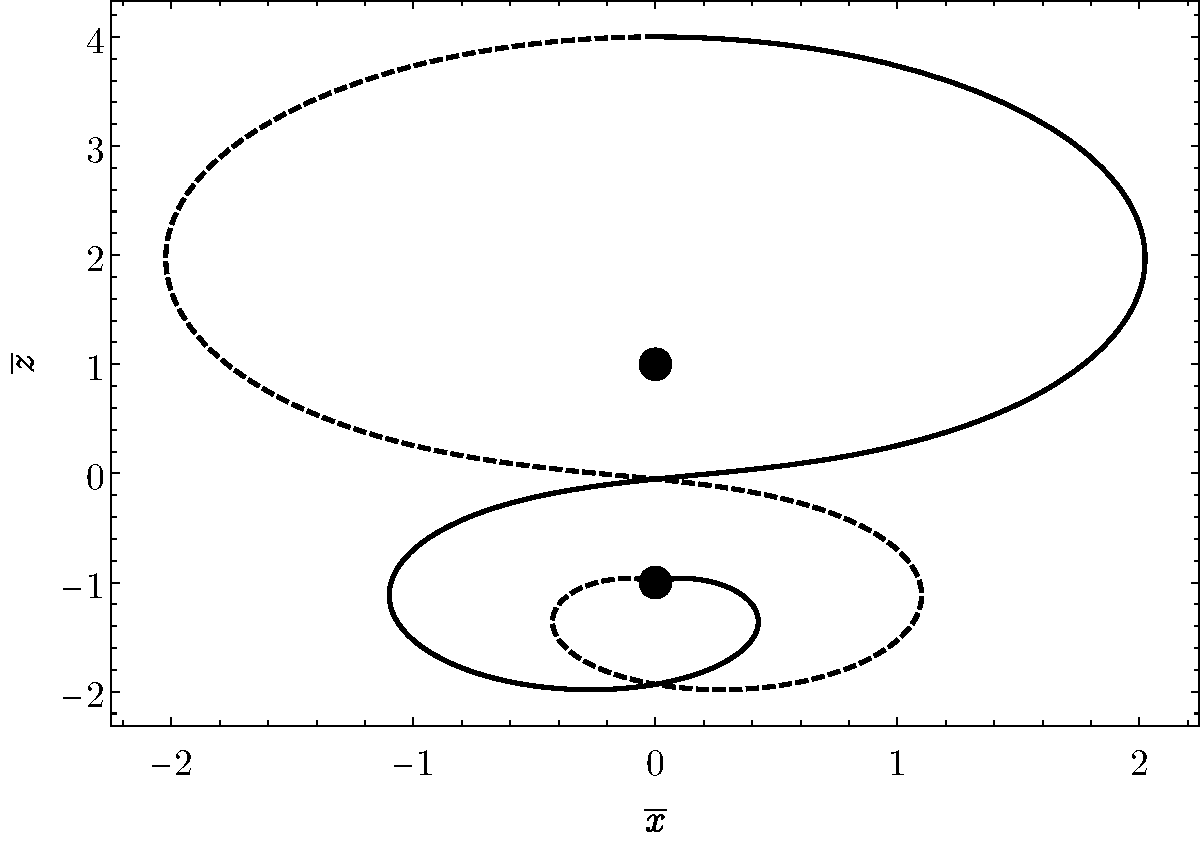
\includegraphics[width = 0.51\linewidth]{img/penrose_binaries/mp/orbit_1.pdf}
    \label{ch:penrose_binaries/fig:orbit_1}
  }
  \subfloat[$\overline{\rho}(0) = 0$, $\overline{z}(0) = 4.06$, $\dot{\overline{z}} = 0$, $E = -1$, $\mu = -9.63222$]{
    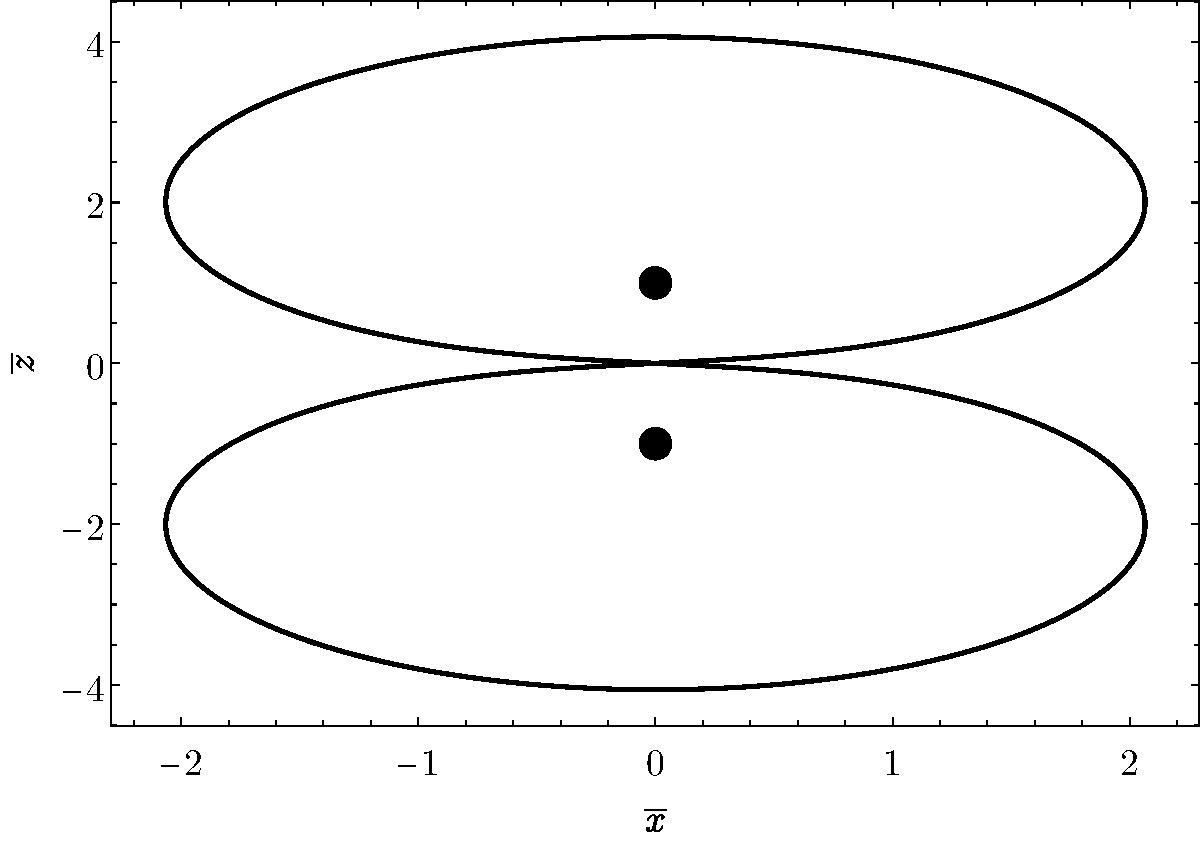
\includegraphics[width = 0.51\linewidth]{img/penrose_binaries/mp/orbit_2.pdf}
    \label{ch:penrose_binaries/fig:orbit_2}
  }
  \caption{Two different types of orbits in the $\rho$-$z$ plane: terminating (left) and closed (right). Initial conditions used for each orbits are presented in their respective captions. The dashed trajectory represents that of negative $\dot{\overline{\rho}}(0)$.}
  \label{ch:penrose_binaries/fig:rho_z_orbits}
\end{figure}

\subsubsection{Orbits in the $z=0$ plane}

If we set $z(0) = \dot{z}(0) = 0$ we confine the particle's motion to the plane exactly in between the two black holes and once the background spacetime parameters have been set the trajectory can now be readily determined using only Eq.~\eqref{ch:penrose_binaries/eq:first_order_ode_for_orbits} with appropriate values for $\rho(0)$, $\phi(0)$, $L$, $E$ and $\mu$. Thanks to the constrained motion we can now take full advantage of the effective potential formulation that we've introduced earlier. Our search revealed that particles with negative energy in this plane stay in a perpetual oscillatory motion either in straight lines or more complicated precessing orbits, depending on the value of $L$. These oscilating orbits are similar in nature to the closed orbits found in the $\rho$-$z$ plane as they also don't fall towards either of the black holes but they are stable in the sense that they do not require any fine tuning of the orbital parameters to be found, although they are globally unstable as any perturbation along the $z$ direction will cause the to fall towards one of the black holes. Proceeding with the same rescaling by $M_1$ scheme we've adopted so far, we plot in Figs.~\ref{ch:penrose_binaries/fig:orbit_z_1} and \ref{ch:penrose_binaries/fig:orbit_z_2} two oscillating orbits for a binary system with $M = \alpha = 1$. Note that if an infinite amount of time s allowed to pass, a particle following these trajectories will have swept the whole finite area between the minimum and maximum values attained by $\overline{\rho}$ during motion.

It's very hard (or even impossible) to obtain the orbital turning points of any oscilating orbit analytically by solving $E_{\text{eff}}(\rho,0)^2 - V_{\text{eff}}(\rho,0) = 0$ for $\rho$ as one can show that the problem reduces to finding the roots of a sixth-order polynomial equation. Despite that, its quite easy to find the roots of the polynomial numerically after the orbital parameters have been chosen and thus this is the approach we've adopted as a complete and rigorous analysis of the orbital turning points go beyond the scope of this work. In Figs.~\ref{ch:penrose_binaries/fig:veff_for_3} and \ref{ch:penrose_binaries/fig:veff_for_4} we plot the squared effective energy and the effective potential to the orbits described by \ref{ch:penrose_binaries/fig:orbit_z_1} and \ref{ch:penrose_binaries/fig:orbit_z_2} respectively and give their turning points. The effective potential is represented by a solid black line while the squared effective energy is represented by a dashed red line.

\begin{figure}[!htbp]
  \centering
  \subfloat[$\overline{\rho}(0) = 2$, $\phi(0) = 0$, $L = 2$, $E = -1$ and $\mu = -4$.]{
    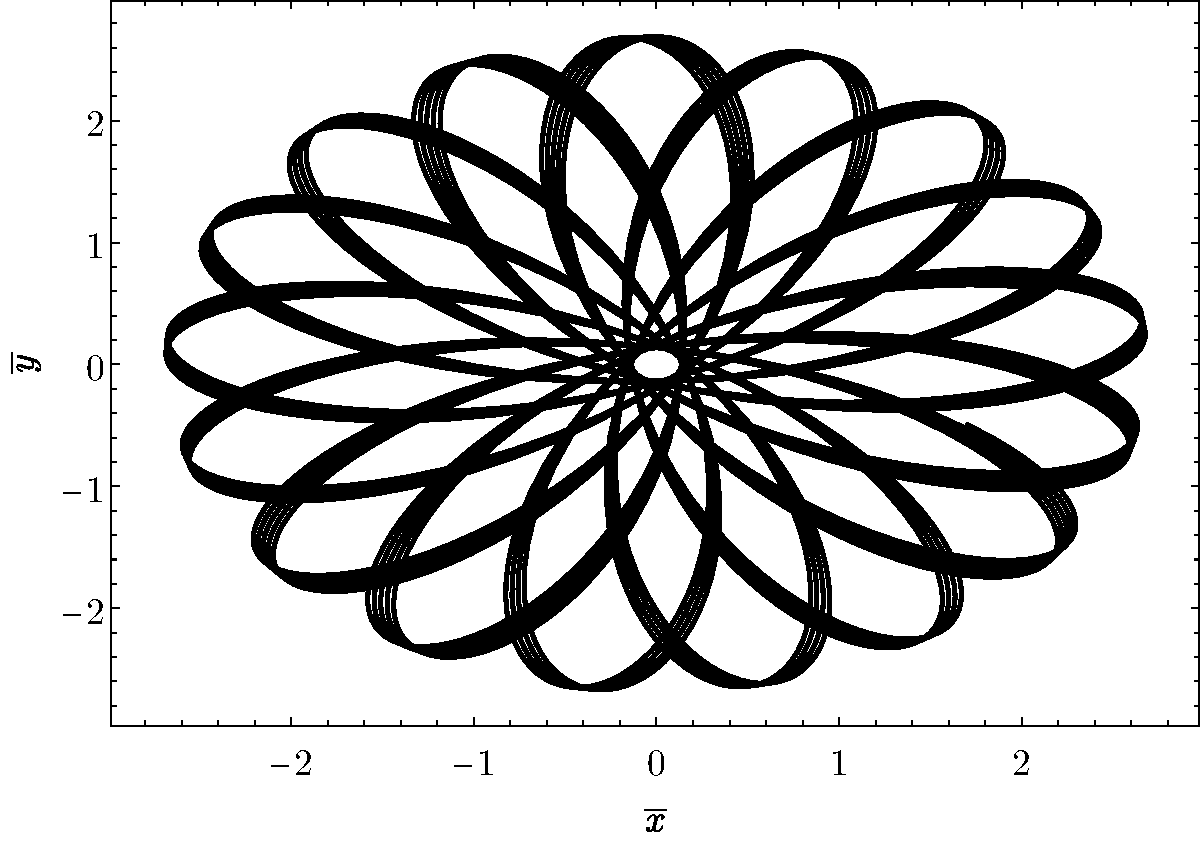
\includegraphics[width = 0.5\linewidth]{img/penrose_binaries/mp/orbit_3.pdf}
    \label{ch:penrose_binaries/fig:orbit_z_1}
  }
  \subfloat[$\overline{\rho}(0) = 2$, $\phi(0) = 0$, $L = 10$, $E = -1$ and $\mu = -6$.]{
    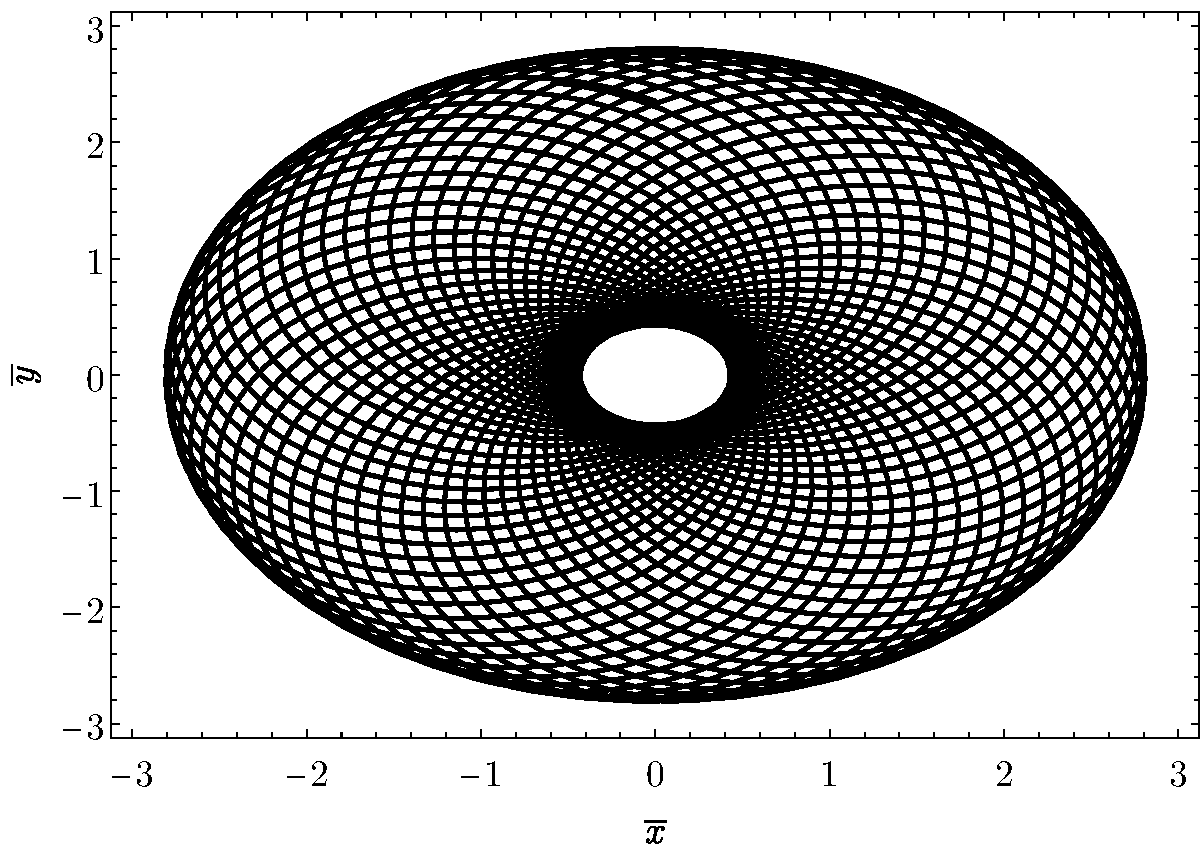
\includegraphics[width = 0.5\linewidth]{img/penrose_binaries/mp/orbit_4.pdf}
    \label{ch:penrose_binaries/fig:orbit_z_2}
  }
  \caption{Two oscilating orbits in the $z = 0$ symmetry plane. Note that the area swept by a particle in either orbit after an infinite amount of time is finite and proportional to the difference between the and outer orbital radii.}
  \label{ch:penrose_binaries/fig:z_orbits}
\end{figure}

\begin{figure}[!htbp]
  \centering
  \subfloat[Turning points: $\overline{\rho}_{\text{min}} = 0.1386$ and $\overline{\rho}_{\text{max}} = 2.6883$.]{
  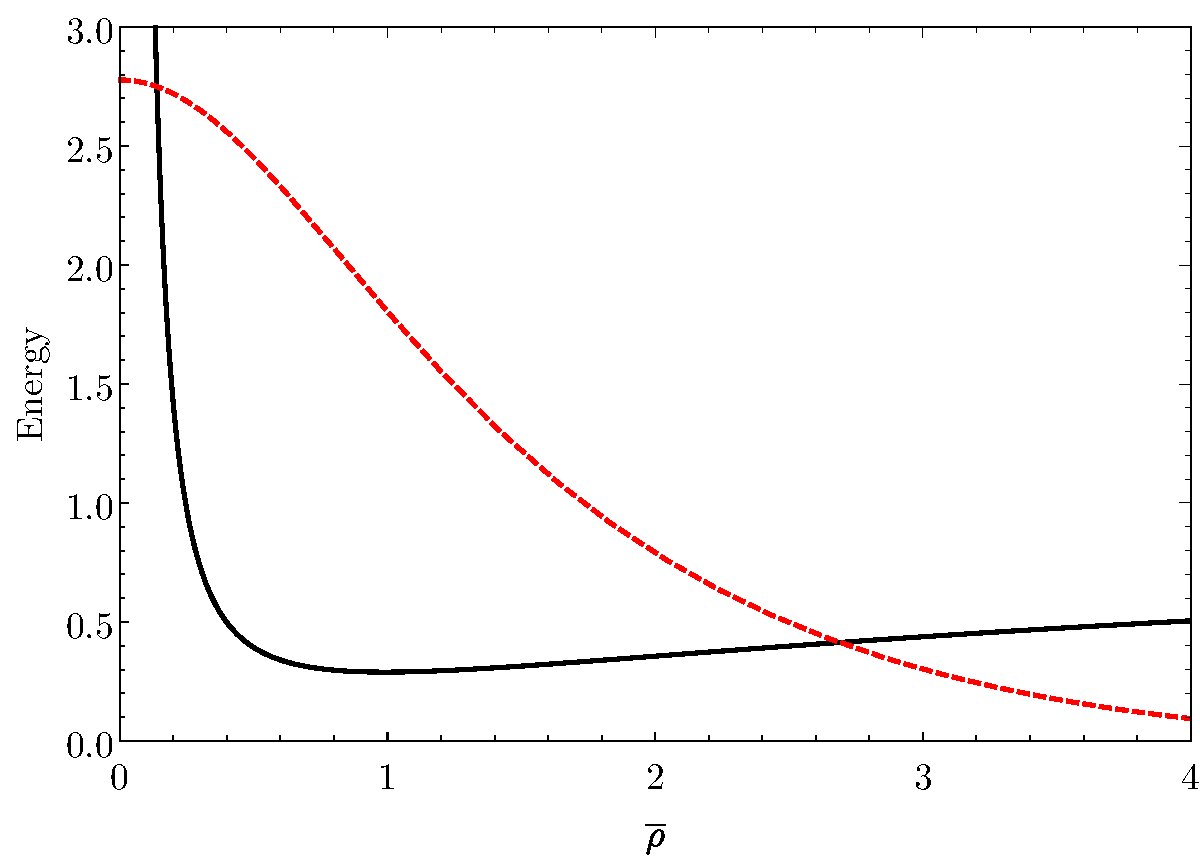
\includegraphics[width = 0.5\linewidth]{img/penrose_binaries/mp/veff_for_3.pdf}
  \label{ch:penrose_binaries/fig:veff_for_3}
  }
  \subfloat[Turning points: $\overline{\rho}_{\text{min}} = 0.4352$ and $\overline{\rho}_{\text{max}} = 2.8091$.]{
  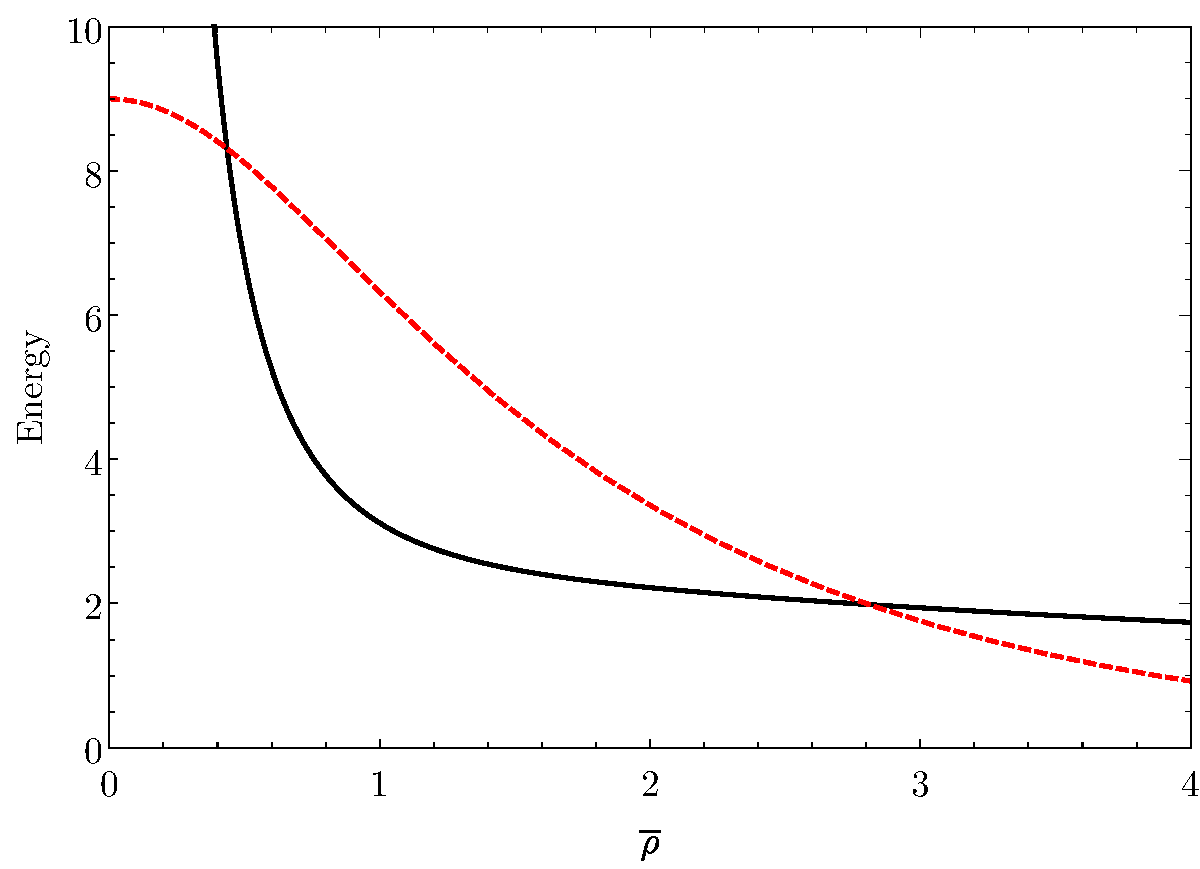
\includegraphics[width = 0.5\linewidth]{img/penrose_binaries/mp/veff_for_4.pdf}
  \label{ch:penrose_binaries/fig:veff_for_4}
  }
  \caption{The effective potential (solid black line) and squared effective energy (dashed red line) for the orbits depicted in \ref{ch:penrose_binaries/fig:orbit_z_1} (left) and \ref{ch:penrose_binaries/fig:orbit_z_2} (right).}
  \label{ch:penrose_binaries/fig:veff_graphs}
\end{figure}

\subsection{Examples of Penrose processes}

Let us now give concrete examples of energy extraction in a binary black hole spacetime. As we've already seen, under a few different circumstances such as when the black holes are sufficiently apart, the charge-to-mass ratios of the fragments are sufficiently small or when the mass ratio is large, the ergosphere is composed by two disconnected regions. When this happens, the only way to extract energy from the binary is by having the negative energy trajectory reaching the event horizon of one of the black holes. Consequently, the negative energy particle will eventually reach one of the singularities. If, on the other hand, the black holes are sufficiently close to each other, an interesting possibility opens up. Instead of having the negative energy orbit reach one of the event horizons, we can engineer the break up so that it will exist forever outside the black holes, confined to the ergosphere of the binary using trajectories like those in Figs.~\ref{ch:penrose_binaries/fig:orbit_2}, \ref{ch:penrose_binaries/fig:orbit_z_1} or \ref{ch:penrose_binaries/fig:orbit_z_2}. Naturally, $T^{(1)}$ (the negative energy trajectory) will only make sense physically if $\dot{\rho}^2 \ge 0$ everywhere. Thus, once $E^{(1)}$ and $L^{(1)}$ have been specified, the requirement that\label{ch:penrose_binaries/eq:effective_potential_orbit_equation} be non-negative constrains the possible value for the break-up coordinate $\rho_0$. Note that the angular break-up coordinate $\phi_0$ is irrelevant due to the system being symmetric with respect to rotations around the $z$ axis.

To construct an example, we start of by selecting a negative energy trajectory $T^{(1)}$ and a break-up point inside the ergosphere. After that, we construct an arbitrary orbit of positive energy that reaches infinity to serve as $T^{(2)}$. By solving the system formed by Eqs.~\eqref{ch:penrose_binaries/eq:four_momentum_conservation}-\eqref{ch:penrose_binaries/eq:conservation_rho} together with the conservation of electric charge, one is able to determine all of the orbital parameters for $T^{(0)}$. In Table~\ref{ch:penrose_binaries/tab:exemple_orbital_parameters_1} we summarize the orbital parameters for the process depicted in Fig. \ref{ch:penrose_binaries/fig:penrose_example_1}. The particle comes in orbit $T^{(1)}$ represented by the solid black curve and then splits at the grey dot into a negative energy orbit $T^{(1)}$ represented by a blue dotted curve and a positive energy orbit $T^{(2)}$ represented by a red dashed curve. In this example, we've set the spacetime parameters at $M = \alpha = 1$ and the two black dots represent the black hole's event horizons. Note that the entire process is confined to the $\rho$-$z$ plane.

\begin{table}[!htbp]
  \centering
  \caption{Orbital parameters for an example Penrose process in the $\rho$-$z$ plane.}
  \begin{tabular}{c|c|c|c|c|c|c|c|}
    \cline{1-8}
    \multicolumn{1}{|c|}{$T^{(i)}$} & $\mu^{(i)}$ & $E^{(i)}$ & $L^{(i)}$ & $\rho_0^{(i)}$ & $z_0^{(i)}$ & $\dot{\rho}_0^{(i)}$ & $\dot{z}_0^{(i)}$ \\ \hline
    \multicolumn{1}{|c|}{$T^{(0)}$} & $0.16076$   & $3.93401$ & $0$       & $0$            & $4.06$      & $3.82283$            & $0$               \\ \hline
    \multicolumn{1}{|c|}{$T^{(1)}$} & $-9.63222$  & $-1$      & $0$       & $0$            & $4.06$      & $-2.21869$           & $0$               \\ \hline
    \multicolumn{1}{|c|}{$T^{(2)}$} & $10$        & $10$      & $0$       & $0$            & $4.06$      & $6.52697$            & $0$               \\ \hline
  \end{tabular}
  \label{ch:penrose_binaries/tab:exemple_orbital_parameters_1}
\end{table}

\begin{figure}[!htbp]
  \centering
  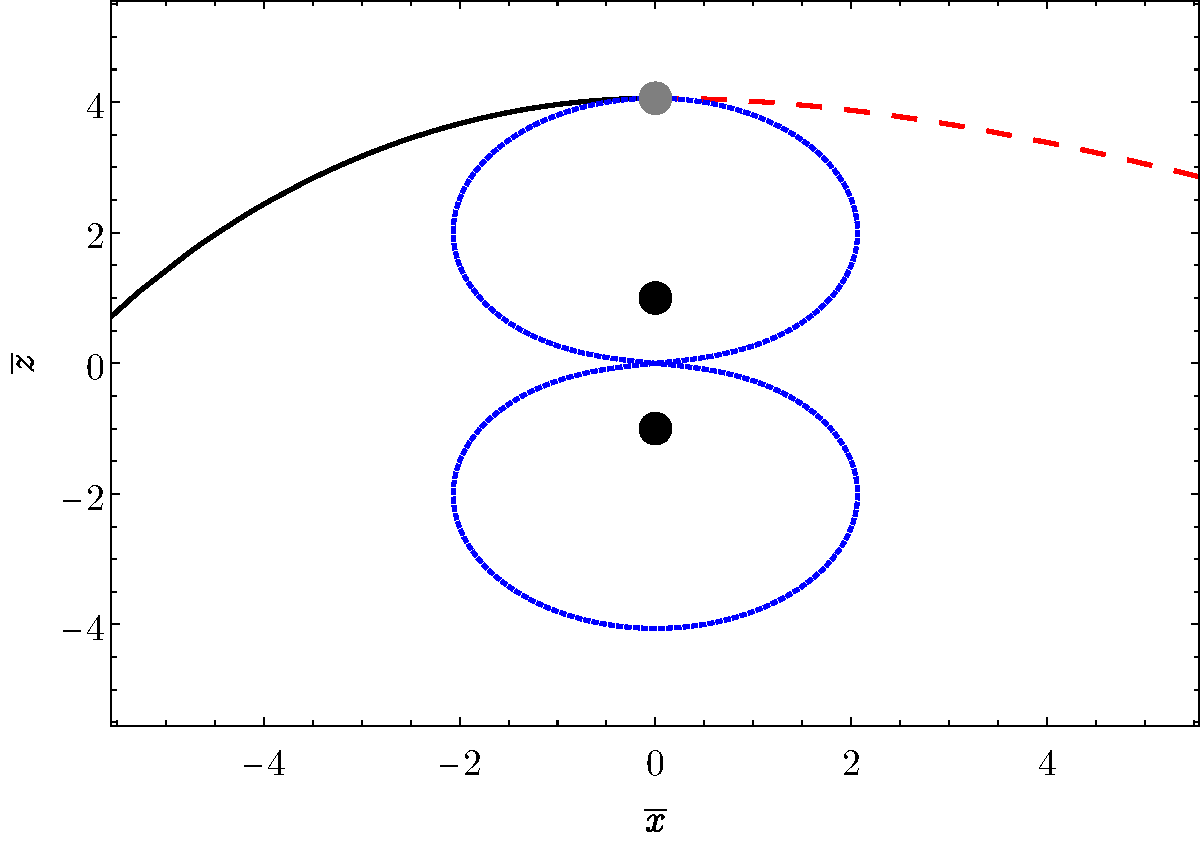
\includegraphics[scale = 0.4]{img/penrose_binaries/mp/penrose_xz.pdf}
  \caption{Example of a penrose process in the $\rho$-$z$ plane. The incoming trajectory (solid black) splits at the grey point into an negative energy (dotted blue) and increased energy (dashed red) orbit.}
  \label{ch:penrose_binaries/fig:penrose_example_1}
\end{figure}

If instead we choose to confine our orbits to the $z=0$ plane, by employing the same algorithm with the same background spacetime parameters as before, we obtain the orbital parameters described in Tab.~\ref{ch:penrose_binaries/tab:exemple_orbital_parameters_2} and depicted in Fig. \ref{ch:penrose_binaries/fig:penrose_example_2}. Here we've chosen to draw only a few periods of the oscilating trajectory $T^{(1)}$ to improve the figure's clarity.

\begin{table}[!htbp]
  \centering
  \caption{Orbital parameters for an example Penrose proces in the $z=0$ plane.}
  \begin{tabular}{c|c|c|c|c|c|c|c|}
    \cline{1-8}
    \multicolumn{1}{|c|}{$T^{(i)}$} & $\mu^{(i)}$ & $E^{(i)}$ & $L^{(i)}$ & $\rho_0^{(i)}$ & $z_0^{(i)}$ & $\dot{\rho}_0^{(i)}$ & $\dot{z}_0^{(i)}$ \\ \hline
    \multicolumn{1}{|c|}{$T^{(0)}$} & $-0.85050$  & $2.18701$ & $1.70101$ & $2$            & $0$         & $2.52301$            & $0$               \\ \hline
    \multicolumn{1}{|c|}{$T^{(1)}$} & $-4$        & $-1$      & $2$       & $2$            & $0$         & $-0.65820$           & $0$               \\ \hline
    \multicolumn{1}{|c|}{$T^{(2)}$} & $0.5$       & $10$      & $4$       & $2$            & $0$         & $-9.72474$           & $0$               \\ \hline
  \end{tabular}
  \label{ch:penrose_binaries/tab:exemple_orbital_parameters_2}
\end{table}

\begin{figure}[!htbp]
  \centering
  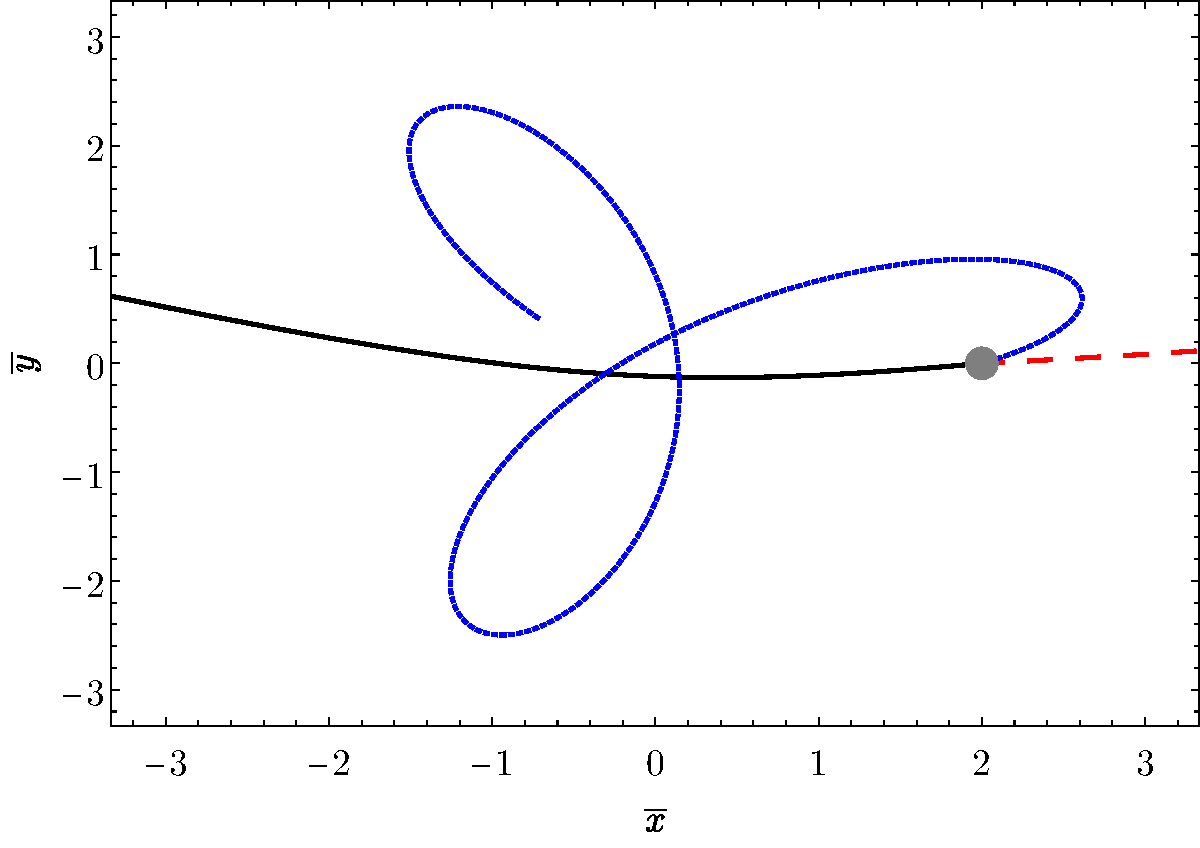
\includegraphics[scale = 0.43]{img/penrose_binaries/mp/penrose_xy.pdf}
  \caption{Example of a Penrose process that happens entirely on the $z=0$ plane of a MP binary black hole. Once again, the incoming trajectory (solid black) splits at the grey point into an negative energy (dotted blue) and increased energy (dashed red) orbit.}
  \label{ch:penrose_binaries/fig:penrose_example_2}
\end{figure}

\subsection{Efficiency of energy extraction}

The efficiency $\eta$ of the Penrose process can be trivially defined as the ratio between the energy input and output. Using Eq.~\eqref{ch:penrose_binaries/eq:conservation_of_charge_energy}, we can see that

\begin{equation}
  \eta = - \frac{m^{(1)}}{m^{(0)}} \frac{E^{(1)}}{E^{(0)}}.
  \label{ch:penrose_binaries/eq:penrose_efficiency_general}
\end{equation}

One can choose $E^{(1)} = 1$ and $m^{(1)}/m^{(0)} = 1$ without any loss of generality. Furthermore it's clear that in order to obtain maximum efficiency, one must choose $E^{(1)}$ to be as negative as possible, and thus of the form of Eq.~\eqref{ch:penrose_binaries/eq:minimum_energy}. With these choices, the efficiency becomes

\begin{equation}
  \eta = \mu^{(1)}\left(\frac{1}{U} - 1\right) - \frac{1}{U}.
  \label{ch:penrose_binaries/eq:penrose_efficiency_max}
\end{equation}

Notice that because \eqref{ch:penrose_binaries/eq:penrose_efficiency_max} depends on $U$, the efficiency depends on the particle's position. Using spherical coordinates centered around the origin, one can see that as $a\rightarrow 0$,

\begin{equation}
  \eta = -\frac{\mu^{(1)}(M_1 + M_2) + r}{M_1 + M_2 + r},
  \label{ch:penrose_binaries/eq:a_zero_efficiency}
\end{equation}
%
which is precisely the efficiency one would obtain for and extremal RN black hole of mass $M_1 + M_2$ in a coordinate system where the event horizon is a point. If the particle is locate precisely at the event horizon, and thus $r = 0$, the efficiency attains it's maximum value of $-\mu^{(1)}$. The direct consequence of this fact is that one can have Penrose processes in which the efficiency of energy extraction goes above 100\% (as $\mu^{(1)}$ can be arbitrarily large) if the participating particles are electrically charged, a well know fact pointed out in Refs.~\cite{bhat1985energetics} and \cite{parthasarathy1986high}.

Additionally, because $0 \leq 1/U \leq 1$, one can easily see from Eq.~\eqref{ch:penrose_binaries/eq:penrose_efficiency_max} that $0 \leq \eta \leq -\mu^{(1)}$ and thus the presence of the second black hole does not allow for more efficient processes than the single RN black hole. It's also noteworthy that $\eta$ attains it's maximum value when $1/U = 0$ which occurs only when the particle is exactly over one of the event horizons. In Fig.~\ref{ch:penrose_binaries/fig:efficiency}, we plot the extraction efficiency for a MP binary with mass ratio $M = 1$ and varying separation parameter $\alpha$ for a particle of charge-to-mass ratio $\mu = -1$ located at $\overline{r} = 1$ and $\overline{\theta} = 0$ (solid black line), $\overline{\theta} = \pi/8$ (dashed red line) and $\overline{\theta} = \pi/2$ (dotted blue line). The maximum value of $\alpha$ is caped by the generalized ergosphere condition of Eq.\eqref{ch:penrose_binaries/eq:rescaled_negative_energy_condition}. Note that the maximum efficiency of $-\mu = 2$ is attainable only when the particle is located at one of the event horizons, namely when $\alpha = 1$ and $\overline{\theta} = 0,\pi/2$.

\begin{figure}[!htbp]
  \centering
  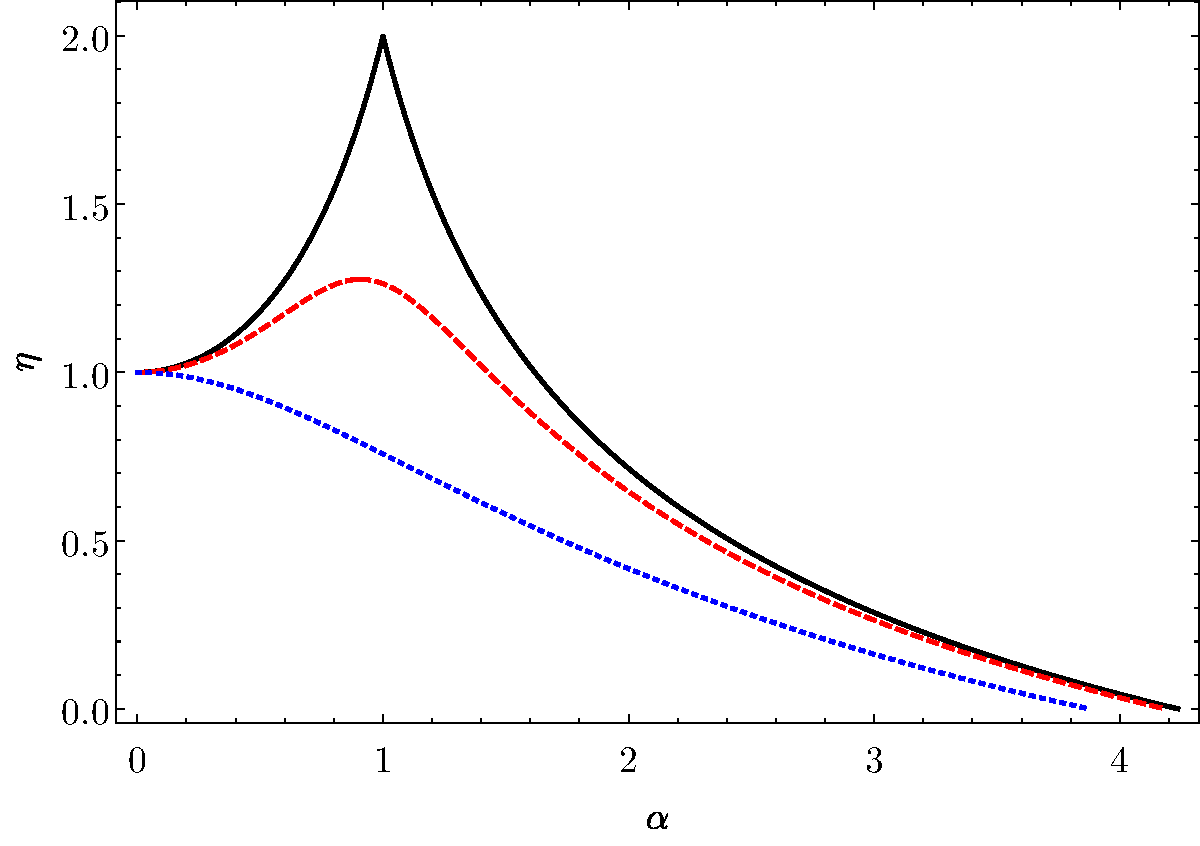
\includegraphics[scale = 0.4]{img/penrose_binaries/mp/efficiency.pdf}
  \caption{Extraction efficiency for a particle $\overline{r} = 1$ and $\overline{\theta} = 0$ (solid black line), $\overline{\theta} = \pi/8$ (dashed red line) and $\overline{\theta} = \pi/2$ (dotted blue line). Maxmimum efficiency is attained at $\alpha = 1$ and $\overline{\theta} = 0,\pi/2$.}
  \label{ch:penrose_binaries/fig:efficiency}
\end{figure}

\section{CMMR spacetime}

We will now perform an analysis similar to that of the previous section but using the solution class found by Cabrera-Munguia, Manko and Ruiz (CMMR). This metric describes a pair of static Kerr black holes and thus we will show that one can extract rotational energy from the system using geodesic motion.

\subsection{Spacetime metric}

In Weyl's cylindrical coordinates, the CMMR line element reads
%
\begin{equation}
  \ud s^2 = -f(\rho,z)\left[\ud t - \omega(\rho,z)\ud\varphi\right]^2 \\
  + f(\rho,z)^{-1}\left[e^{2\gamma(\rho,z)}\left(\ud \rho^2 + \ud z^2\right) + \rho^2\ud\varphi^2\right]
  \label{ch:penrose_binaries/eq:line_element}
\end{equation}
%
where the real valued functions $f(\rho,z)$, $\omega(\rho,z)$ and $\exp[2\gamma(\rho,z)]$ were implemented as described in Sec.~IV of Ref.~\cite{MANKO2020}. We shall not reproduce these functions here as they take a few pages worth of equations.

This solution is characterized by a set five parameters: The masses of the Kerr constituents $m_1$ and $m_2$, their angular momenta per unit mass $a_1$ and $a_2$ and the coordinate distance between the centers of the two black holes $R$. In Weyl's coordinates, each horizon is a line that extends over the $z$ axis centered around $z=\pm R/2$ (See Fig.~3 of Ref.~\cite{MANKO2020}). In order to work with dimensionless quantities, we will introduce the three additional parameters given in terms of the preceding five. The first is the total mass of the system $M$, given by
%
\begin{equation}
  M = m_1 + m_2.
  \label{ch:penrose_binaries/eq:total_mass_def}
\end{equation}
%
The second is the system's mass ratio $q$ given by
%
\begin{equation}
  q = \frac{m_1}{m_2}
  \label{ch:penrose_binaries/eq:mass_ratio_def}
\end{equation}
%
and finally, the third is a dimensionless distance parameter $b$ given by
%
\begin{equation}
  b = \frac{M}{R}.
  \label{ch:penrose_binaries/eq:dist_param_def}
\end{equation}

By performing the coordinate transformation
%
\begin{equation}
  x^{\mu} \rightarrow \frac{x^\mu}{M}
  \label{ch:penrose_binaries/eq:coord_transf_dimensionless}
\end{equation}
%
where the $x^\mu$ are the space-time coordinates, we effectively rescale the metric functions $f$, $\omega$ and $e^{2\gamma}$ by a factor of $1/M$ and as a result they become dimensionless quantities with the added benefit that the space-time coordinates $t$, $\rho$, $z$ and $\varphi$ are also dimensionless quantities.

If additionally we fixate $M$ to be unitary, we can fully describe the CMMR metric by specifying four dimensionless parameters $q$, $b$, $a_1$ and $a_2$ from which all necessary quantities appearing in the metric functions can be calculated. Explicitly, we can write the inverse relations
%
\begin{equation}
  m_1 = \frac{Mq}{1+q},
  \label{ch:penrose_binaries/eq:m1_from_q}
\end{equation}
%
\begin{equation}
  m_2 = \frac{M}{1+q}
  \label{ch:penrose_binaries/eq:m2_from_q}
\end{equation}
%
and
\begin{equation}
  R = \frac{M}{b}.
  \label{ch:penrose_binaries/eq:r_from_b}
\end{equation}

The CMMR solution when written in the form given by Ref.~\cite{MANKO2020} can appropriately describe not only a ``standard'' Kerr black hole binary but also extreme and naked Kerr sources, depending on the values chosen for the solution's parameters. In order to study scenarios of greater astrophysical relevance we shall limit ourselves to discussions pertaining only to the black hole sector of the metric which is given by the set of parameters that cause the constituent black holes horizons half lengths (the expressions for $\sigma_1$ and $\sigma_2$ after Eq. (18) of Ref.~\cite{MANKO2020}) to be real valued and greater than zero. By choosing values of $q$ and $b$, we are able to determine which values of $a_1$ and $a_2$ represent black hole binary solutions. The results are presented in Fig.~\ref{ch:penrose_binaries/fig:parameter_space}. For each $q$ and $b$ pair, a blue shape represents the region of $a_1$ and $a_2$ values representing black hole configurations.

\begin{figure}
  \centering
  \subfloat[$b=0.1$, $q=0.1$]{
    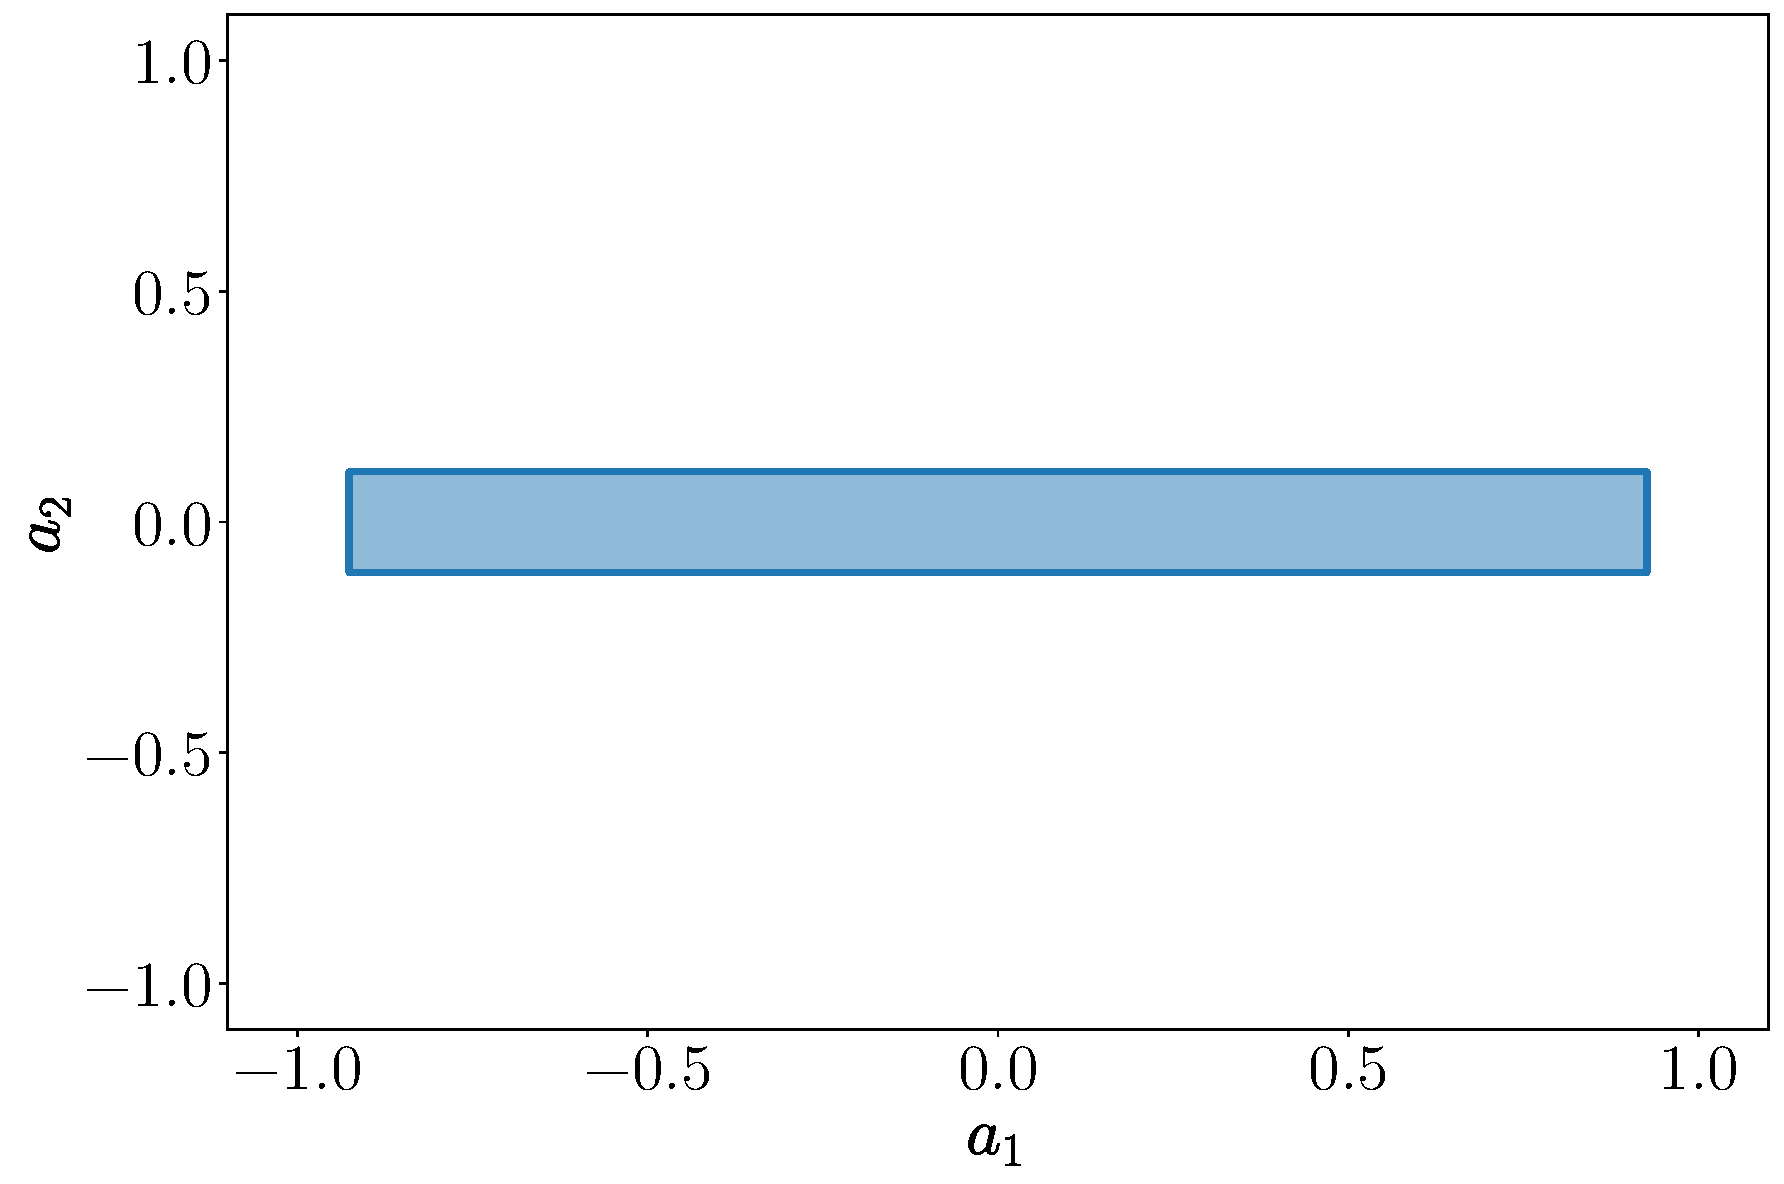
\includegraphics[scale = 0.15]{img/penrose_binaries/cmmr_par_region/par_region_b_0.1_q_0.1.pdf}
    \label{ch:penrose_binaries/fig:par_reg_a}
  }
  \subfloat[$b=0.1$, $q=0.5$]{
    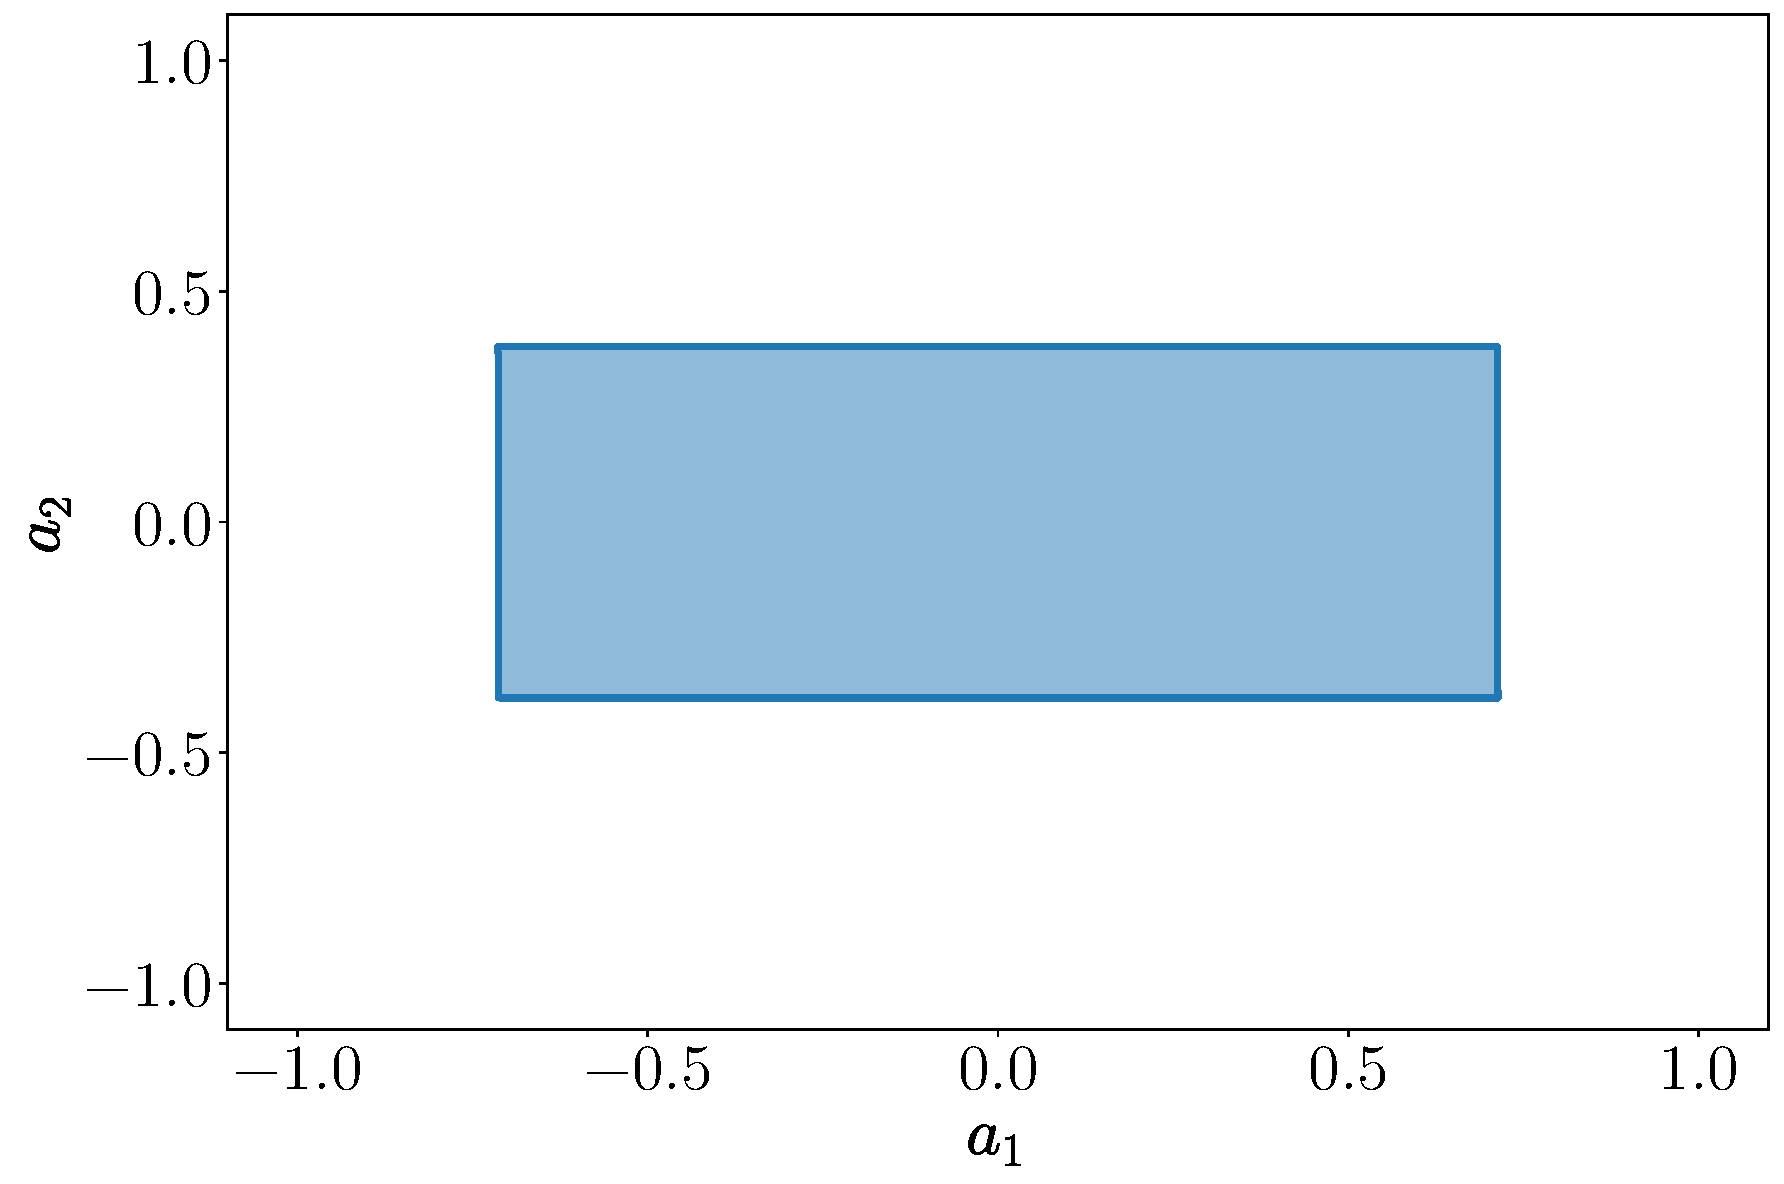
\includegraphics[scale = 0.15]{img/penrose_binaries/cmmr_par_region/par_region_b_0.1_q_0.5.pdf}
    \label{ch:penrose_binaries/fig:par_reg_b}
  }
  \subfloat[$b=0.1$, $q=1.0$]{
    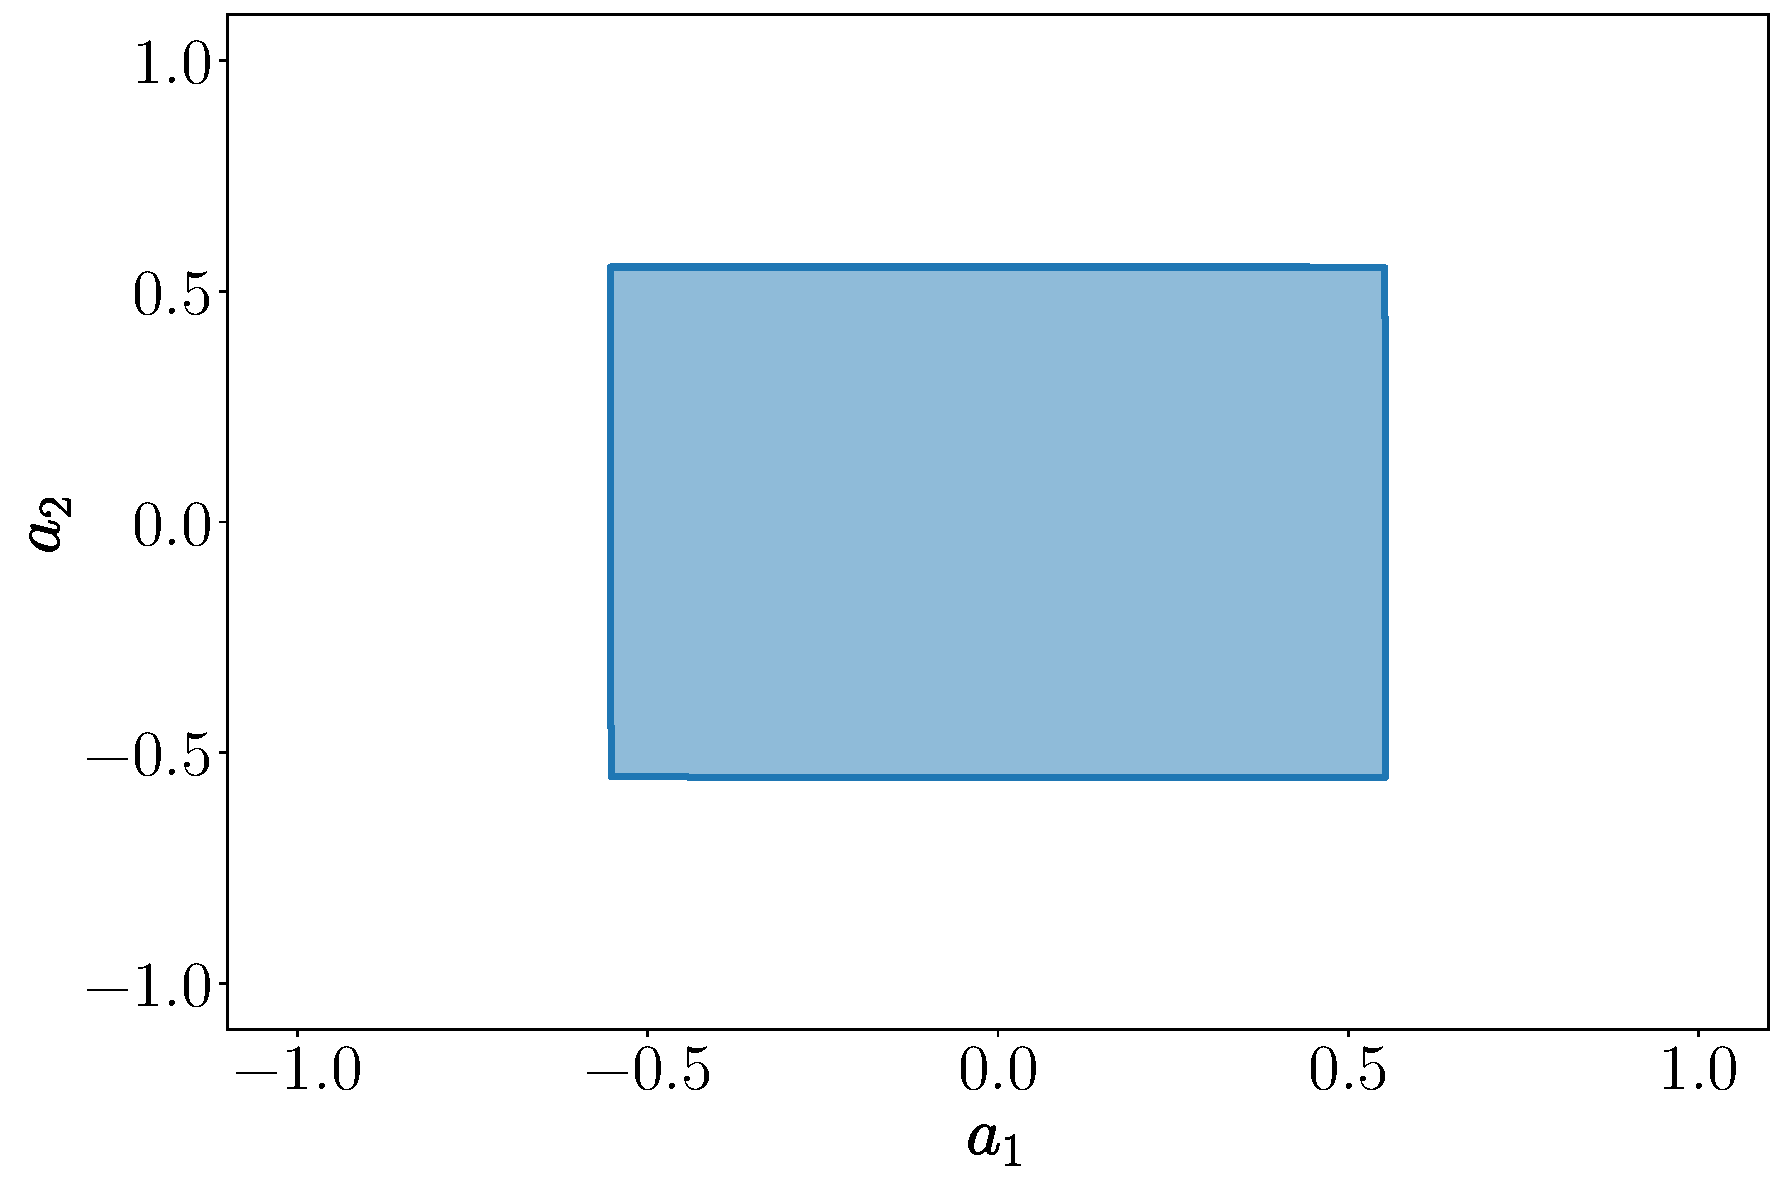
\includegraphics[scale = 0.15]{img/penrose_binaries/cmmr_par_region/par_region_b_0.1_q_1.0.pdf}
    \label{ch:penrose_binaries/fig:par_reg_c}
  }
  \newline
  \subfloat[$b=0.5$, $q=0.1$]{
    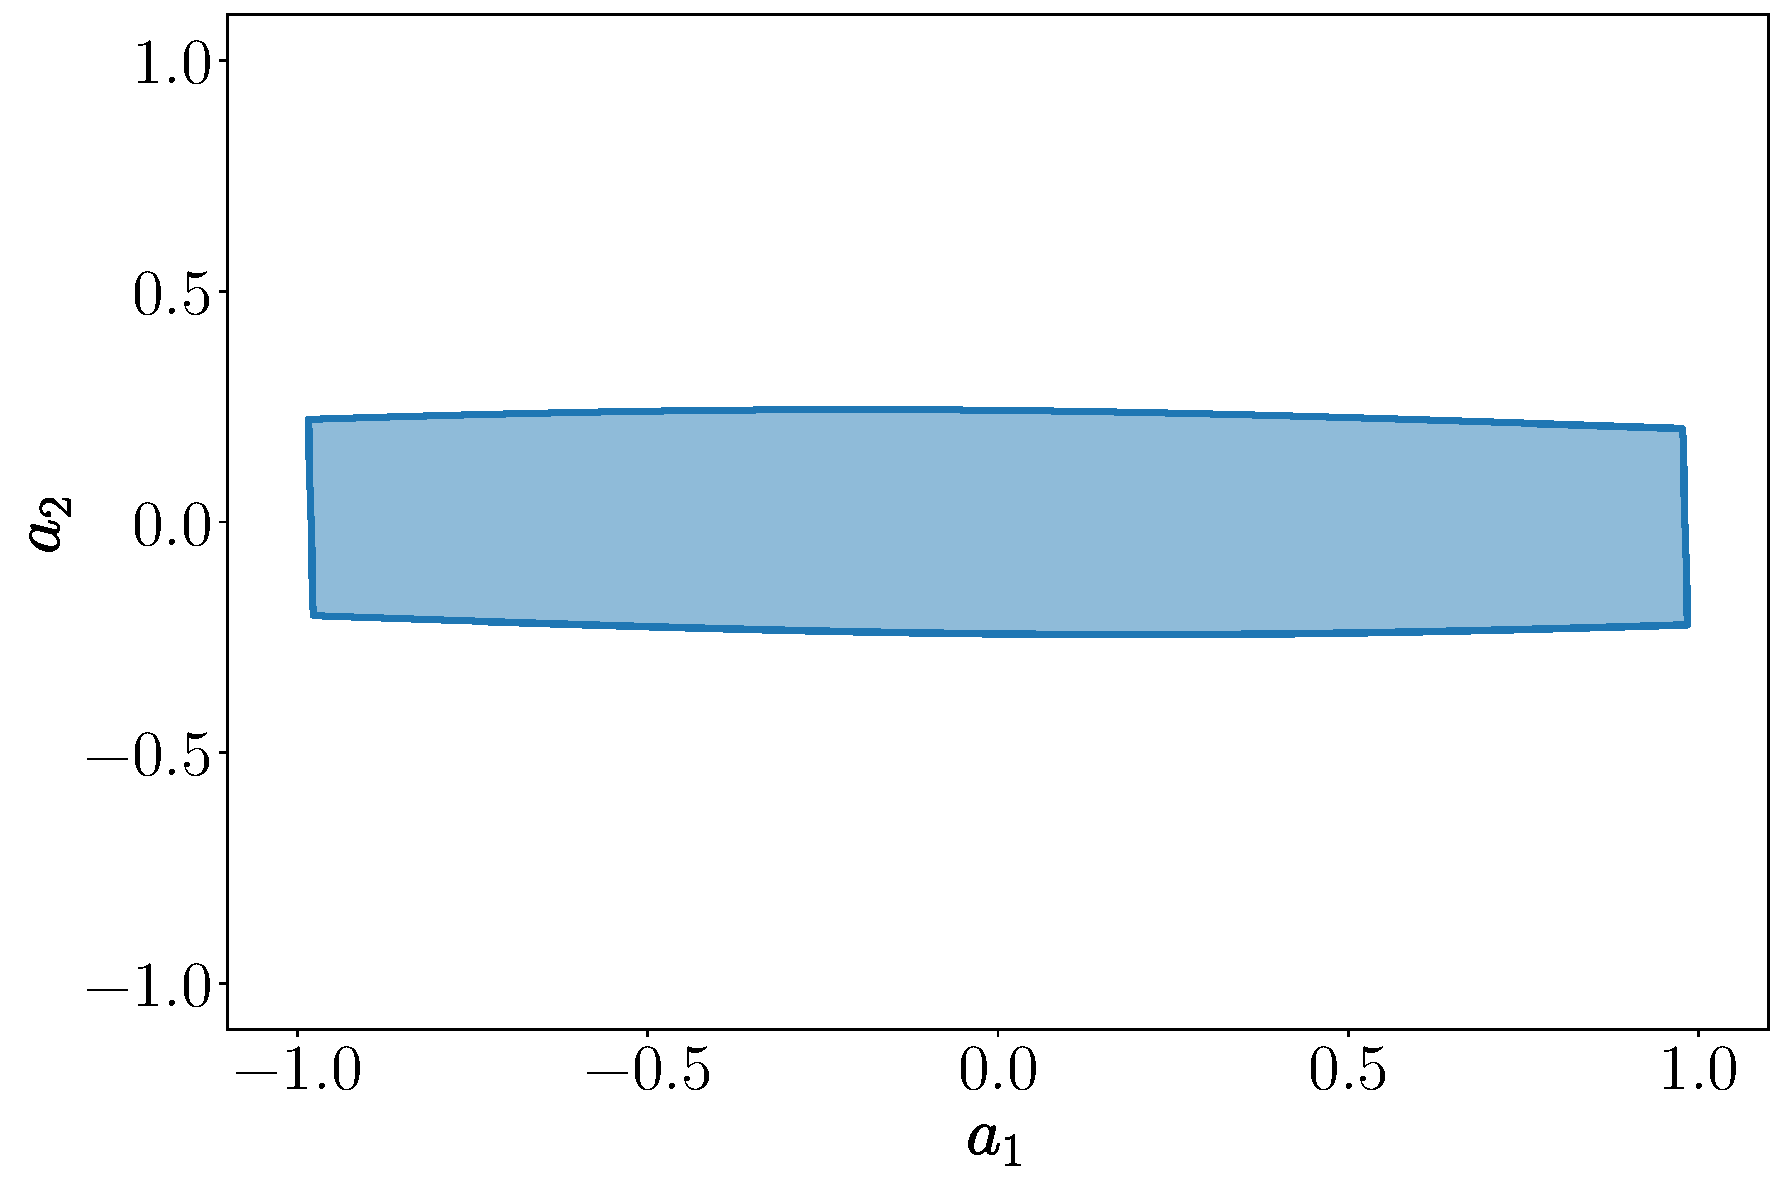
\includegraphics[scale = 0.15]{img/penrose_binaries/cmmr_par_region/par_region_b_0.5_q_0.1.pdf}
    \label{ch:penrose_binaries/fig:par_reg_d}
  }
  \subfloat[$b=0.5$, $q=0.5$]{
    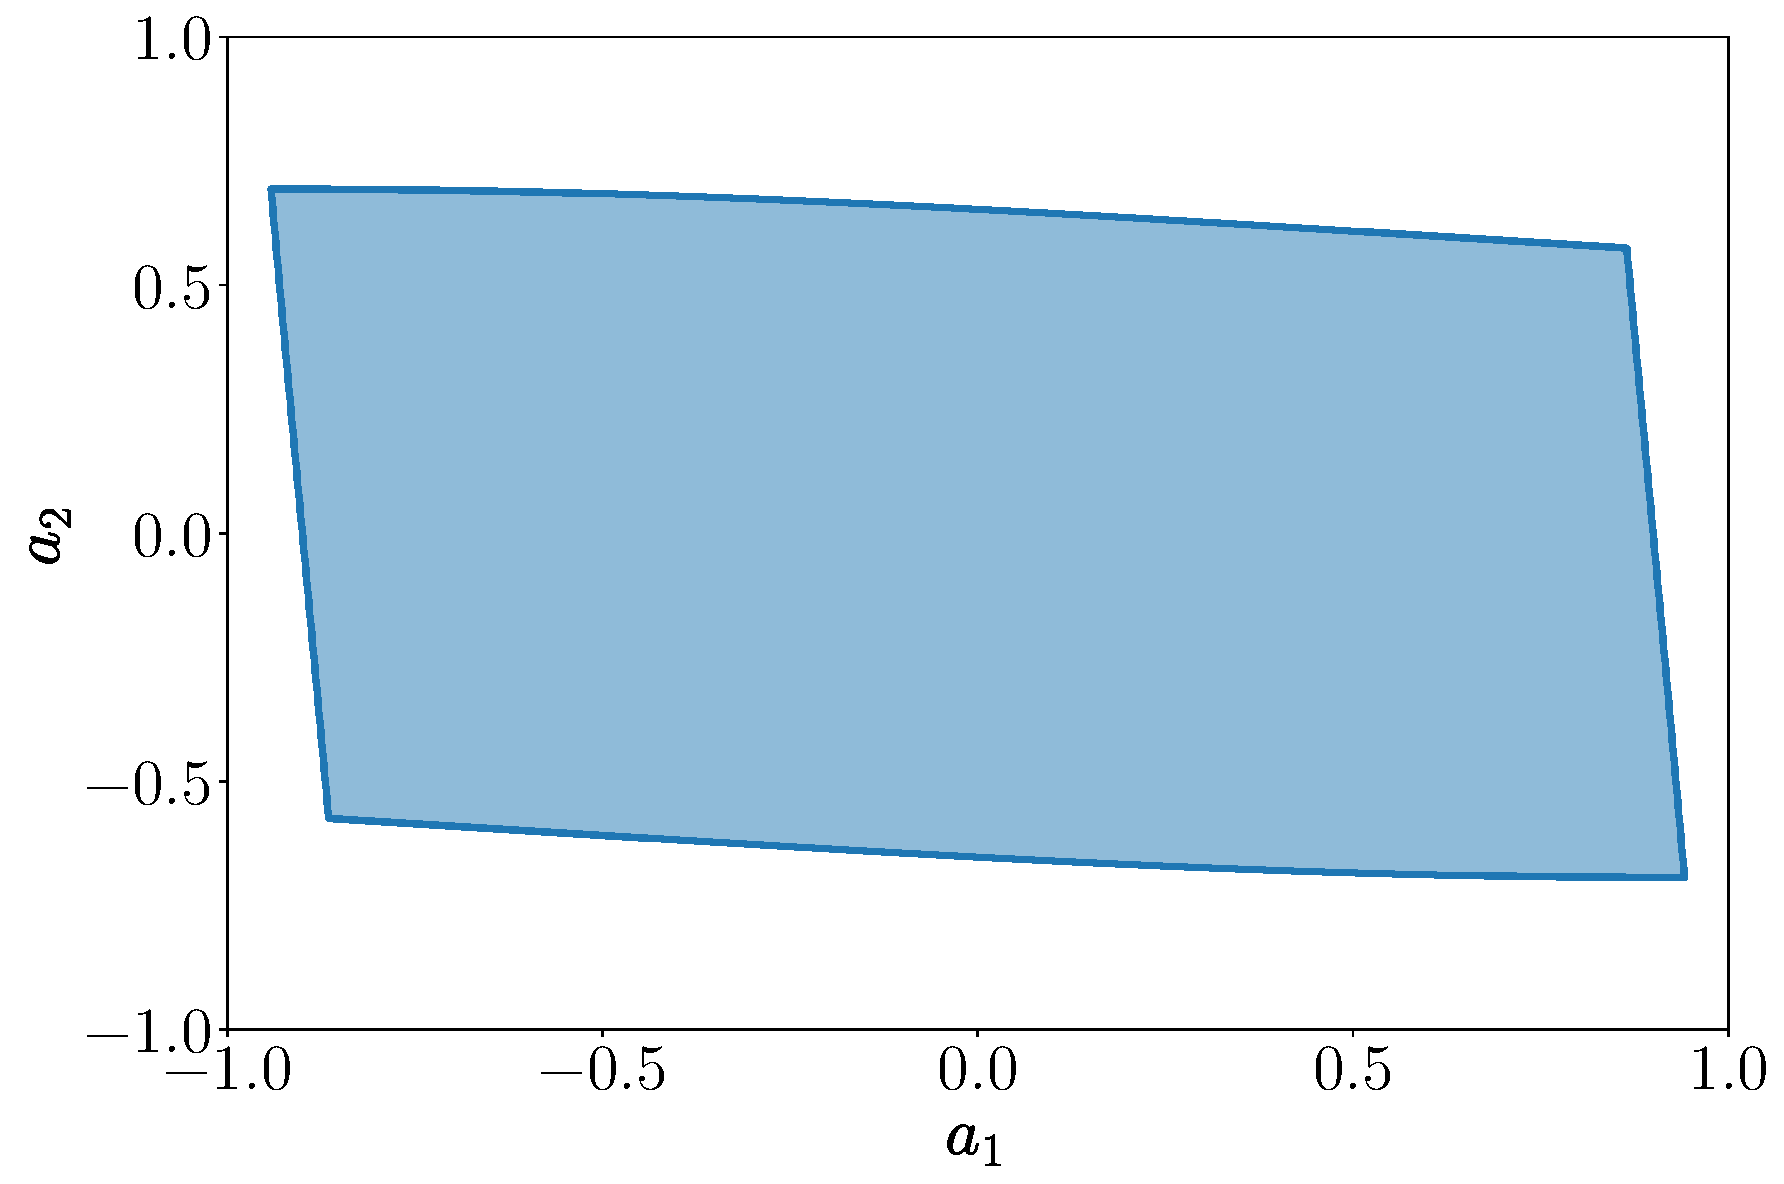
\includegraphics[scale = 0.15]{img/penrose_binaries/cmmr_par_region/par_region_b_0.5_q_0.5.pdf}
    \label{ch:penrose_binaries/fig:par_reg_e}
  }
  \subfloat[$b=0.5$, $q=1.0$]{
    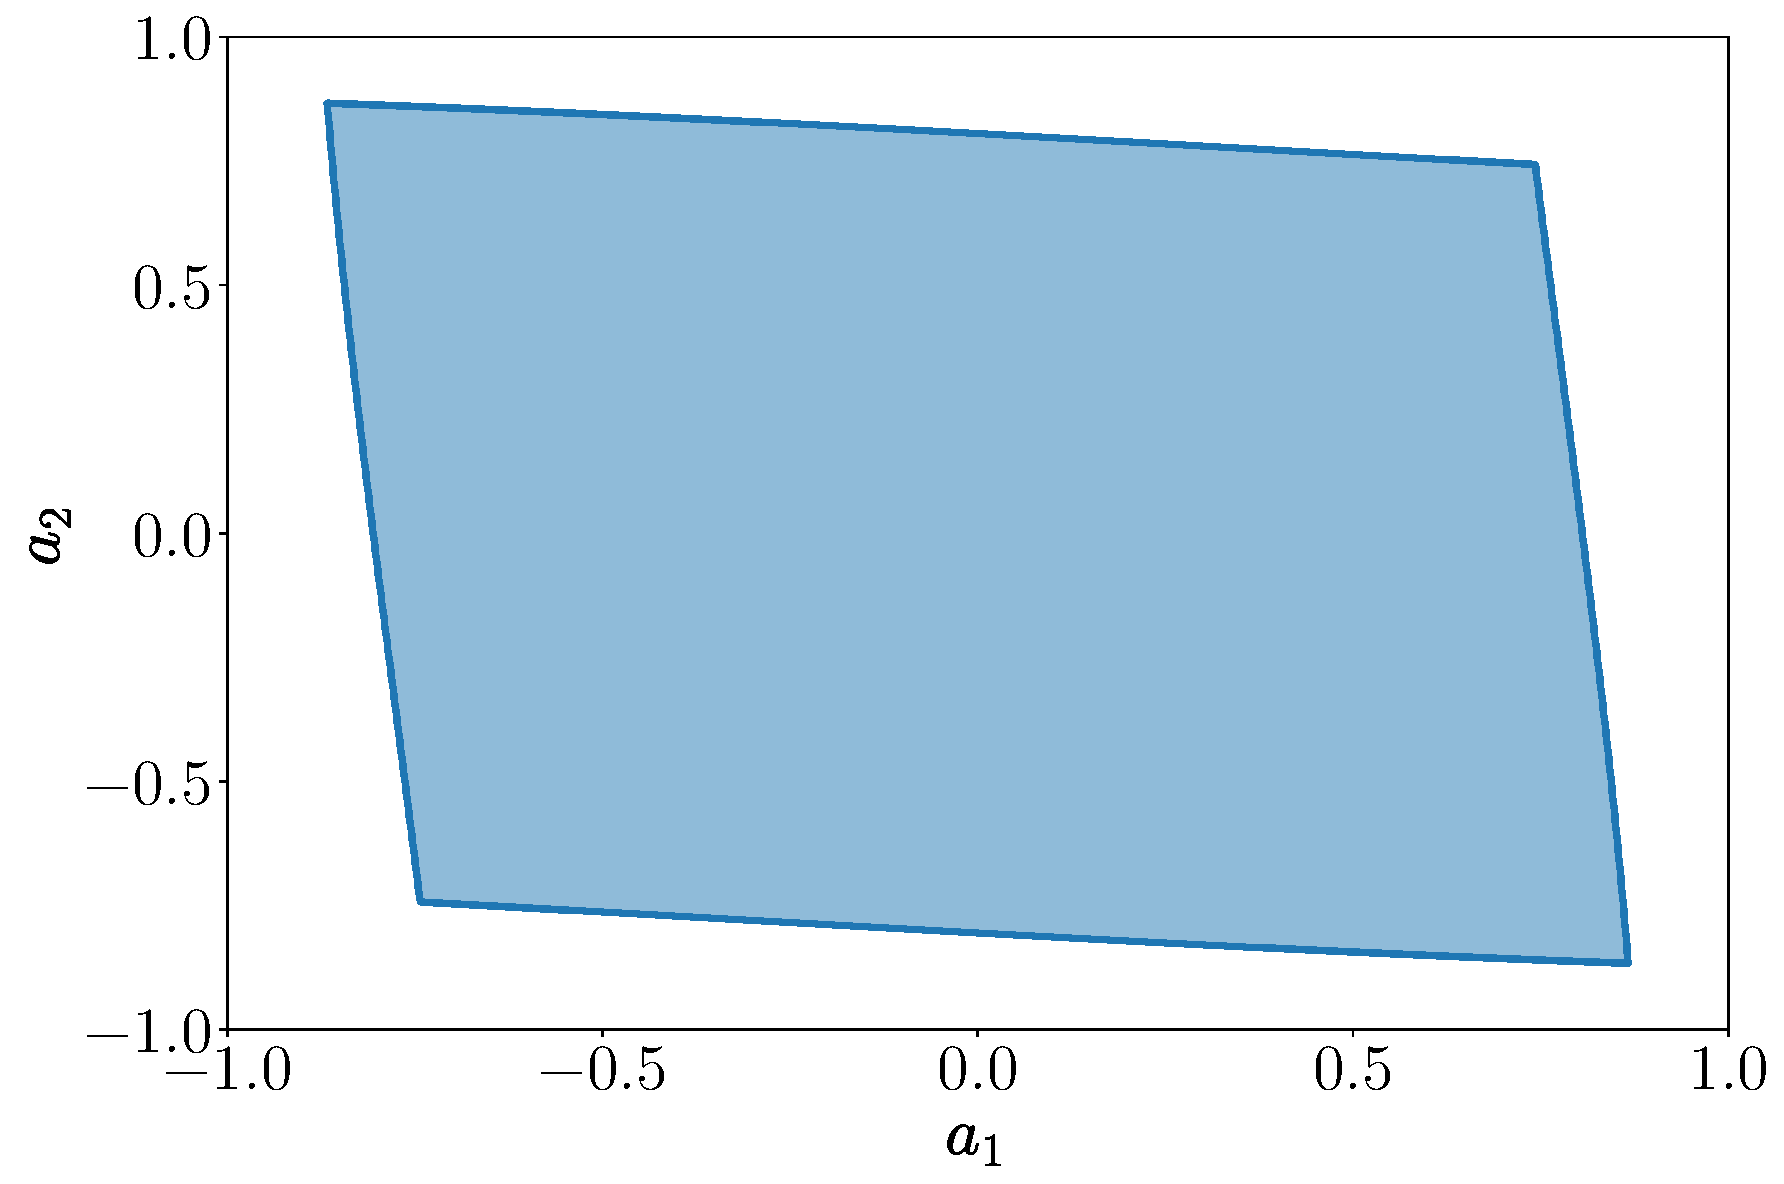
\includegraphics[scale = 0.15]{img/penrose_binaries/cmmr_par_region/par_region_b_0.5_q_1.0.pdf}
    \label{ch:penrose_binaries/fig:par_reg_f}
  }
  \newline
  \subfloat[$b=0.98$, $q=0.1$]{
    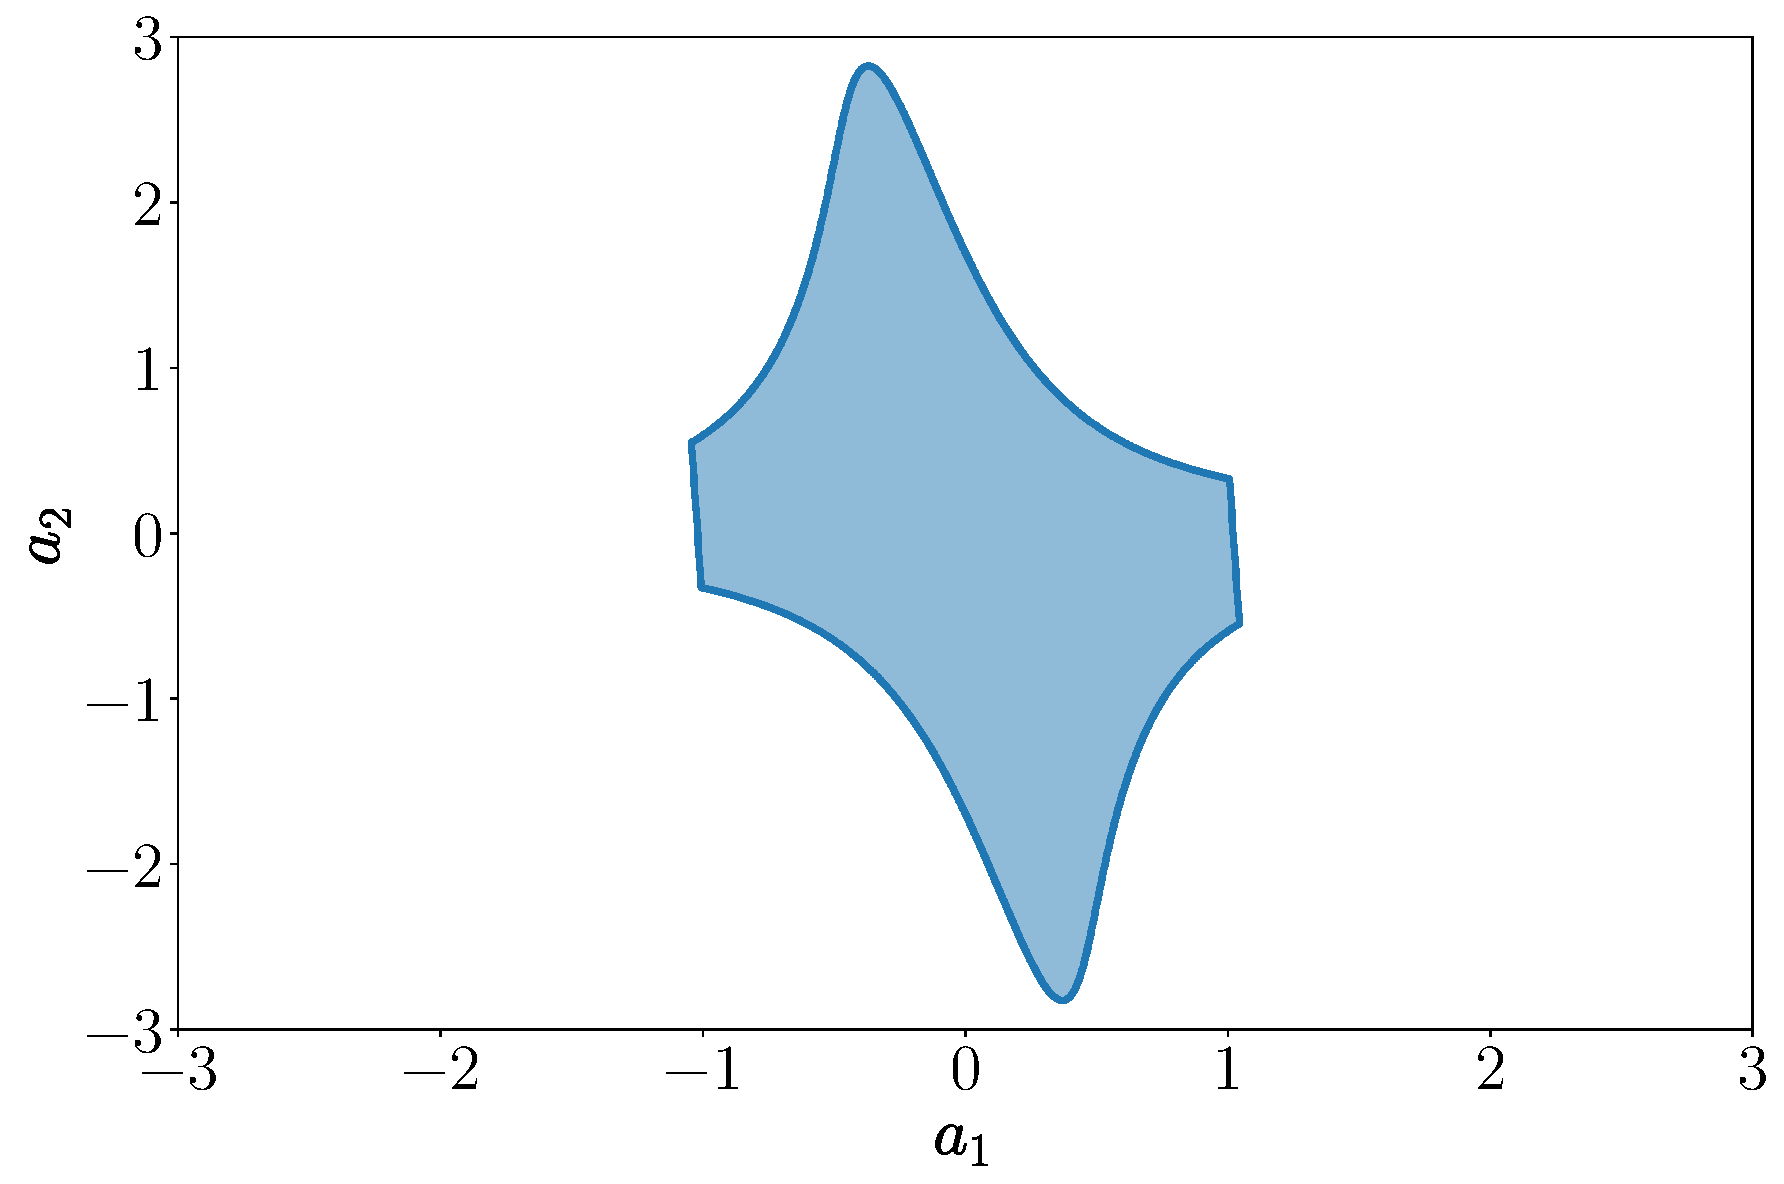
\includegraphics[scale = 0.15]{img/penrose_binaries/cmmr_par_region/par_region_b_0.98_q_0.1.pdf}
    \label{ch:penrose_binaries/fig:par_reg_g}
  }
  \subfloat[$b=0.98$, $q=0.5$]{
    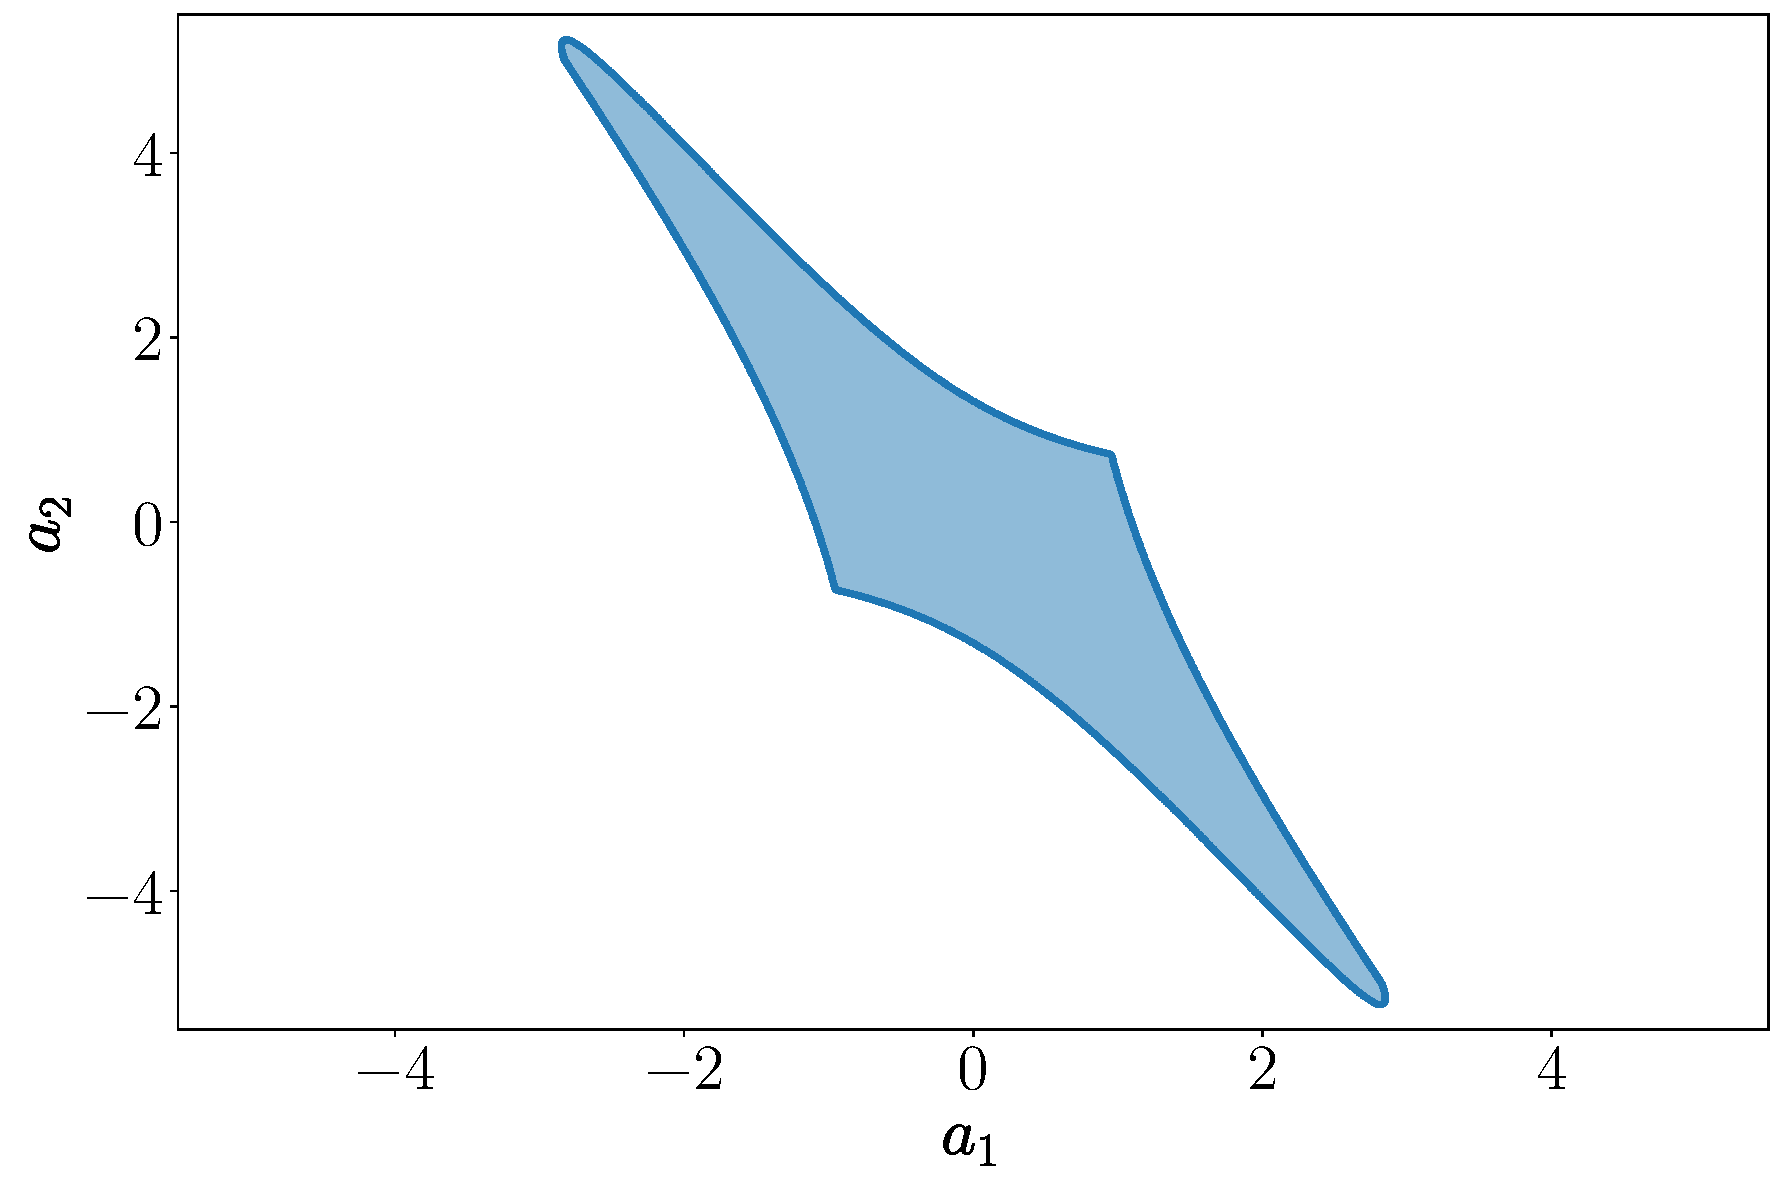
\includegraphics[scale = 0.15]{img/penrose_binaries/cmmr_par_region/par_region_b_0.98_q_0.5.pdf}
    \label{ch:penrose_binaries/fig:par_reg_h}
  }
  \subfloat[$b=0.98$, $q=1.0$]{
    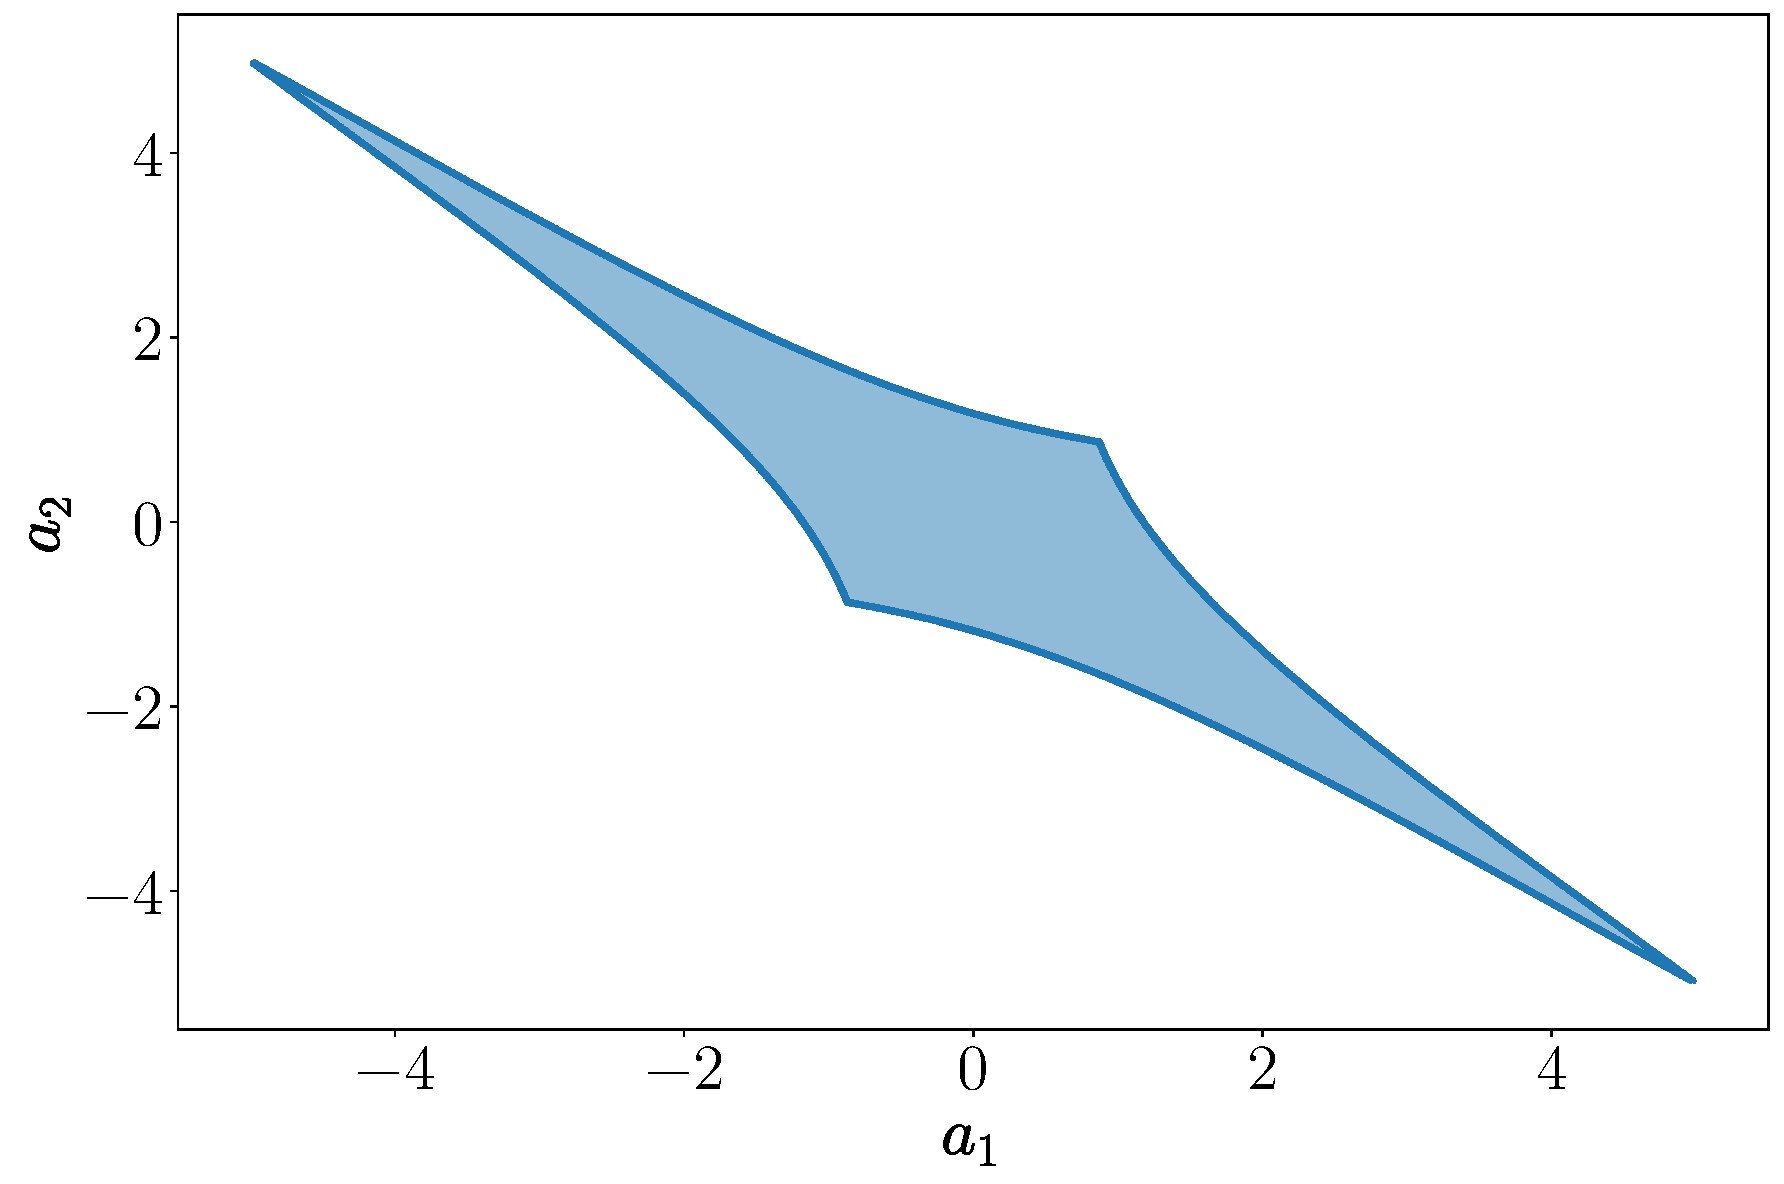
\includegraphics[scale = 0.15]{img/penrose_binaries/cmmr_par_region/par_region_b_0.98_q_1.0.pdf}
    \label{ch:penrose_binaries/fig:par_reg_i}
  }
  \caption{Parameter space variations in the CMMR solution. All $a_1$ and $a_2$ values inside of the blue region represent a valid black hole binary solution for a set of indicated $q$ and $b$ values.}
  \label{ch:penrose_binaries/fig:parameter_space}
\end{figure}

\subsection{Ergospheres}

In the context of stationary space-times the ergosphere is defined as the region in which observers can no longer be static and are ``dragged'' along the space-time's rotation. More precisely it is the region in which the time translation Killing vector field $K = \partial_t$ becomes space-like, that is, $\mtrtens{\mu}{\nu}\tens{K}{\mu}{}\tens{K}{\nu}{} >0$~\cite{CARROLL}. In the specific case of the CMMR metric, by employing Eq.~\eqref{ch:penrose_binaries/eq:line_element} we see that the ergosphere is the locus of all points $(\rho,z)$ that satisfy
%
\begin{equation}
  f(\rho,z) < 0.
  \label{ch:penrose_binaries/eq:ergosphere_def}
\end{equation}

Given the complexity of $f(\rho,z)$ it is extremely difficult (or even impossible) to find an explicit expression for $\rho$ and $z$ that satisfy Eq.~\eqref{ch:penrose_binaries/eq:ergosphere_def} thus we will visualize the ergospheres and their features in the CMMR solution numerically. Knowing that the relation between Weyl's radial coordinate $\rho$ and Cartesian coordinates $x$ and $y$ are $x = \rho\cos\varphi$ and $y = \rho\sin\varphi$ we can project and plot $f(\rho,z)$ in the $x$-$z$ plane by choosing $\varphi=0$.

To create the plots, we have fixed $q = 1.0$ and $|a_{1,2}| = 0.65$ while gradually increased $b$ from $0.3$ to $0.98$. This allows us to view the ergosphere around each constituent of the binary changing as their mutual interaction grows stronger. In Fig.~\ref{ch:penrose_binaries/fig:ergo_equal_spin} we show the variation of the ergosphere for constituents of aligned spins and in Fig.~\ref{ch:penrose_binaries/fig:ergo_unequal_spin} for constituents with anti-aligned spins. In all of the figures the ergosphere is the light blue region, bounded by the darker blue line and the event horizons are black lines. In both cases, the ergospheres start localized around each black hole. The choice of parameters in the figures intentionally lead to horizons that are initially very short which means that the black hole are spinning close to extremality.

\begin{figure}
  \centering
  \subfloat[$b=0.3$]{
    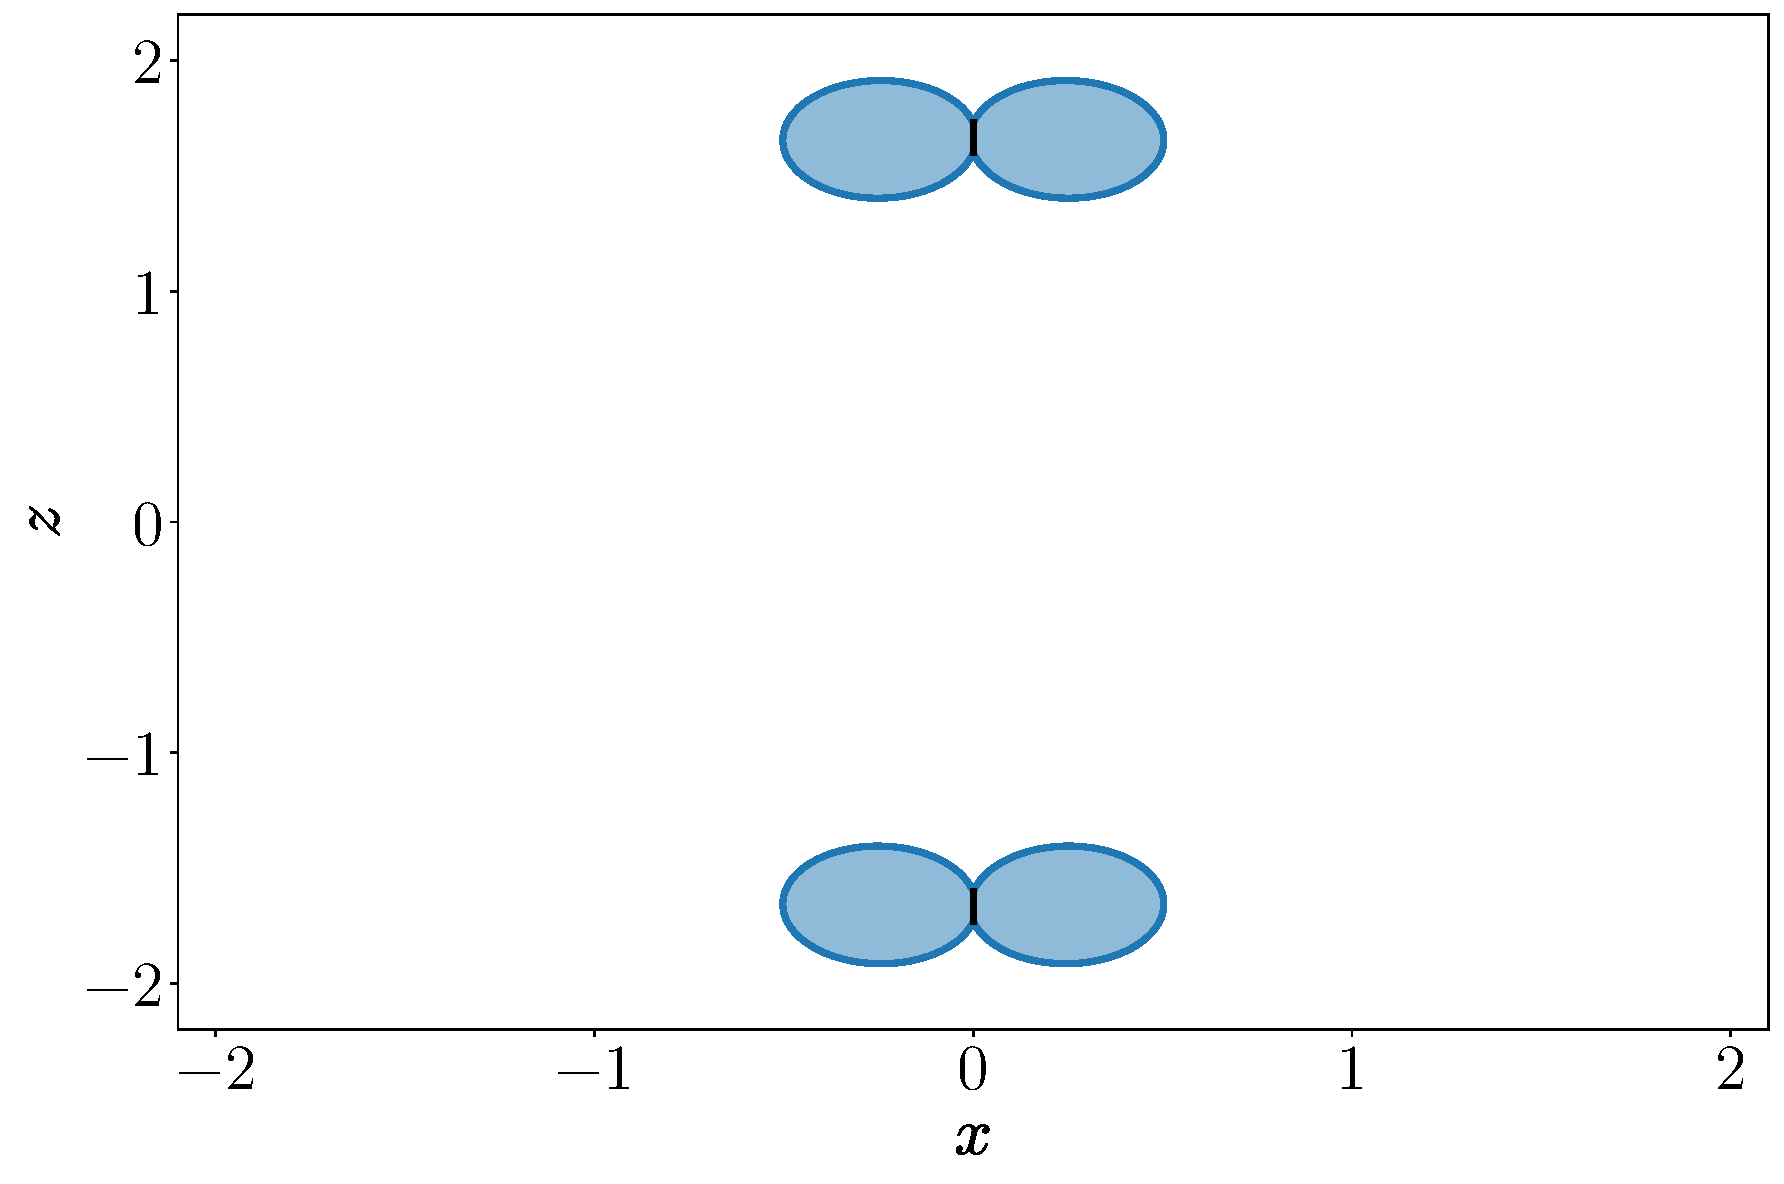
\includegraphics[scale = 0.22]{img/penrose_binaries/cmmr_ergo/ergo_b_0.3_q_1.0_a1_0.65_a2_0.65.pdf}
    \label{ch:penrose_binaries/fig:ergo_equal_a}
  }
  \subfloat[$b=0.5$]{
    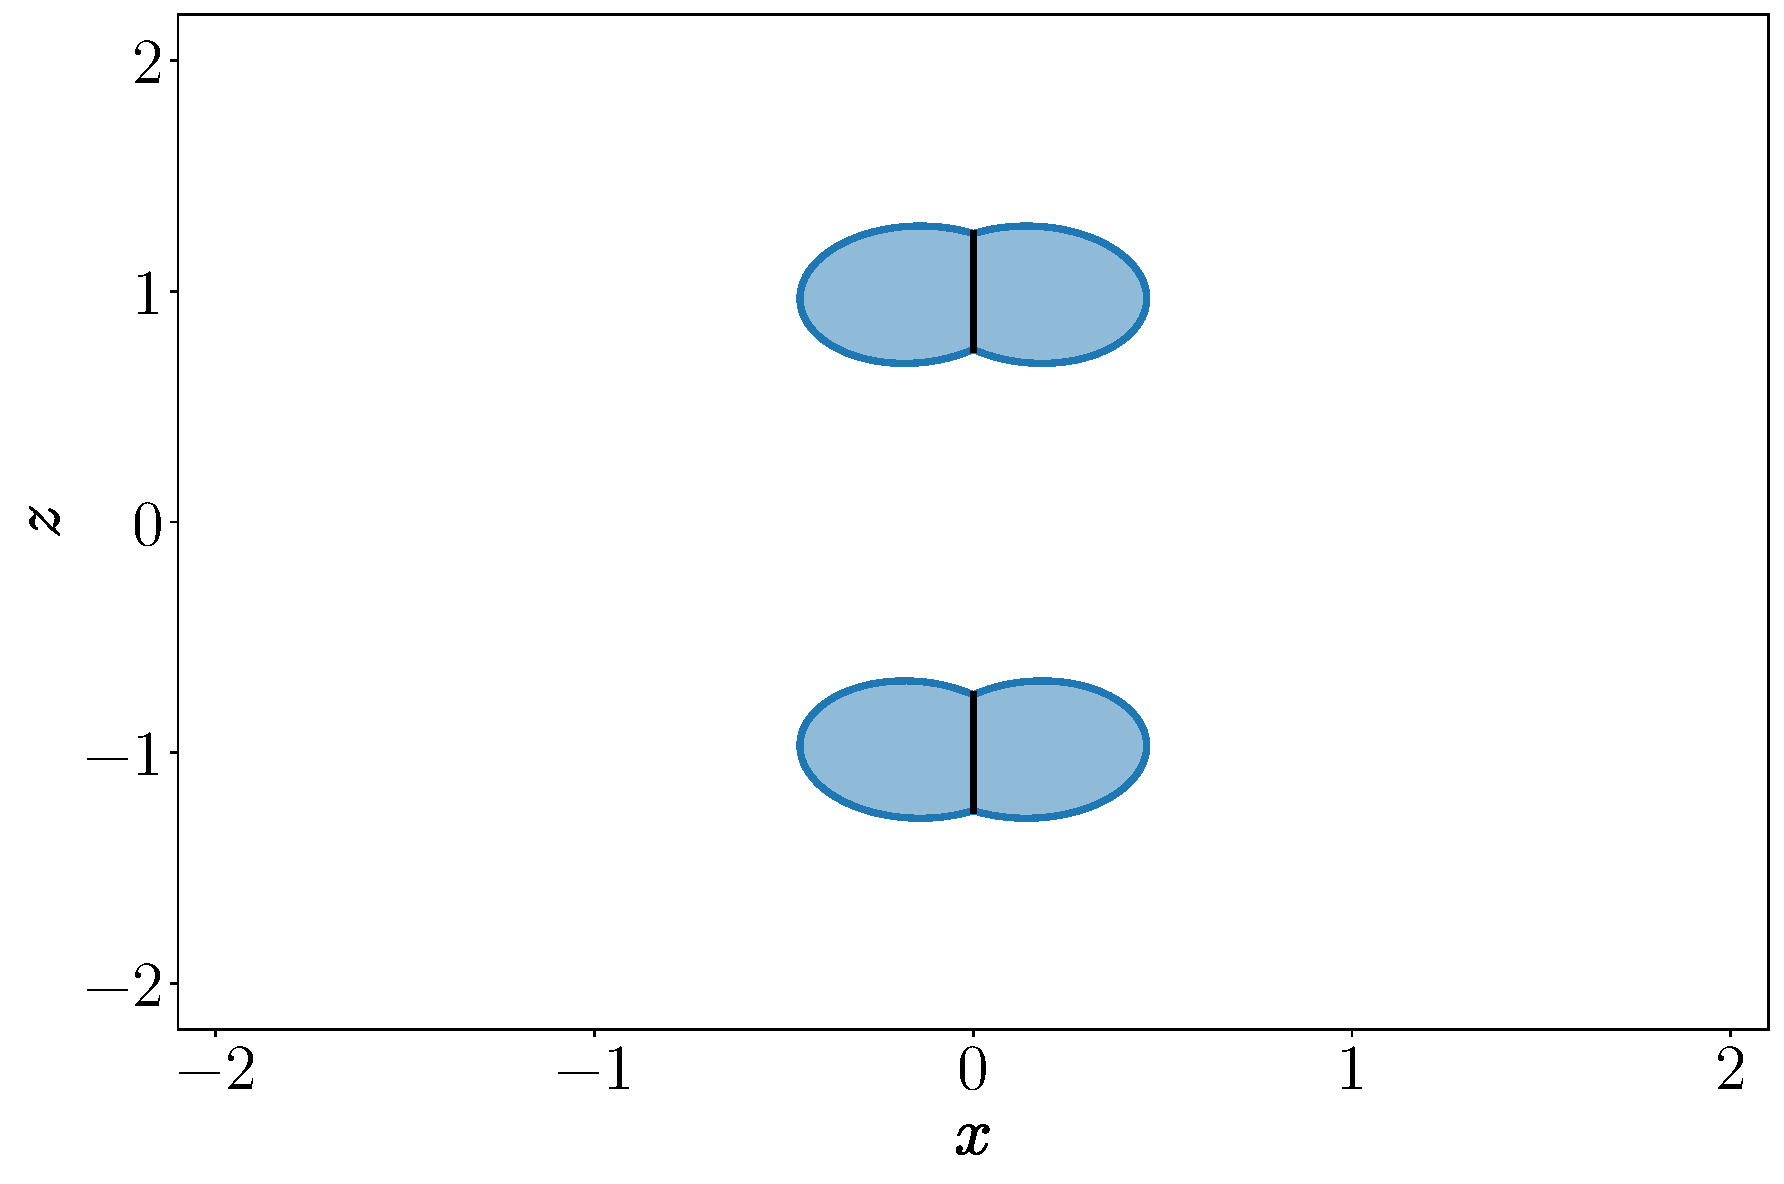
\includegraphics[scale = 0.22]{img/penrose_binaries/cmmr_ergo/ergo_b_0.5_q_1.0_a1_0.65_a2_0.65.pdf}
    \label{ch:penrose_binaries/fig:ergo_equal_b}
  }
  \newline
  \subfloat[$b=0.7$]{
    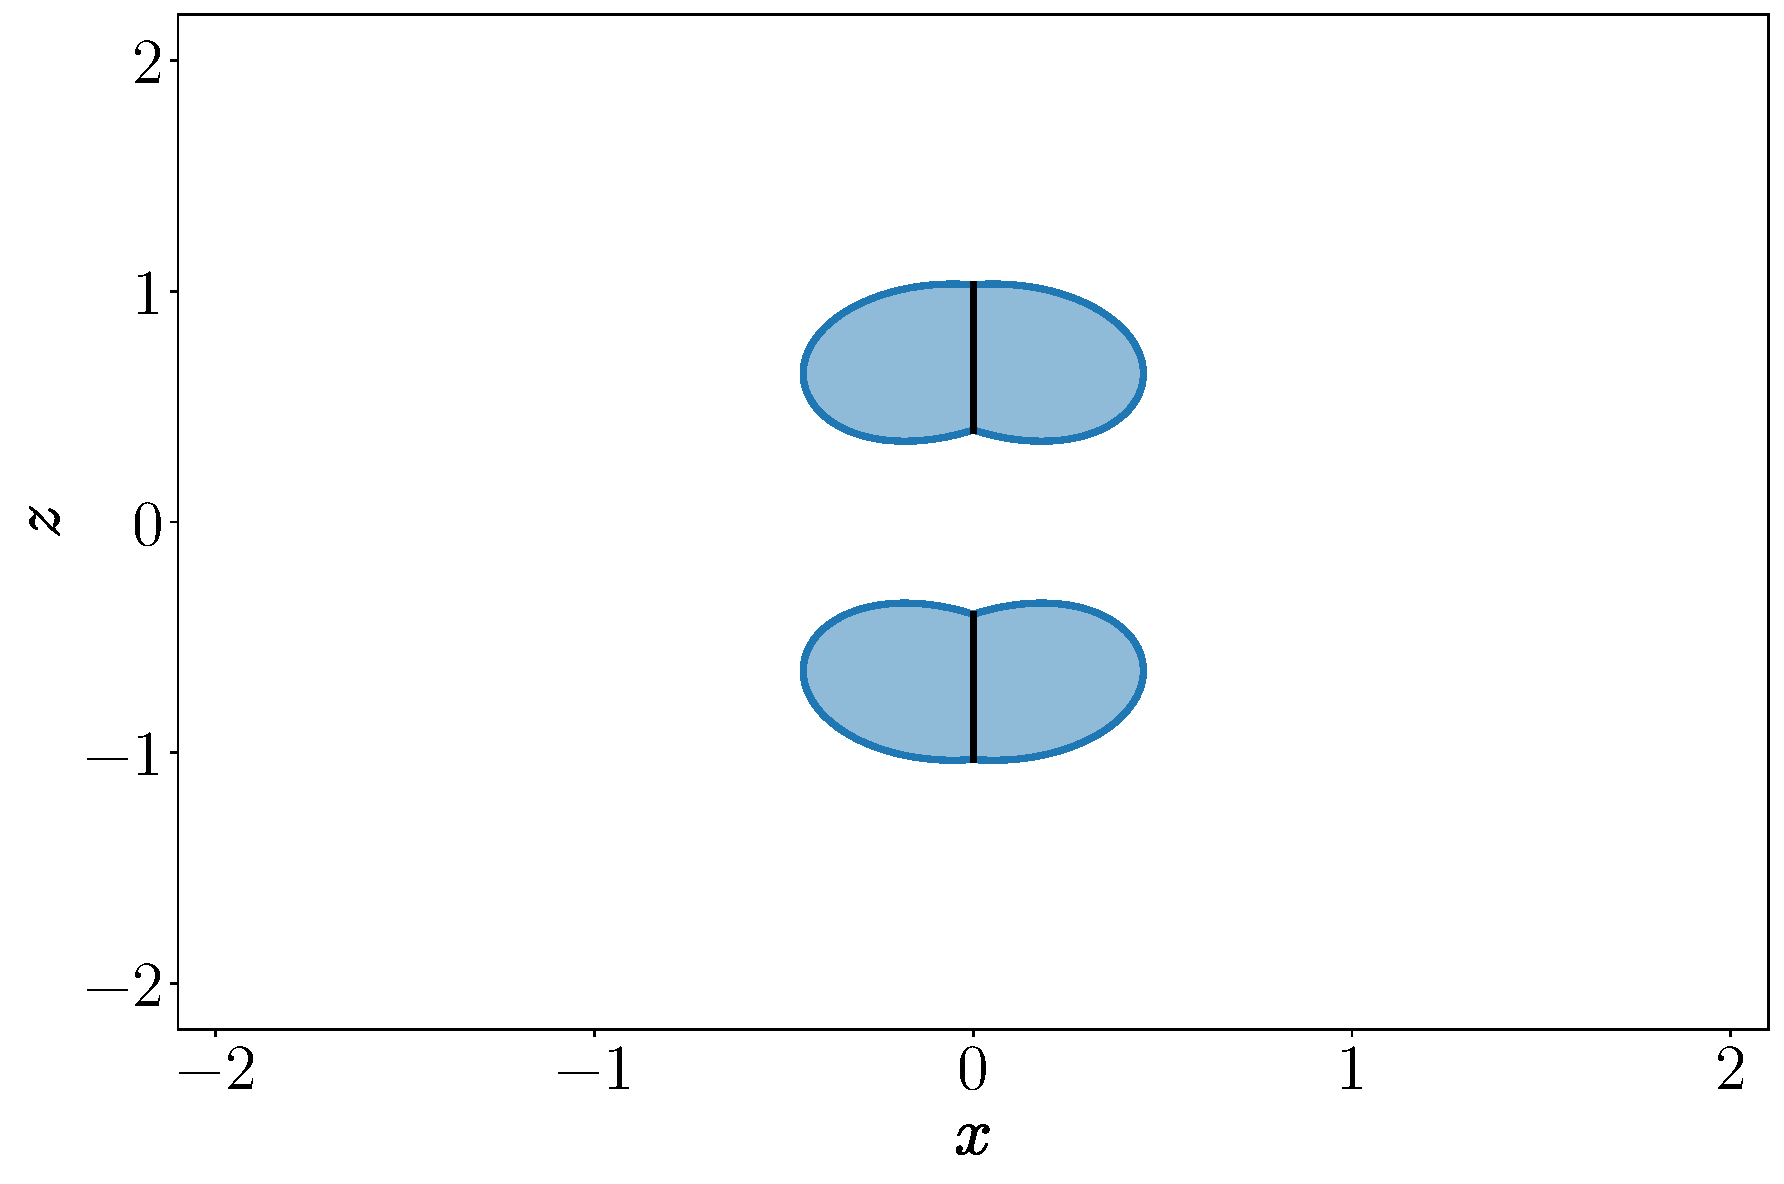
\includegraphics[scale = 0.22]{img/penrose_binaries/cmmr_ergo/ergo_b_0.7_q_1.0_a1_0.65_a2_0.65.pdf}
    \label{ch:penrose_binaries/fig:ergo_equal_c}
  }
  \subfloat[$b=0.98$]{
    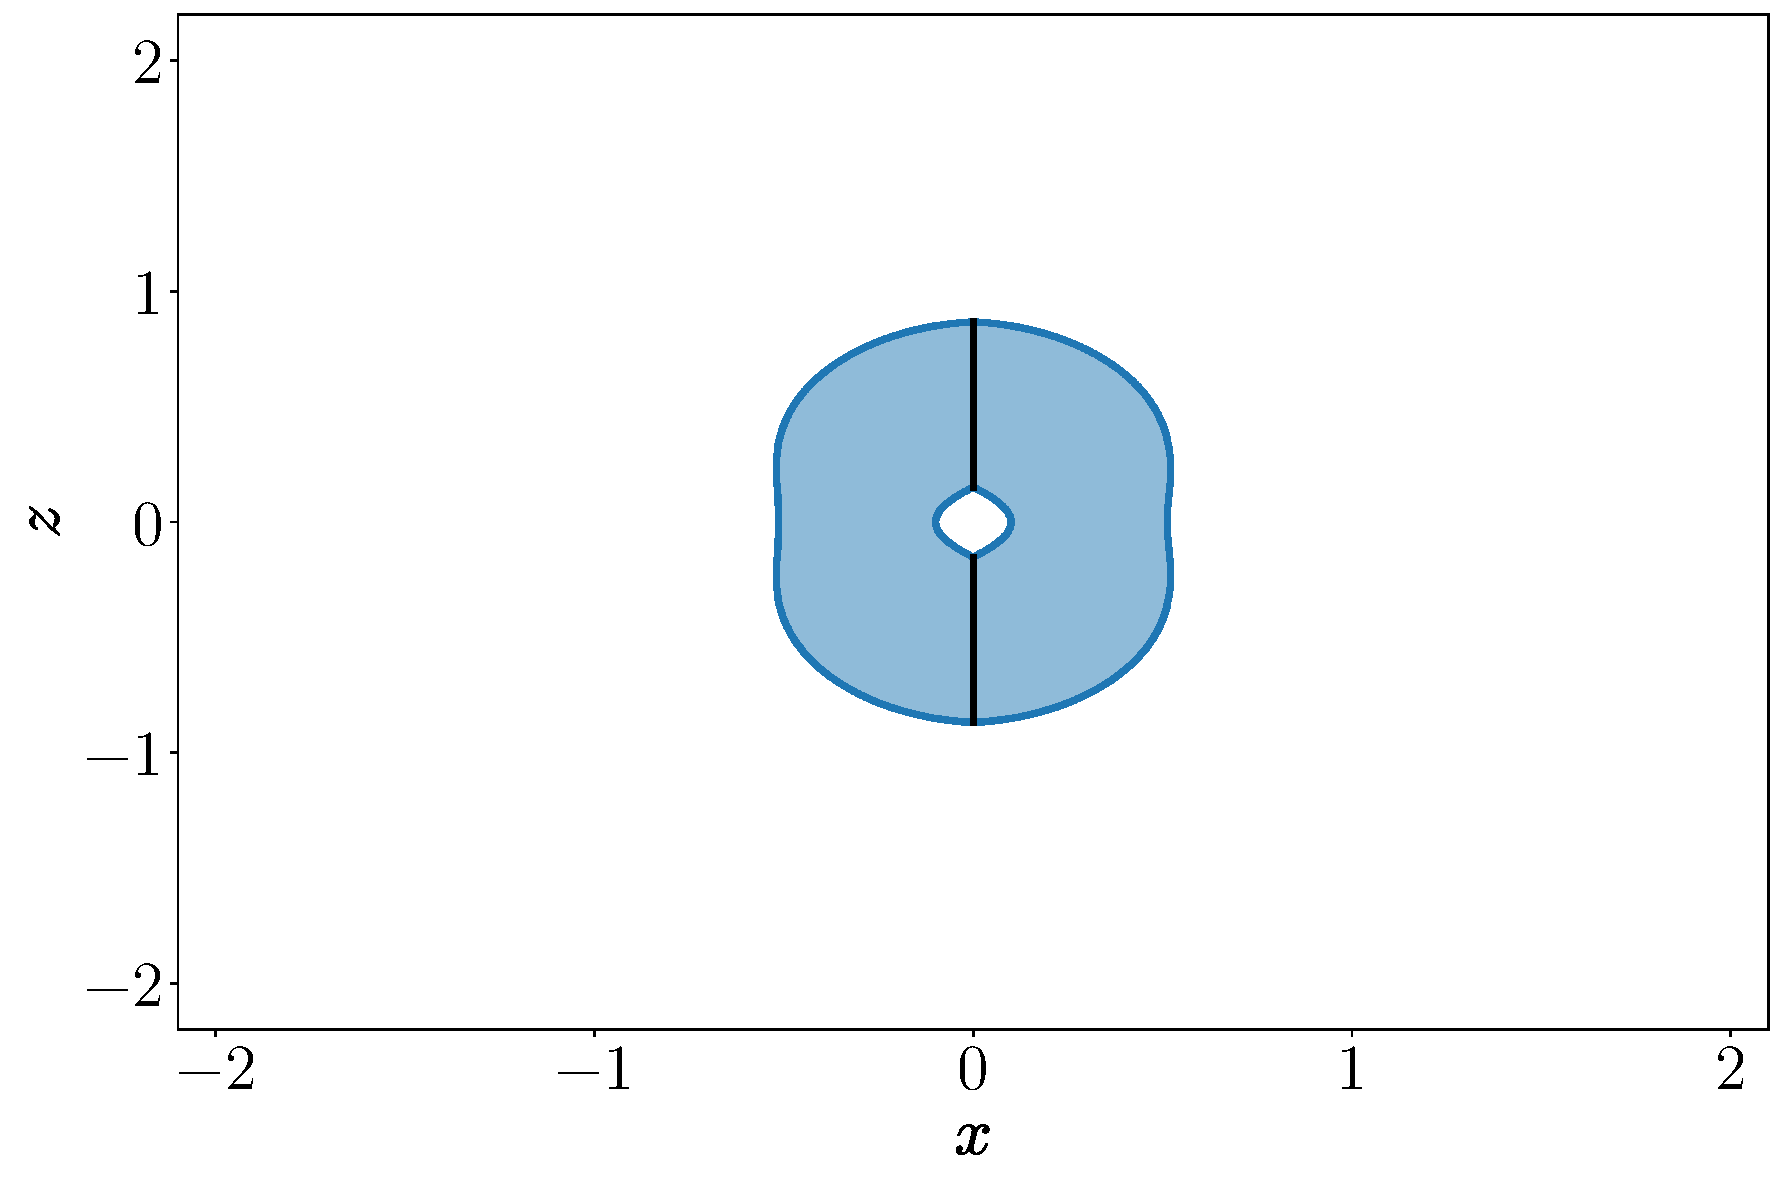
\includegraphics[scale = 0.22]{img/penrose_binaries/cmmr_ergo/ergo_b_0.98_q_1.0_a1_0.65_a2_0.65.pdf}
    \label{ch:penrose_binaries/fig:ergo_equal_d}
  }
  \caption{Ergosphere of a binary Kerr black hole system with mass ratio $q=1.0$ and aligned spins $a_1=0.65$ and $a_2=0.65$ for differente separation parameters. The blu region represents the ergosphere while the black lines represent the event horizons.}
  \label{ch:penrose_binaries/fig:ergo_equal_spin}
\end{figure}

\begin{figure}
  \centering
  \subfloat[$b=0.3$]{
    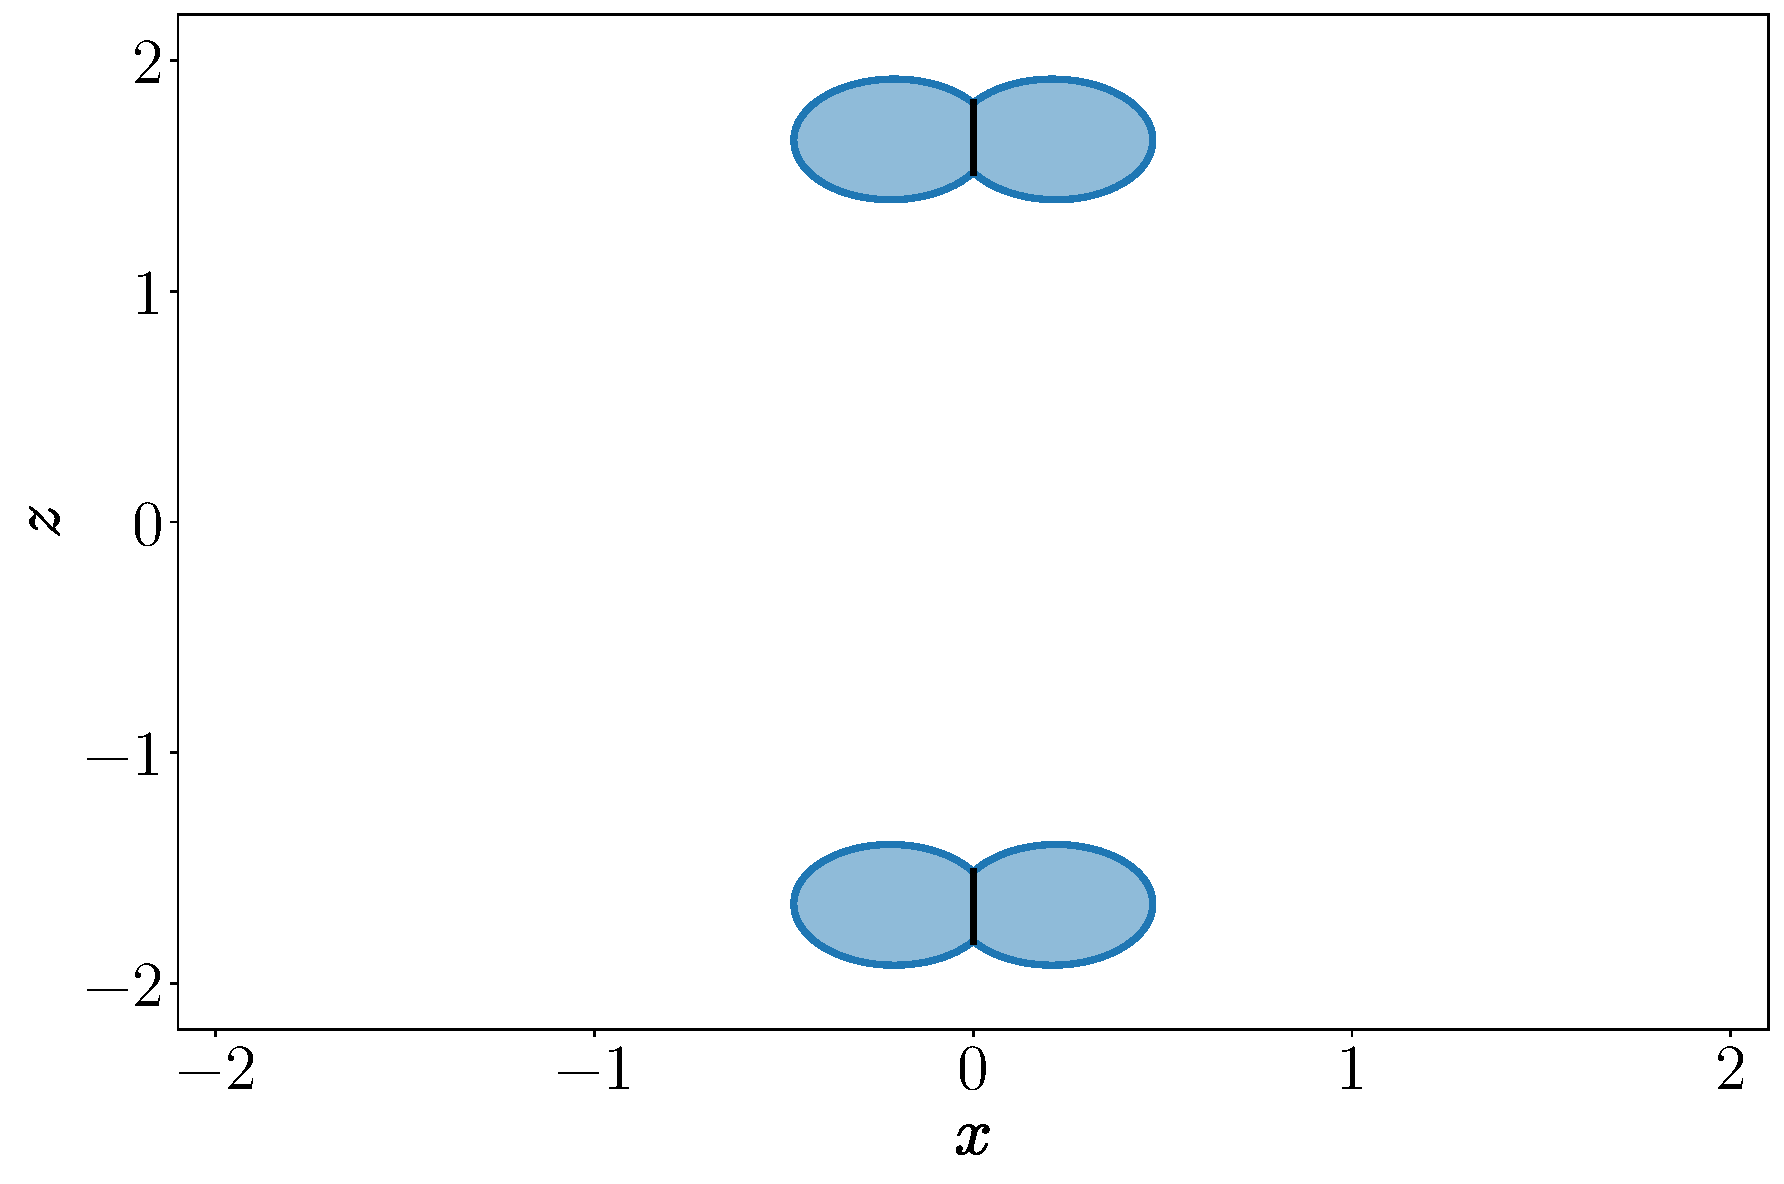
\includegraphics[scale = 0.22]{img/penrose_binaries/cmmr_ergo/ergo_b_0.3_q_1.0_a1_-0.65_a2_0.65.pdf}
    \label{ch:penrose_binaries/fig:ergo_unequal_a}
  }
  \subfloat[$b=0.5$]{
    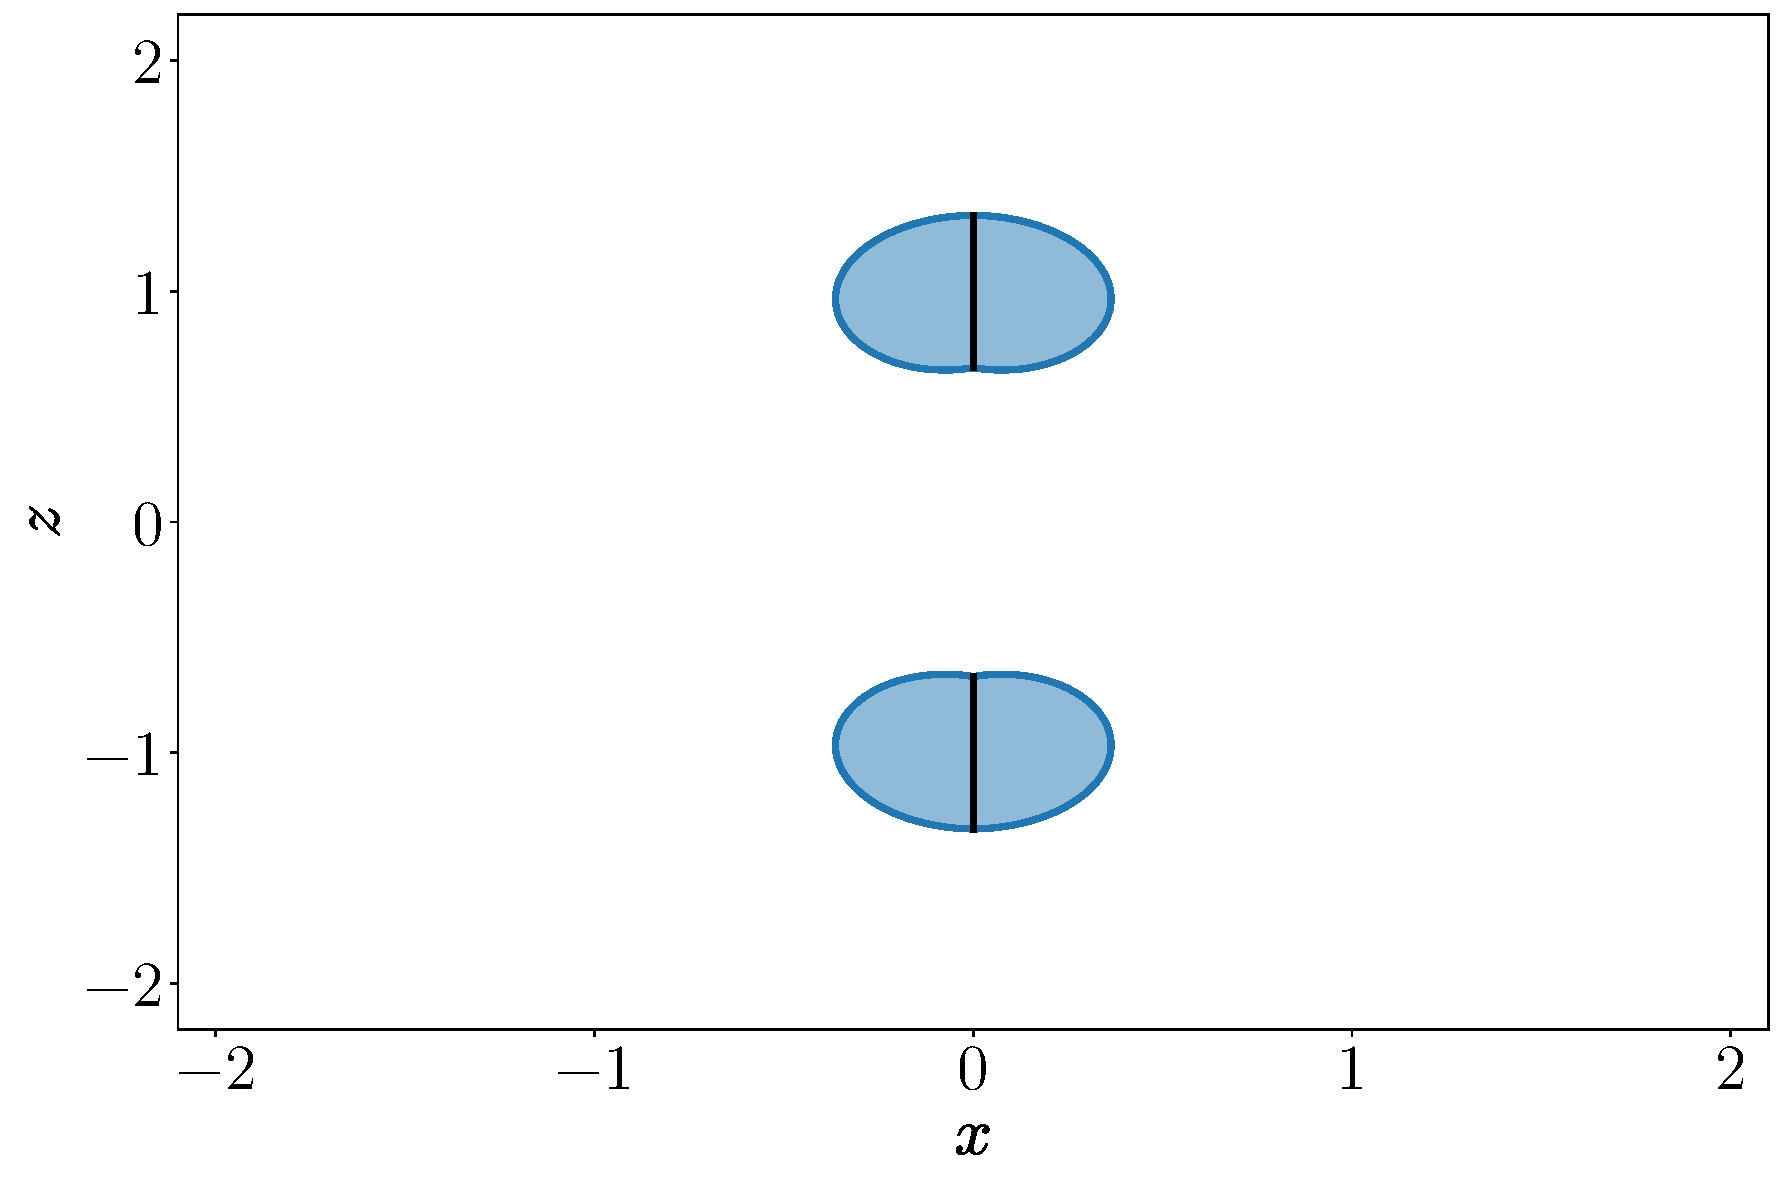
\includegraphics[scale = 0.22]{img/penrose_binaries/cmmr_ergo/ergo_b_0.5_q_1.0_a1_-0.65_a2_0.65.pdf}
    \label{ch:penrose_binaries/fig:ergo_unequal_b}
  }
  \newline
  \subfloat[$b=0.7$]{
    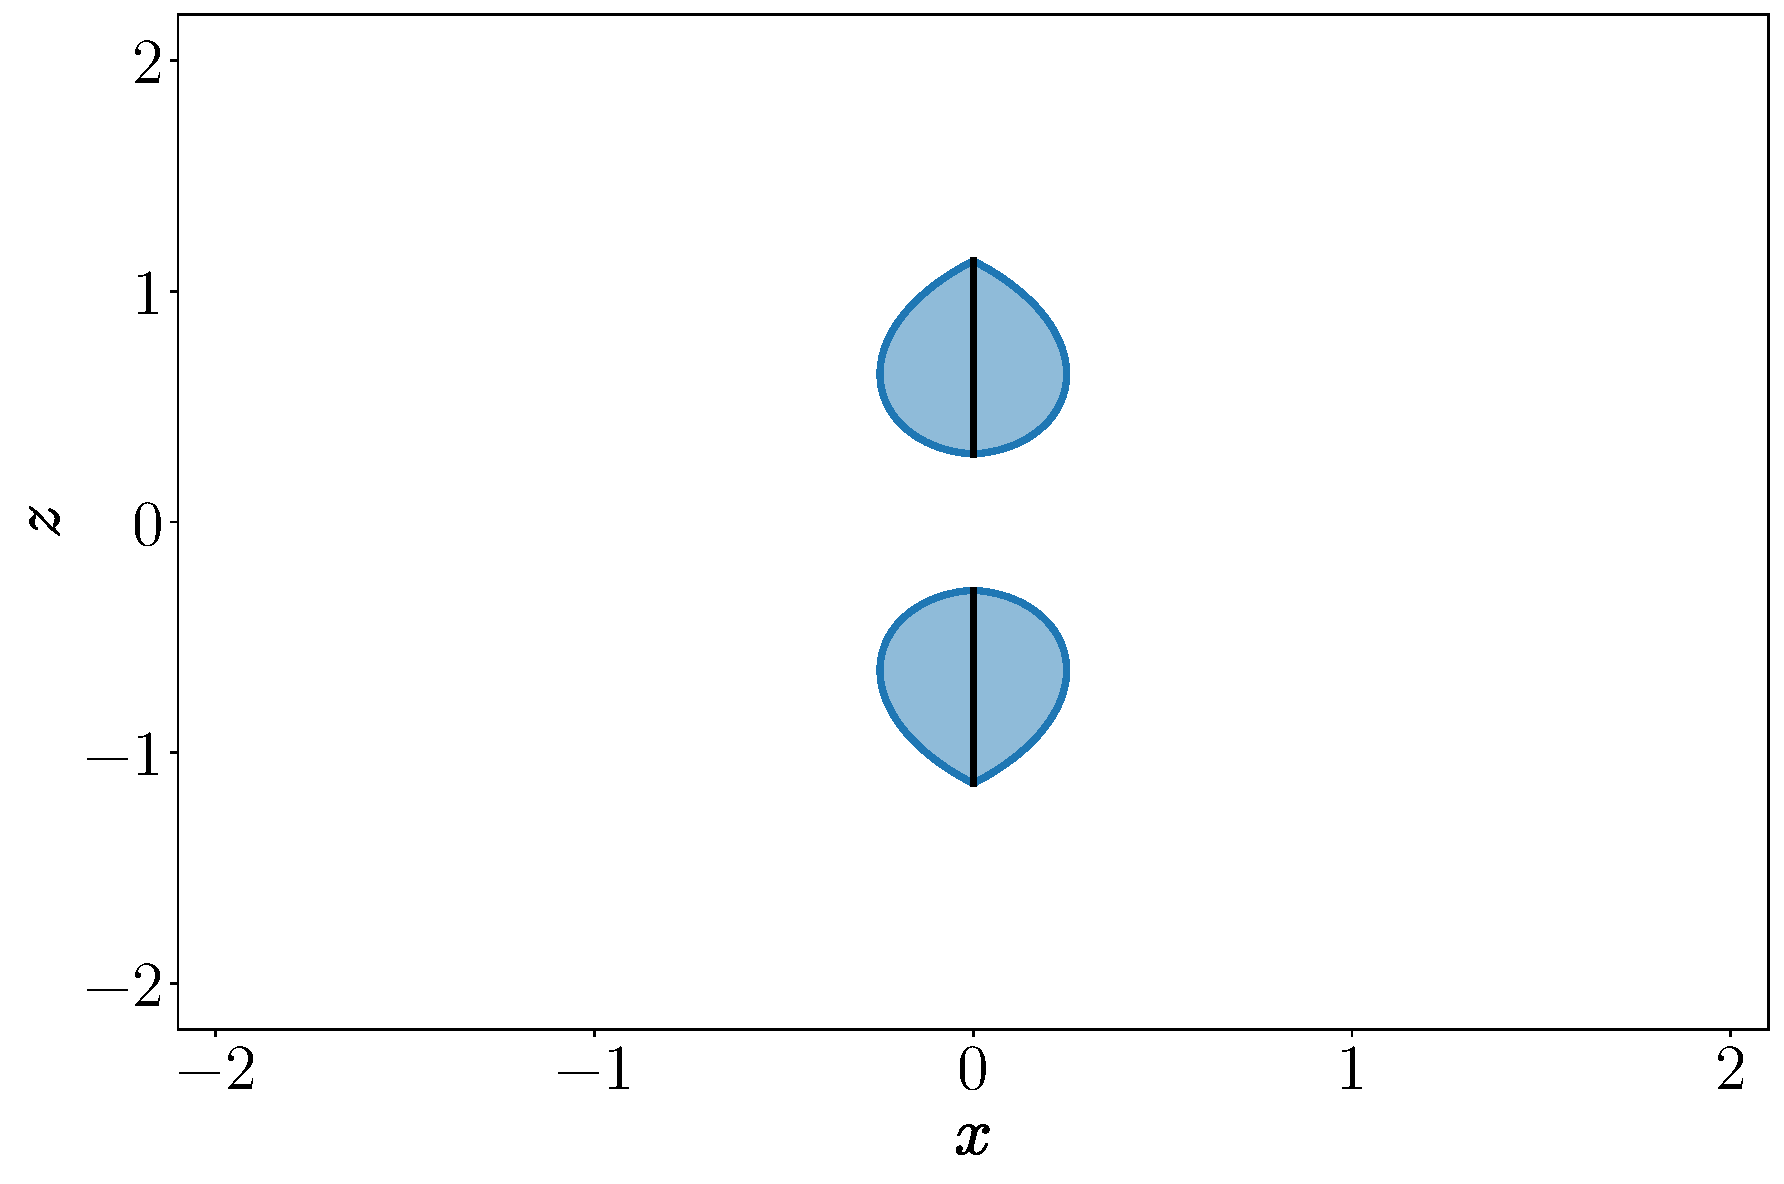
\includegraphics[scale = 0.22]{img/penrose_binaries/cmmr_ergo/ergo_b_0.7_q_1.0_a1_-0.65_a2_0.65.pdf}
    \label{ch:penrose_binaries/fig:ergo_unequal_c}
  }
  \subfloat[$b=0.98$]{
    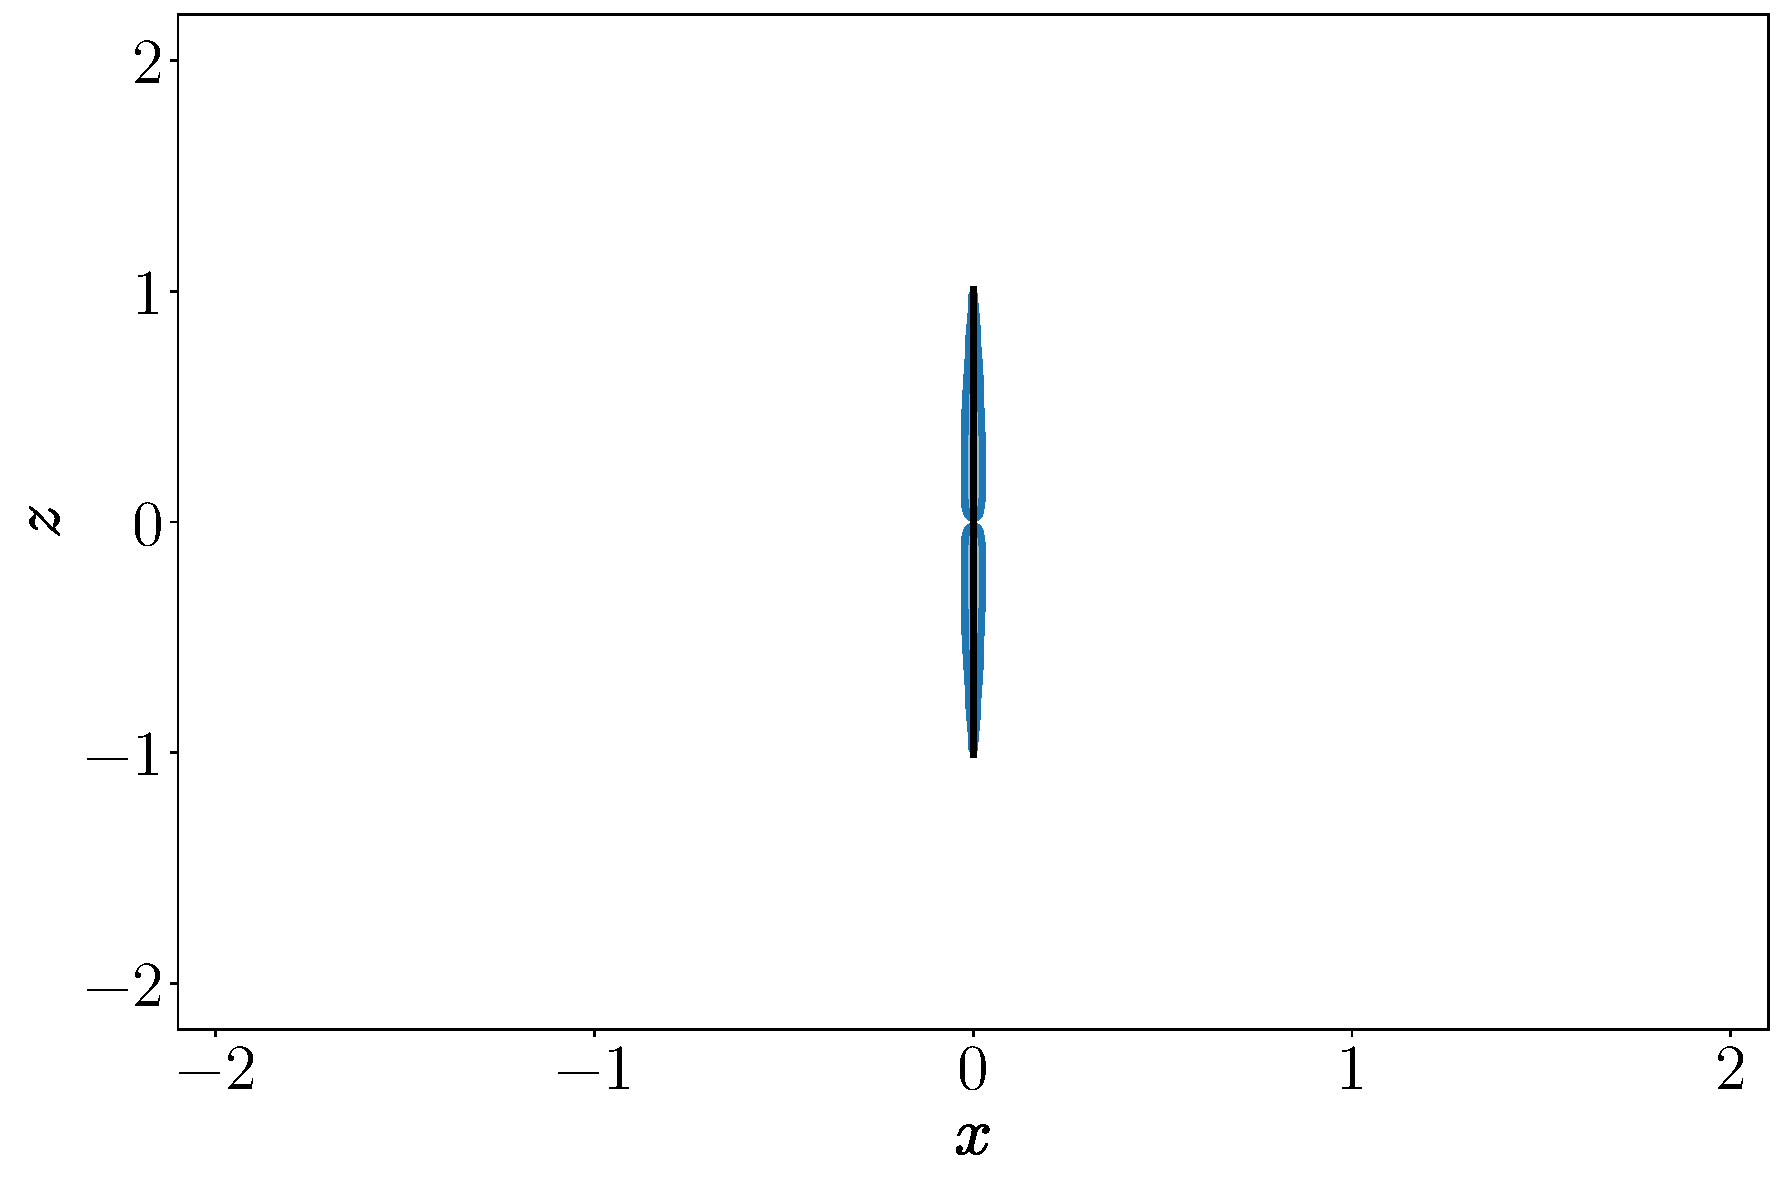
\includegraphics[scale = 0.22]{img/penrose_binaries/cmmr_ergo/ergo_b_0.98_q_1.0_a1_-0.65_a2_0.65}
    \label{ch:penrose_binaries/fig:ergo_unequal_d}
  }
  \caption{Ergosphere of a binary Kerr black hole system with mass ratio $q=1.0$ and aligned spins $a_1=0.65$ and $a_2=0.65$ for differente separation parameters. The blu region represents the ergosphere while the black lines represent the event horizons.}
  \label{ch:penrose_binaries/fig:ergo_unequal_spin}
\end{figure}

Let us now focus on Fig.~\ref{ch:penrose_binaries/fig:ergo_equal_spin}. As the holes get closer, the familiar ``infinity shaped'' ergosphere around each hole starts to deform in a very particular way: both of the tips of each ergosphere start to bend towards the other until they touch and eventually form a larger region that encompasses both holes and. Even more interesting, as the system gets closer to merging, the event horizons themselves get ``stretched'' along the $z$ direction. It becomes clear that in this case the ergospheres and event horizons ``add up'' to create structures larger than the originals.

Switching focus to Fig.~\ref{ch:penrose_binaries/fig:ergo_unequal_spin} that in spite of the fact that the event horizons still ``stretch'' what appears to be the opposite of the aligned spin case happens for the ergospheres. Instead of bending towards each other they are repelled to the point that when they are close to merging, their shape becomes very thin and elongated. In other words, the ergospheres become \textit{spaghettifyied} and ``cancel out'' in the case of equal but anti-aligned spins.

These results are not physically surprising. One expects that black holes that have exactly the same spin but in opposite directions when merged create a resulting black hole that has more mass but no spin, that is, their counter rotation balances and cancels out. The opposite is expected to happen for black holes with aligned spins: both their masses and angular momenta are added up upon merging. The novelty of our work is, we believe, in the fact that even using an analytic solution containing an unphysical strut that keeps the black holes from colliding such features are apparent and can be demonstrated with relative ease.

Now that the general shapes and features of the ergospheres have been established, we can ask ourselves how far appart should the Kerr black holes be so that their individual ergospheres merge into one? From Fig.~\ref{ch:penrose_binaries/fig:ergo_unequal_spin} we can see that if the spins are exactly equal in modulus but differ in sign such merging is impossible. Nevertheless, from Fig.~\ref{ch:penrose_binaries/fig:ergo_equal_spin} we see that when the spins are equal we can be sure that such merging occurs for some value of $b$. It is not unreasonable to imagine that in the intermediary case is considered, that is anti-aligned spins that are not exactly equal, such merging also occurs.

In order to visualize the parameter regions that are able to produce connected ergospheres we plot the regions for which the parameters produce physical black hole binarys (i.e., black holes and not naked singularities) and $f(\rho,0) = 0$ for some value of $\rho$. These are the blue regions shown in Fig.~\ref{ch:penrose_binaries/fig:ergo_joined} where we increased $b$ from $0.89$ to $0.98$ while also increasing the mass ratio from $0.1$ to $1.0$ and in Fig.~\ref{ch:penrose_binaries/fig:ergo_joined_2} where $a_1$ and $q$ where fixed but $a_2$ and $b$ were allowed to change instead. It is extremely important to point out that despite what the figures indicate the configuration $a_1=a_2=0$ does not produce an ergosphere. These points are included in our graphs but should be disregarded as the CMMR solution in the form presented in Ref.~\cite{MANKO2020} (which is the source of all metric quantities used in this work) does not describe the black hole system correctly if one of the spins is zero. This case must be treated separately and is discussed in detail in Ref.~\cite{MANKO2019}.

Let us now focus on Fig.~\ref{ch:penrose_binaries/fig:ergo_joined}. For any given mass ratio, it is apparent that the increase in the distance parameter increases the overall size of the parameter region producing joint ergospheres. The most interesting feature is that certain configurations of equal but opposite spins can also produce a joined ergosphere if the masses are not equal. This can be easily seen in Fig.~\ref{ch:penrose_binaries/fig:ergo_joined_e} if $a_1=0.5$ and $a_2=-0.5$.

In Fig.~\ref{ch:penrose_binaries/fig:ergo_joined_2} we look at the influence of the distance parameter in more detail. The first apparent feature is that for equal mass binaries, the configuration where $a_2=-a_1$ never produces a joined ergosphere, even for very large distance parameters (and thus very small distances). This can easily be seen in Fig.~\ref{ch:penrose_binaries/fig:ergo_joined_2_b} and Fig.~\ref{ch:penrose_binaries/fig:ergo_joined_2_d}. We can also observe that for a fixed mas ratio, an increase in the fixed spin parameter $a_1$ causes the area of the graph to become larger in the negative region of $a_2$ which can be seen in Fig.~\ref{ch:penrose_binaries/fig:ergo_joined_2_a} and Fig.~\ref{ch:penrose_binaries/fig:ergo_joined_2_c}. This indicates that for binaries with unequal masses, configurations with opposite spins can generate joined ergospheres more easily. Furthermore we can observe the universal need of $b$ being large in order to create joined ergospheres.

\begin{figure}
  \centering
  \subfloat[$b=0.89$, $q=0.1$]{
    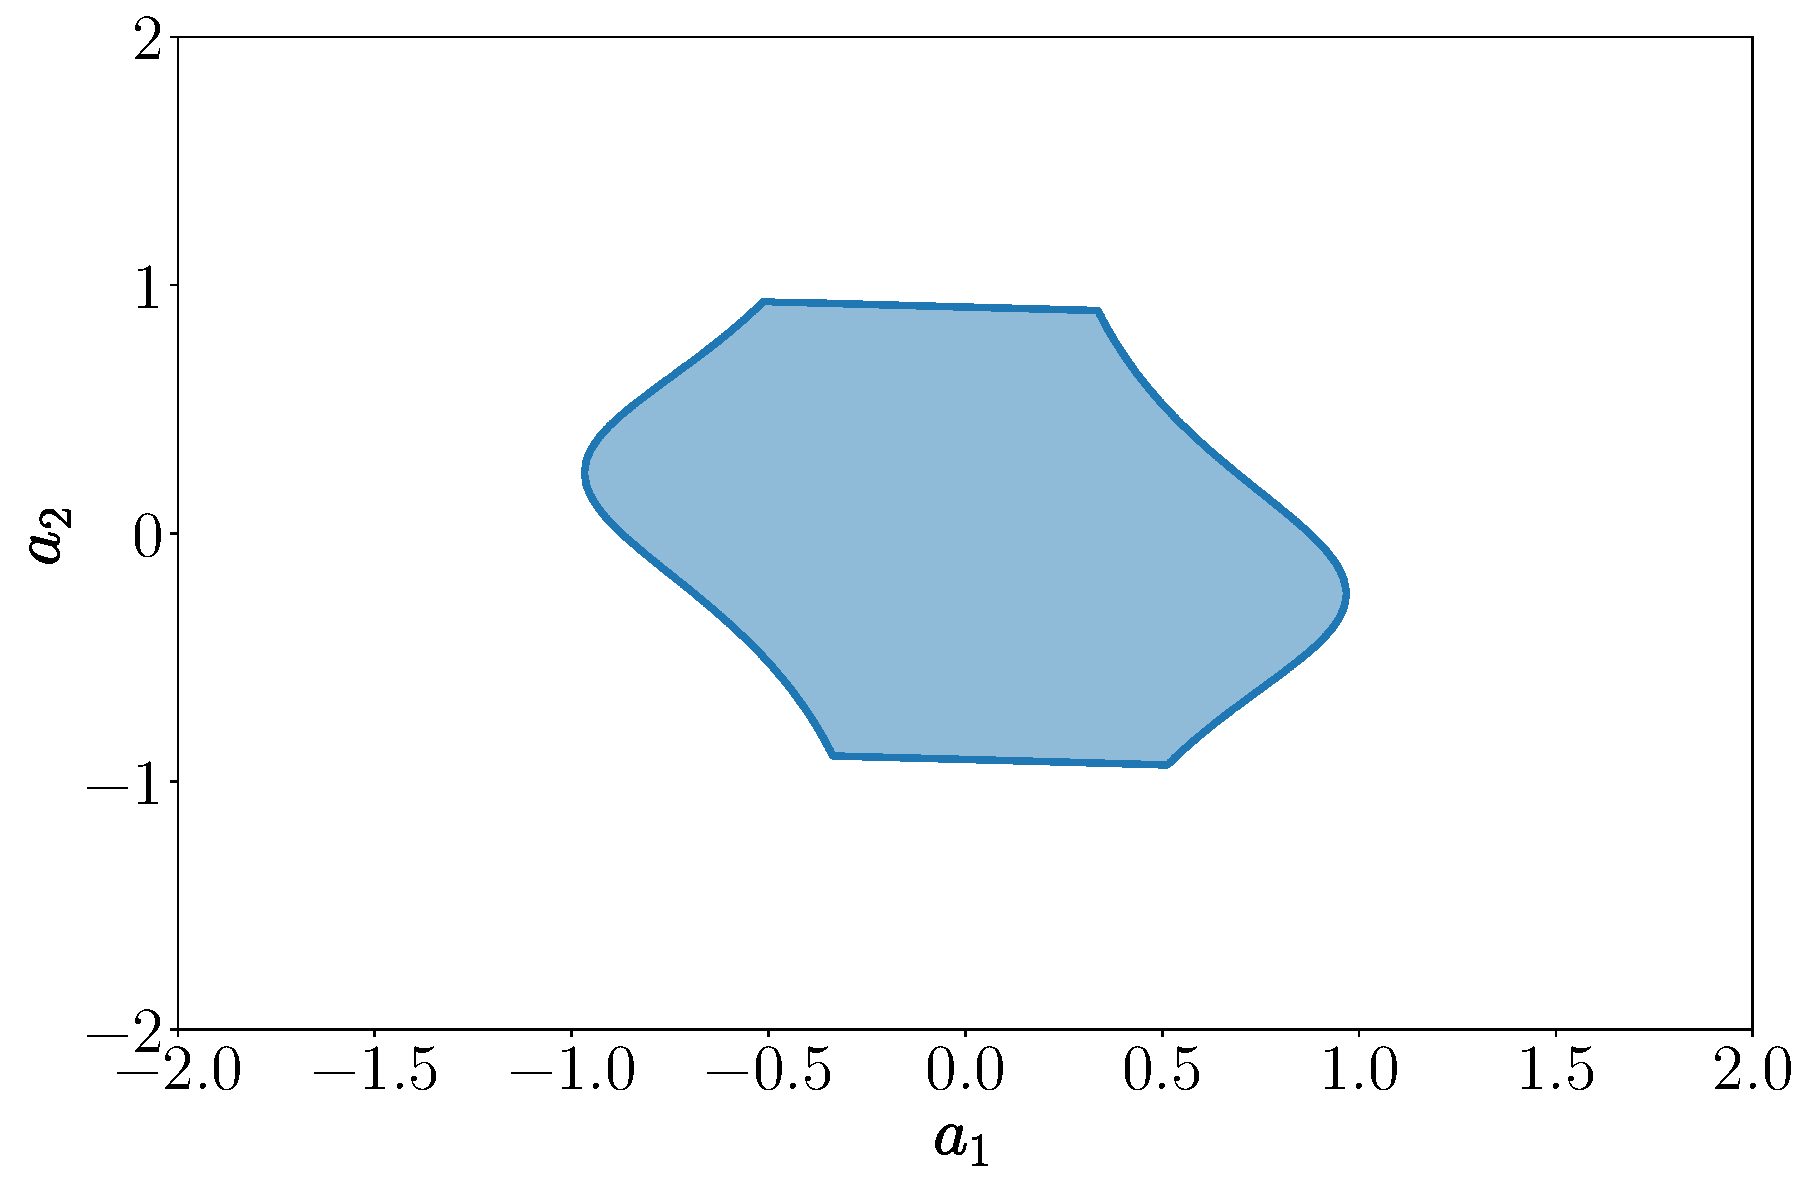
\includegraphics[scale = 0.15]{img/penrose_binaries/cmmr_joined_ergo/joined_ergo_b_0.89_q_0.1}
    \label{ch:penrose_binaries/fig:ergo_joined_a}
  }
  \subfloat[$b=0.89$, $q=0.5$]{
    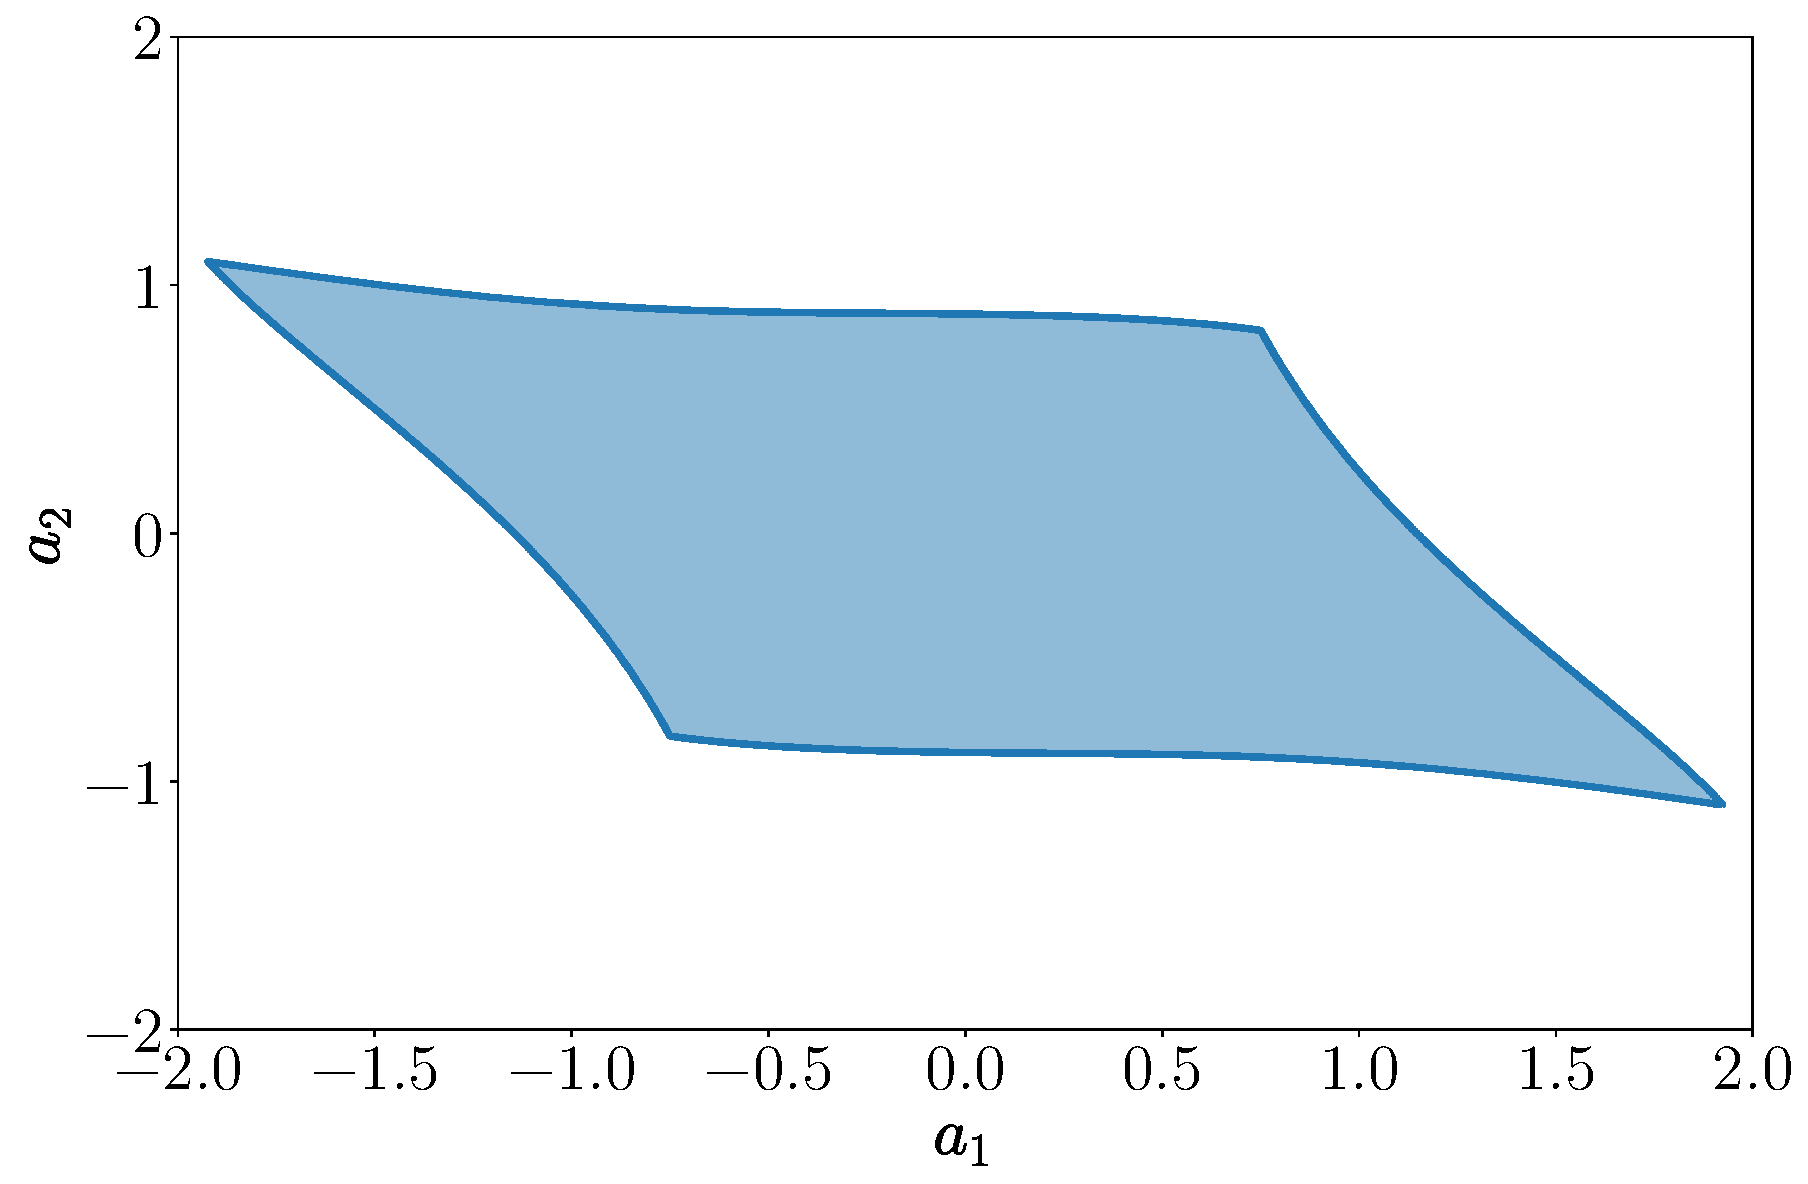
\includegraphics[scale = 0.15]{img/penrose_binaries/cmmr_joined_ergo/joined_ergo_b_0.89_q_0.5}
    \label{ch:penrose_binaries/fig:ergo_joined_b}
  }
  \subfloat[$b=0.89$, $q=1.0$]{
    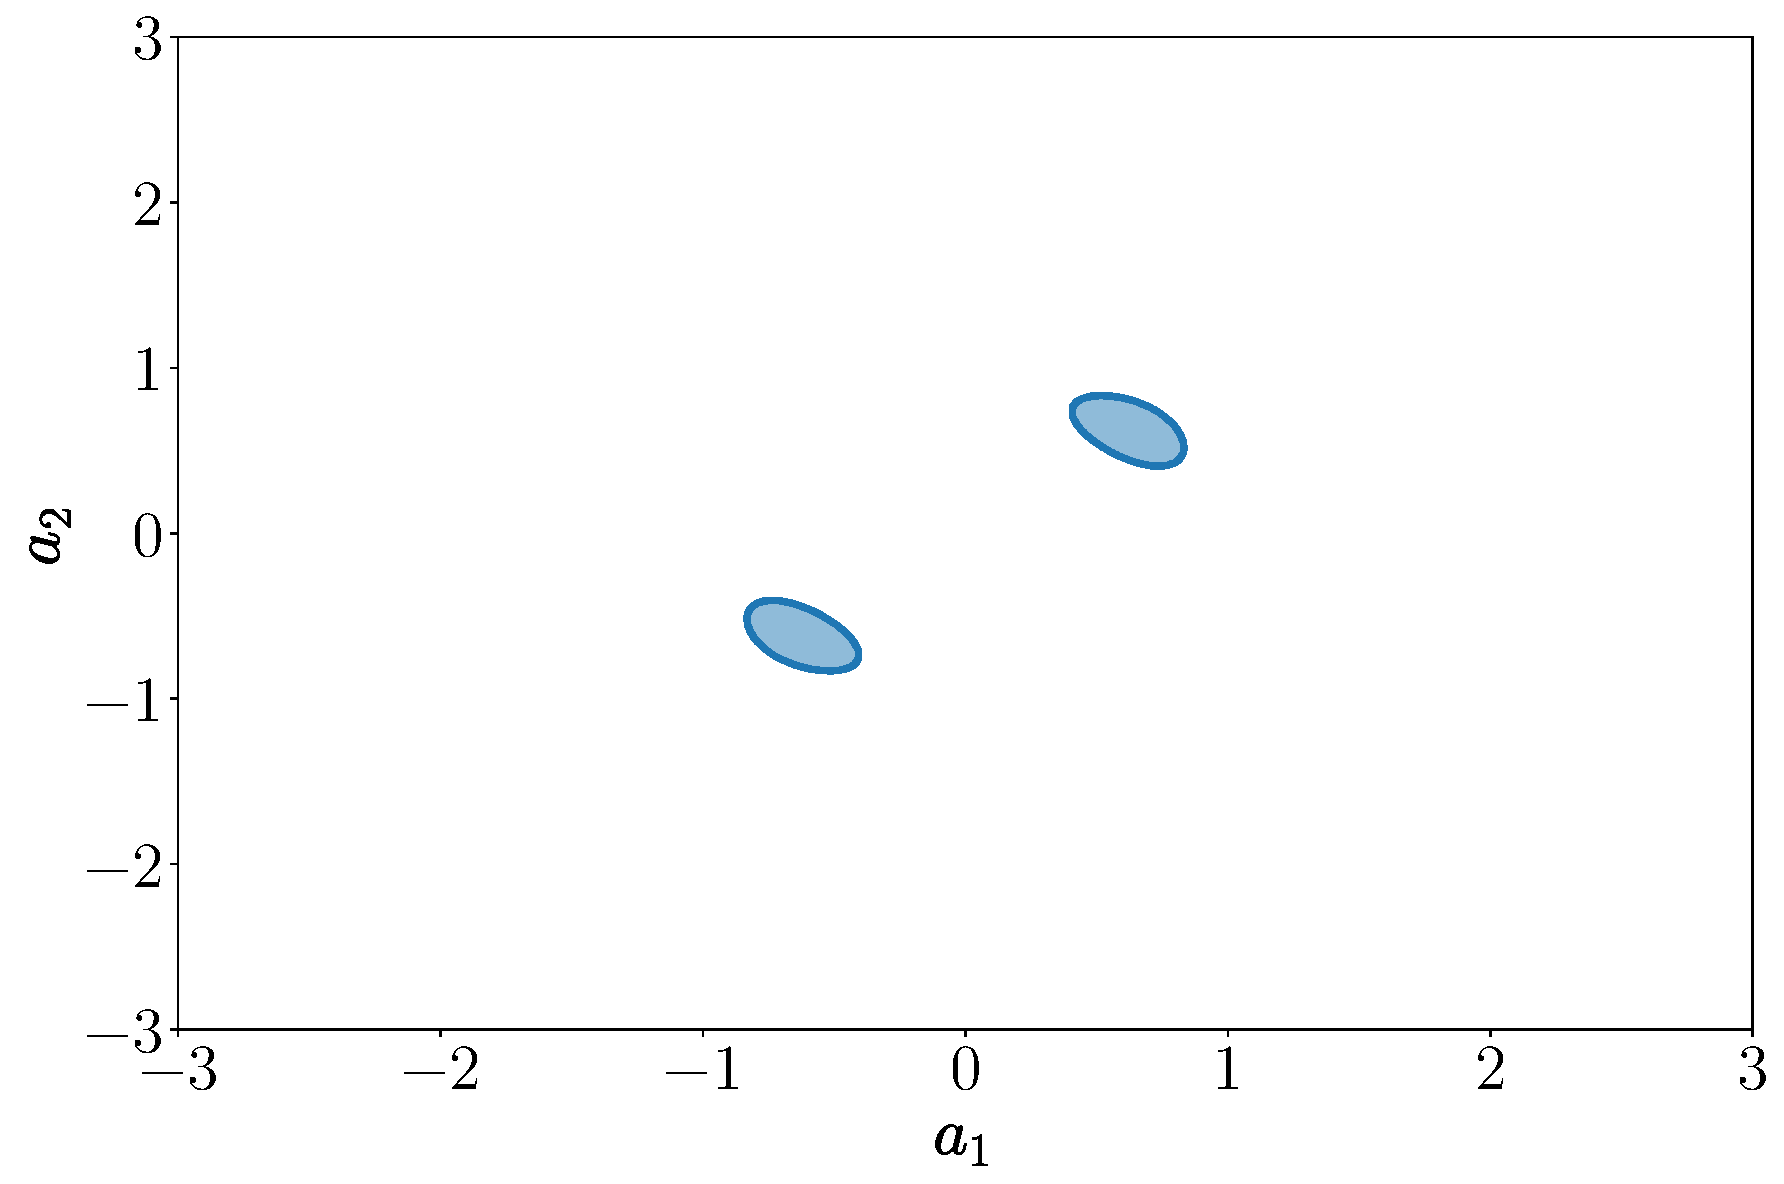
\includegraphics[scale = 0.15]{img/penrose_binaries/cmmr_joined_ergo/joined_ergo_b_0.89_q_1.0}
    \label{ch:penrose_binaries/fig:ergo_joined_c}
  }
  \newline
  \subfloat[$b=0.93$, $q=0.1$]{
    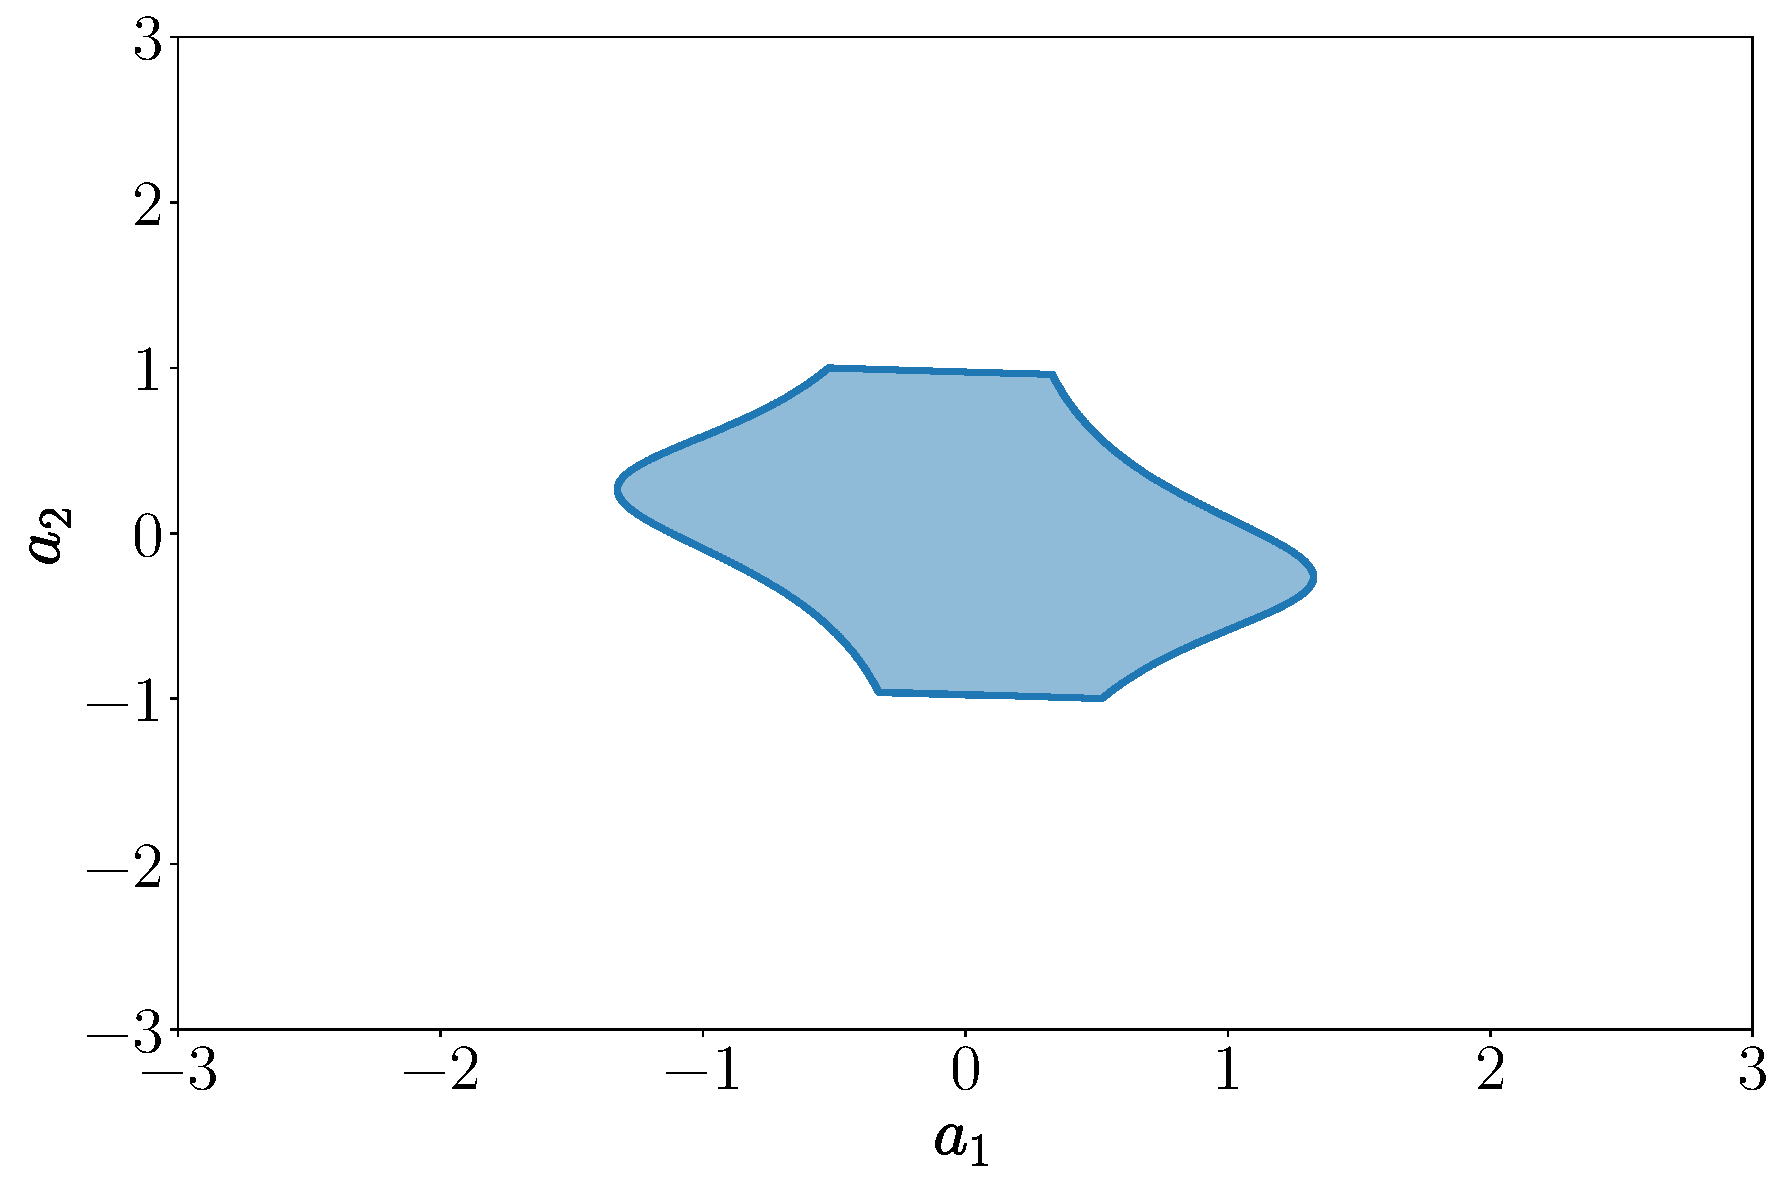
\includegraphics[scale = 0.15]{img/penrose_binaries/cmmr_joined_ergo/joined_ergo_b_0.93_q_0.1}
    \label{ch:penrose_binaries/fig:ergo_joined_d}
  }
  \subfloat[$b=0.93$, $q=0.5$]{
    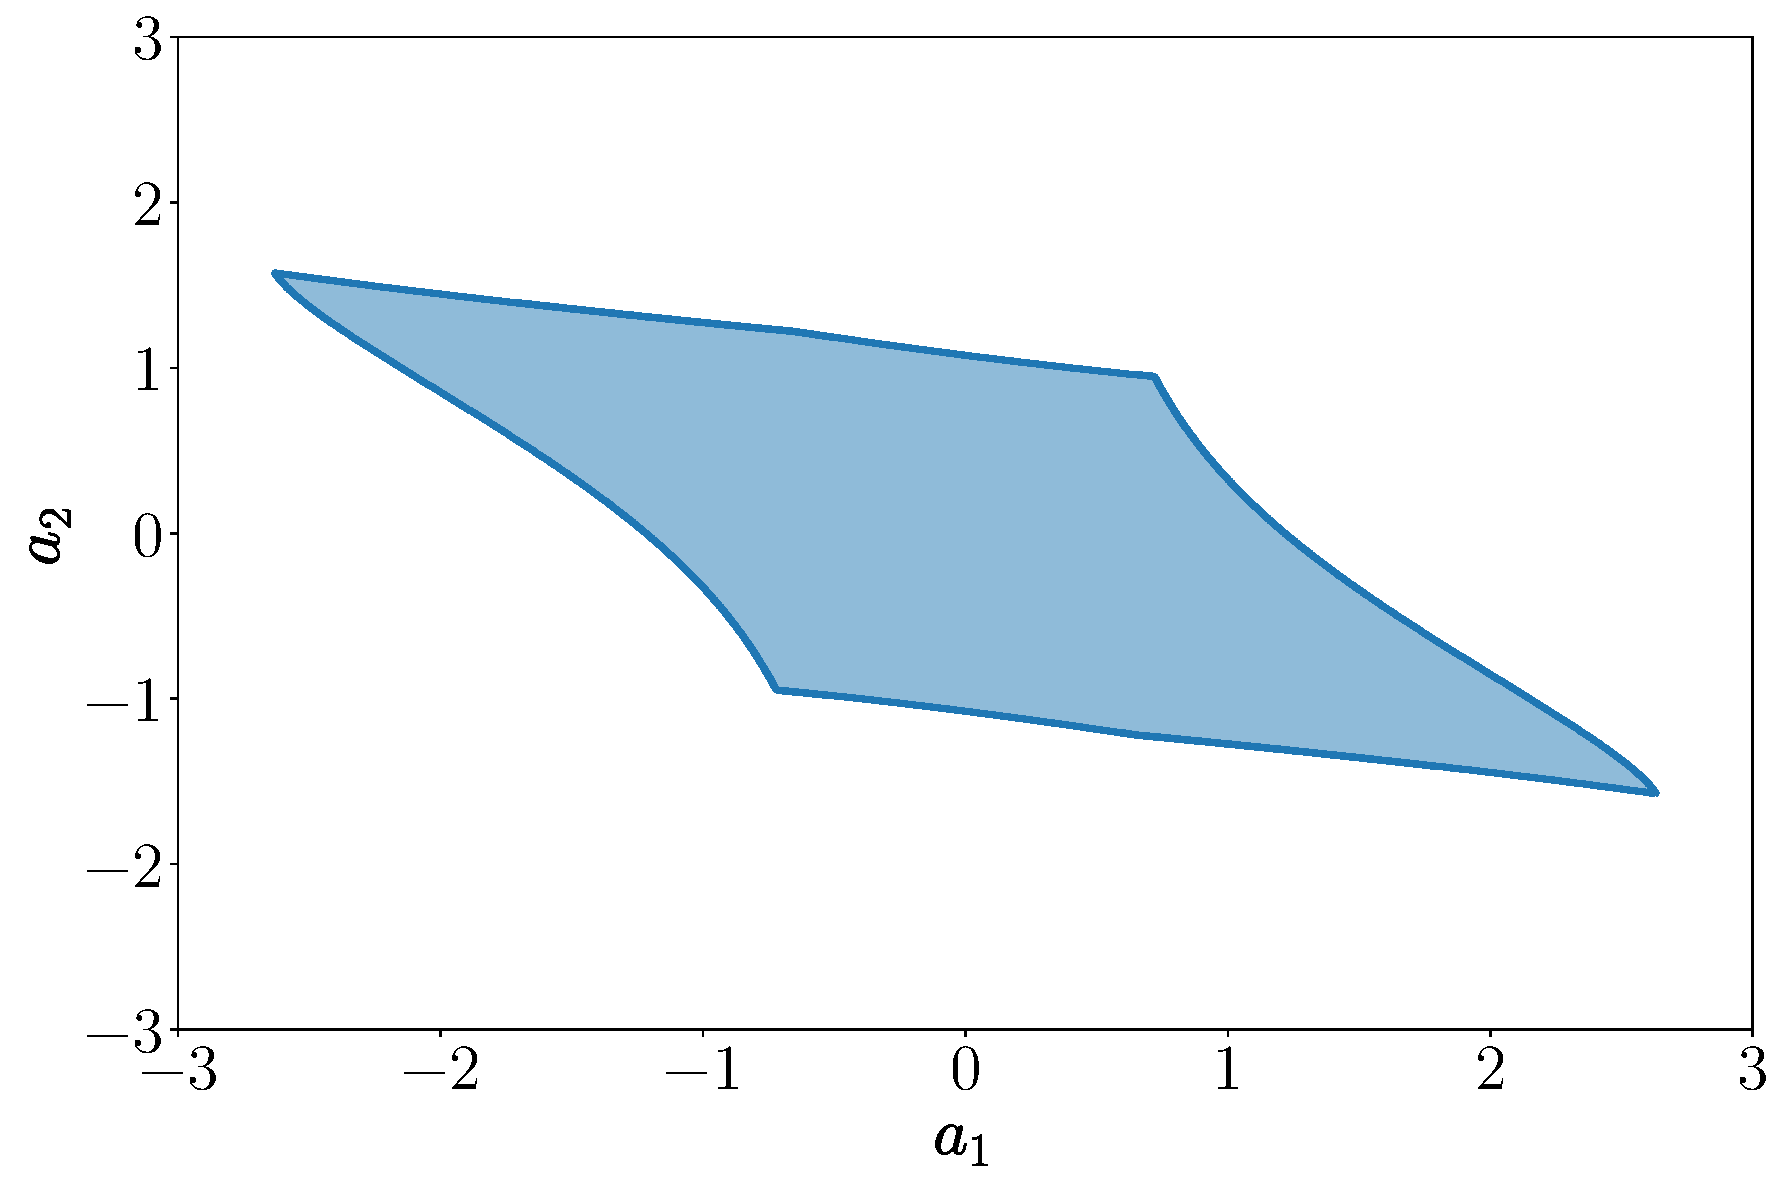
\includegraphics[scale = 0.15]{img/penrose_binaries/cmmr_joined_ergo/joined_ergo_b_0.93_q_0.5}
    \label{ch:penrose_binaries/fig:ergo_joined_e}
  }
  \subfloat[$b=0.93$, $q=1.0$]{
    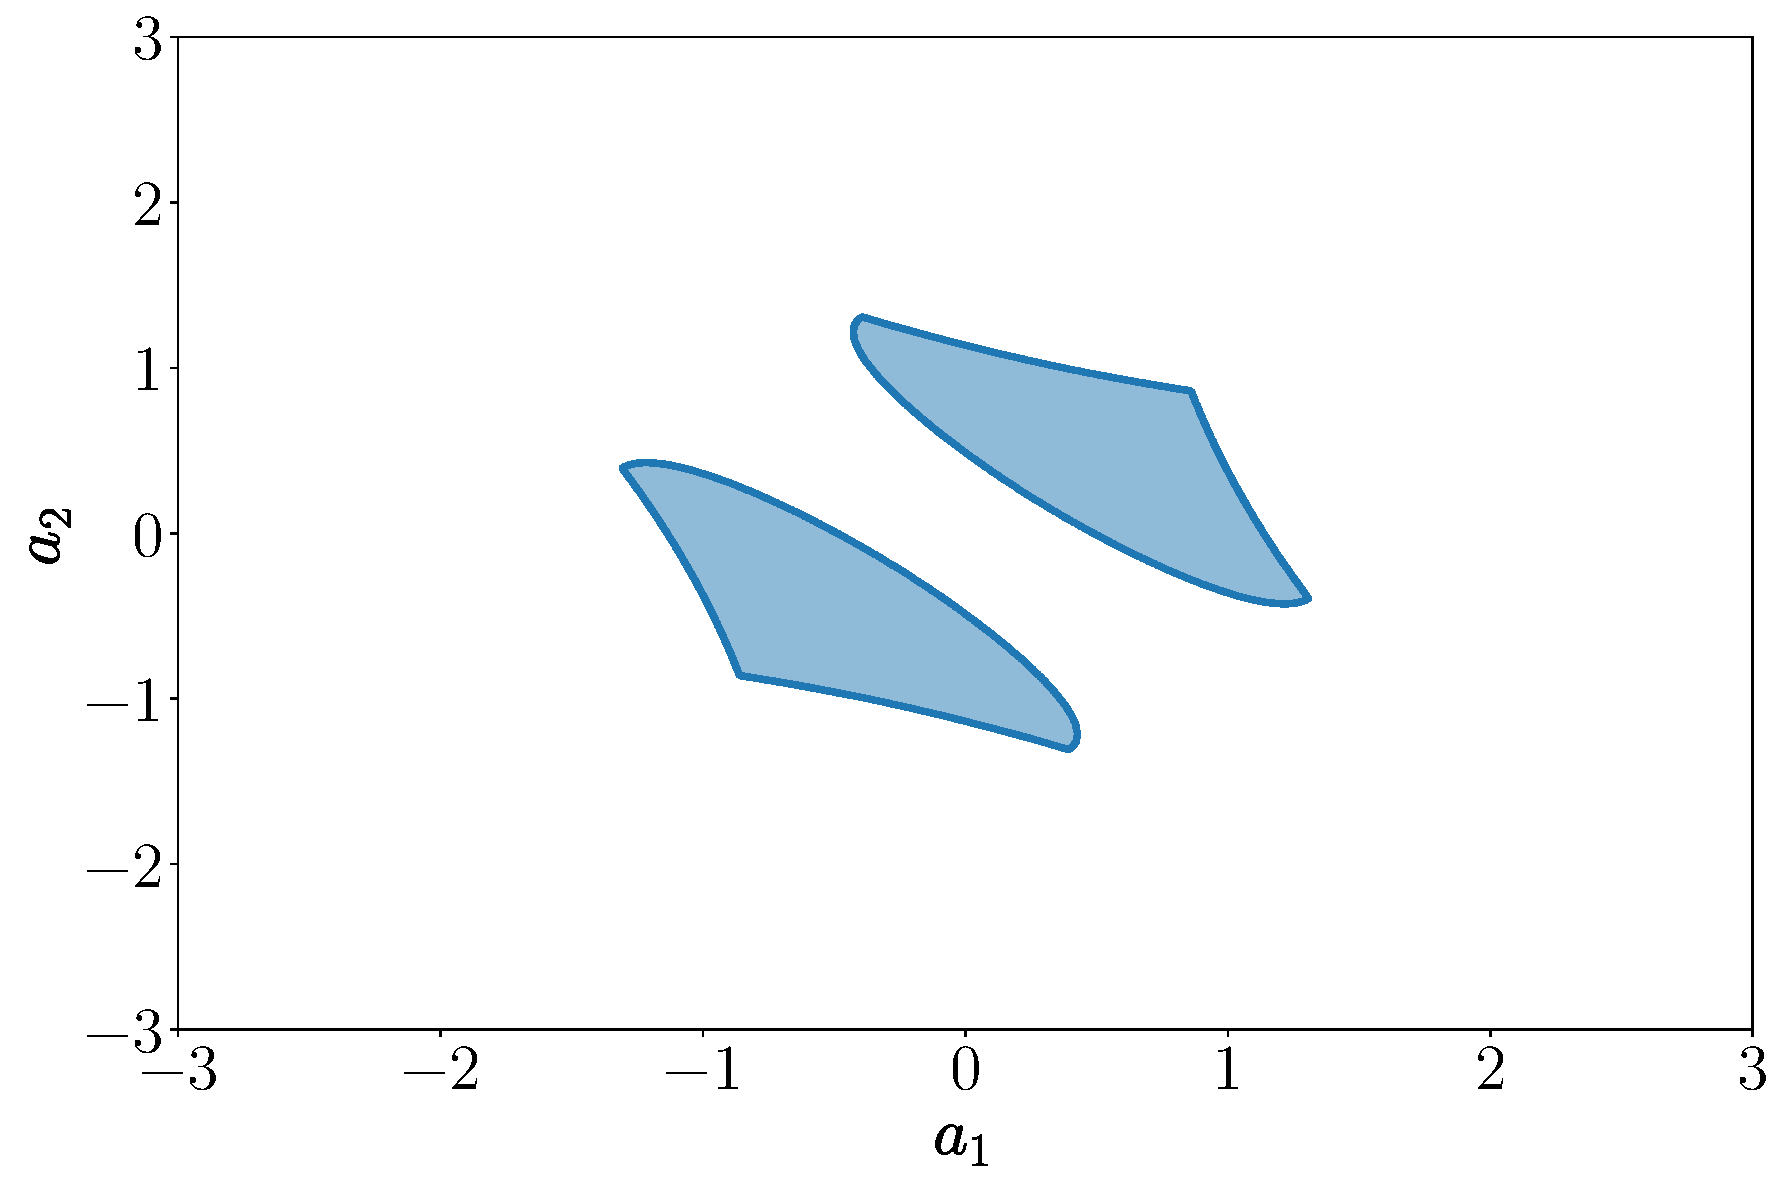
\includegraphics[scale = 0.15]{img/penrose_binaries/cmmr_joined_ergo/joined_ergo_b_0.93_q_1.0}
    \label{ch:penrose_binaries/fig:ergo_joined_f}
  }
  \newline
  \subfloat[$b=0.98$, $q=0.1$]{
    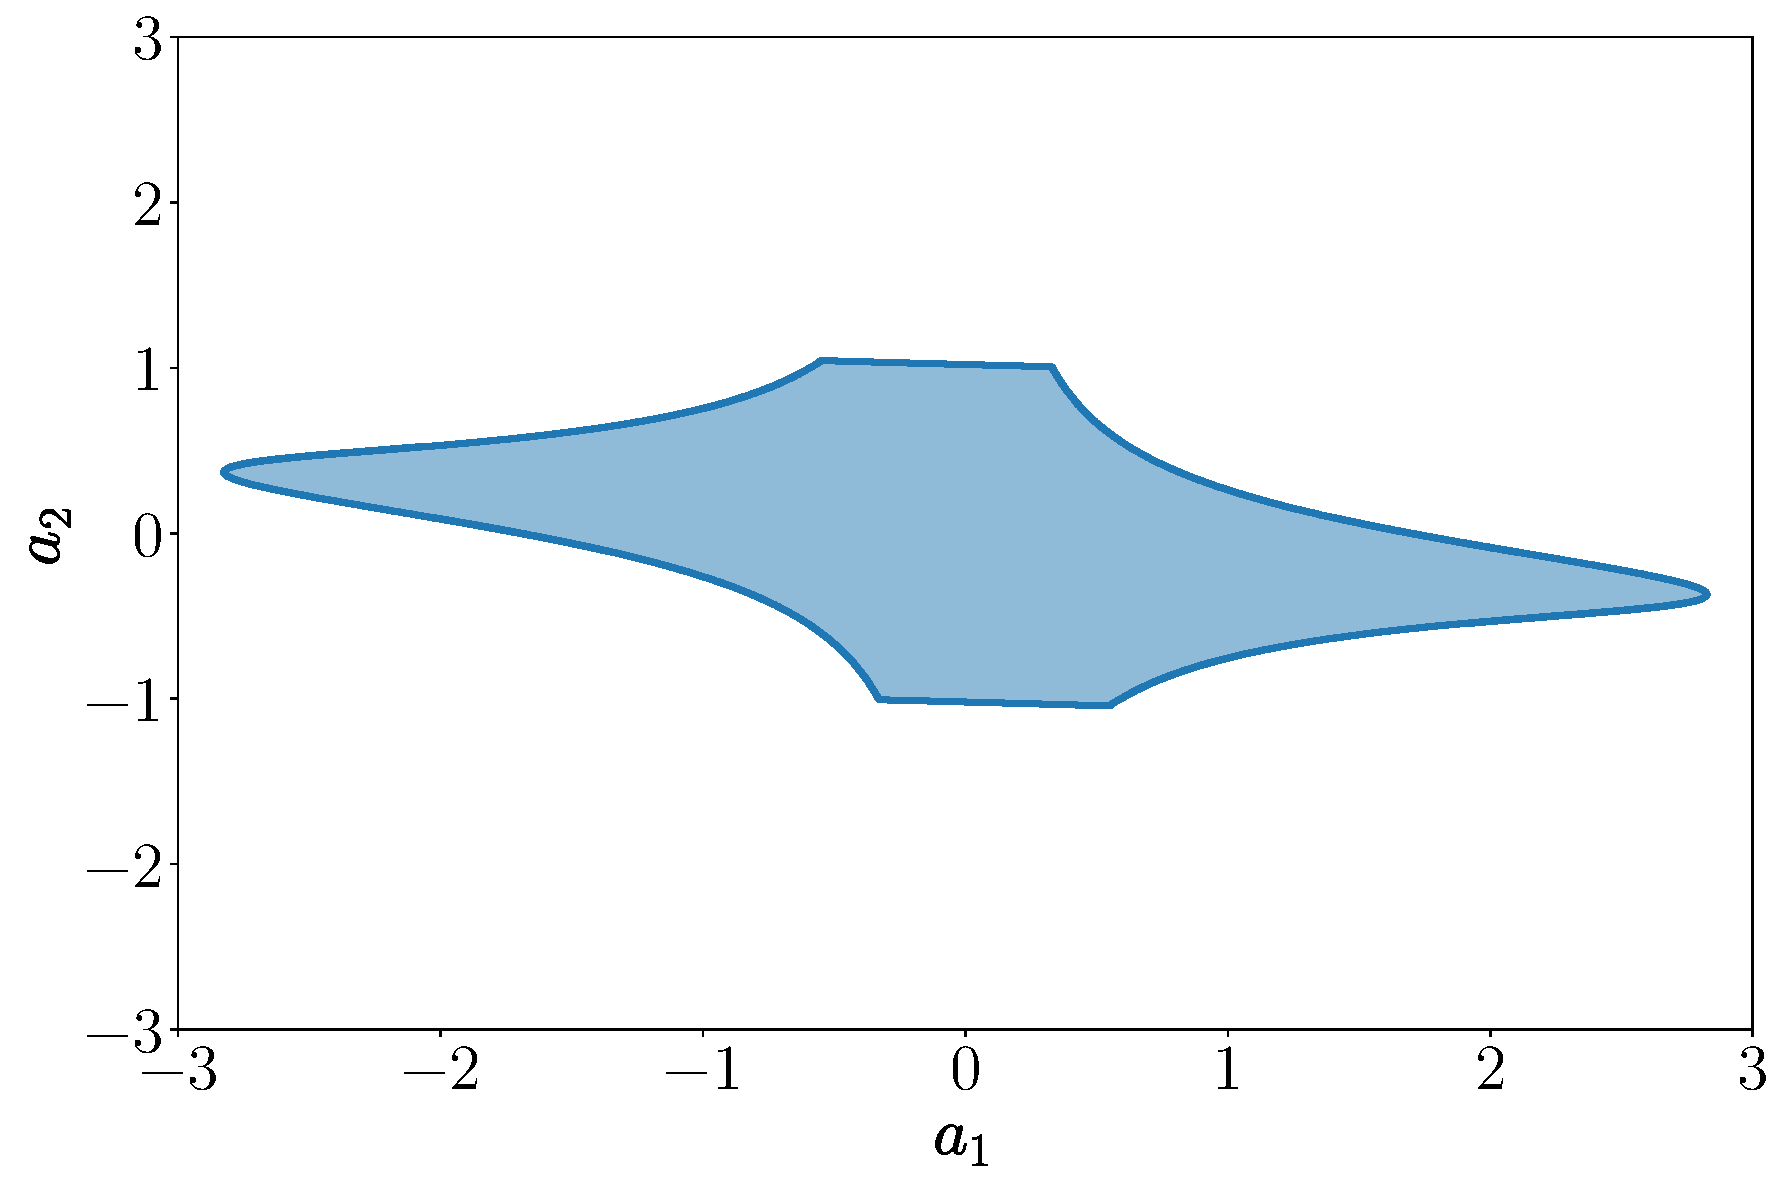
\includegraphics[scale = 0.15]{img/penrose_binaries/cmmr_joined_ergo/joined_ergo_b_0.98_q_0.1}
    \label{ch:penrose_binaries/fig:ergo_joined_g}
  }
  \subfloat[$b=0.98$, $q=0.5$]{
    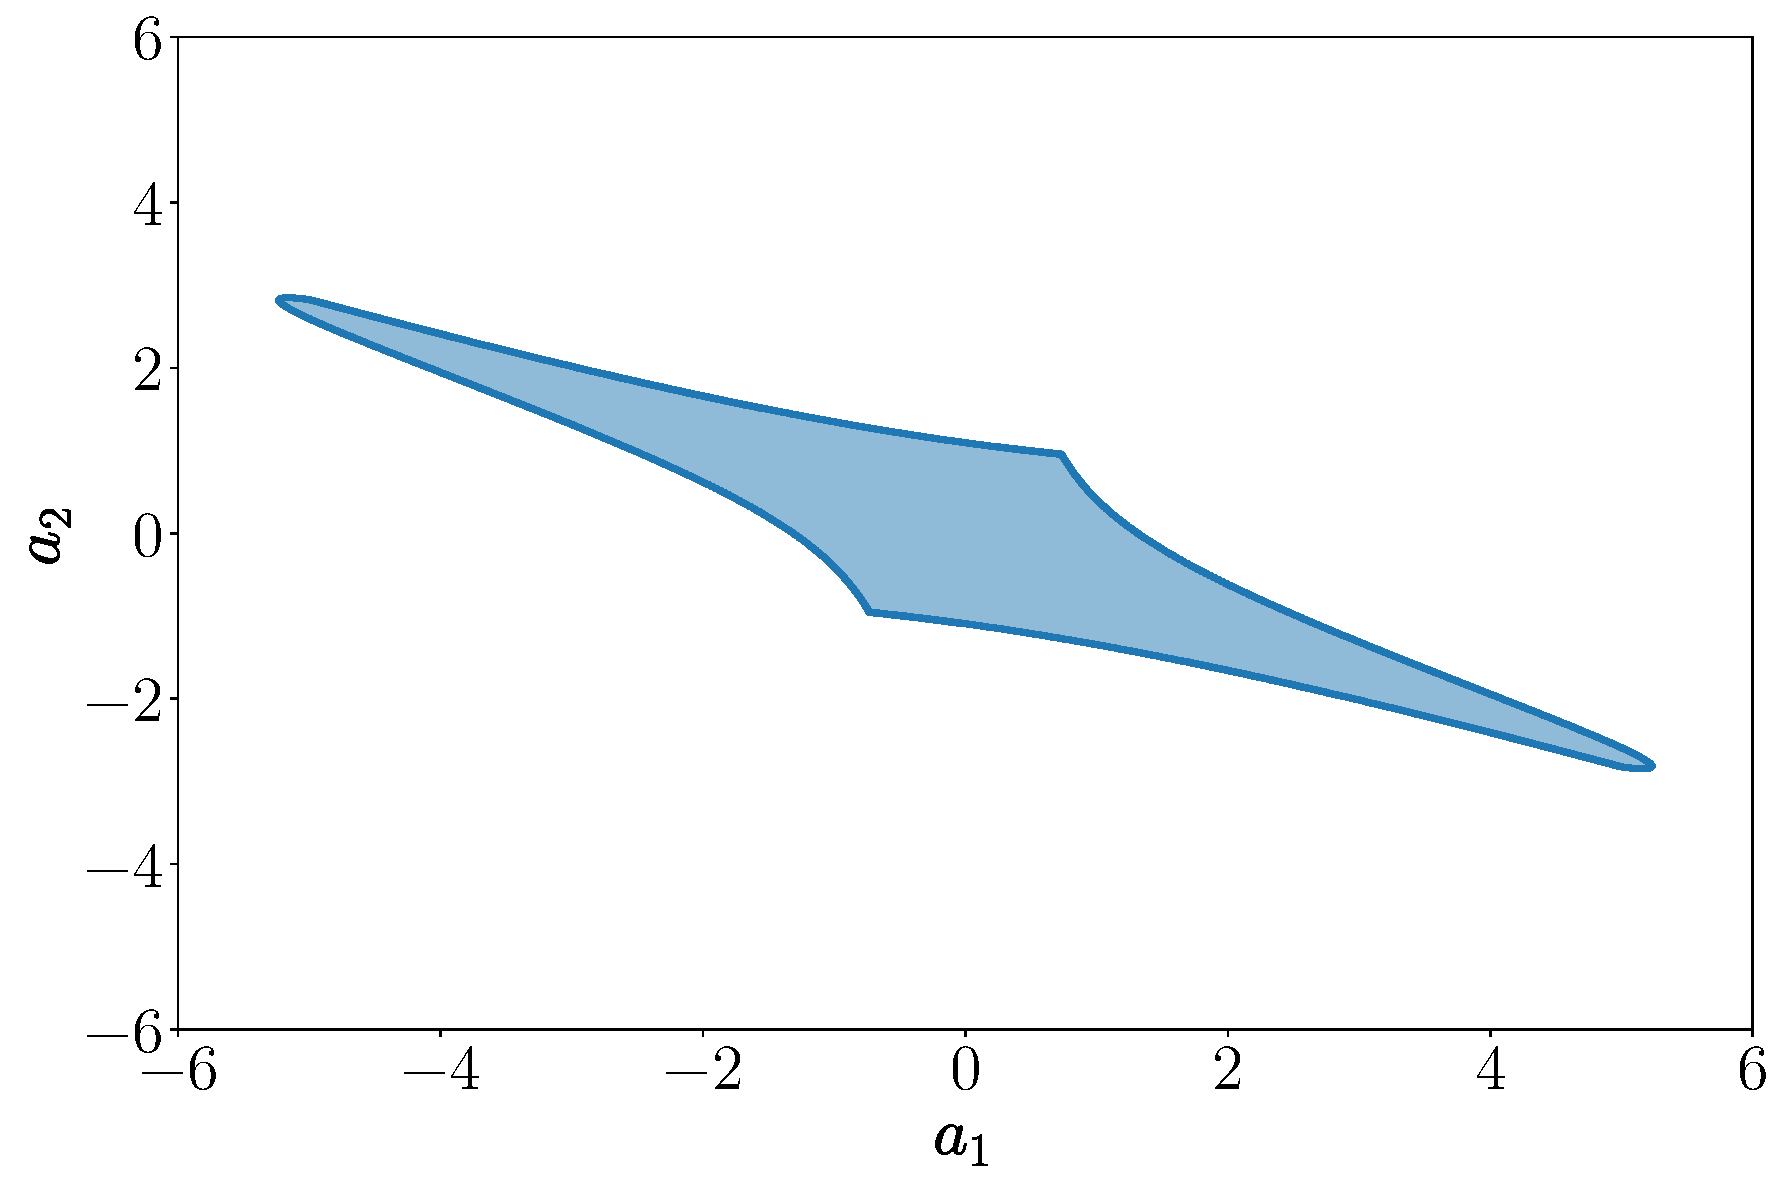
\includegraphics[scale = 0.15]{img/penrose_binaries/cmmr_joined_ergo/joined_ergo_b_0.98_q_0.5}
    \label{ch:penrose_binaries/fig:ergo_joined_h}
  }
  \subfloat[$b=0.98$, $q=1.0$]{
    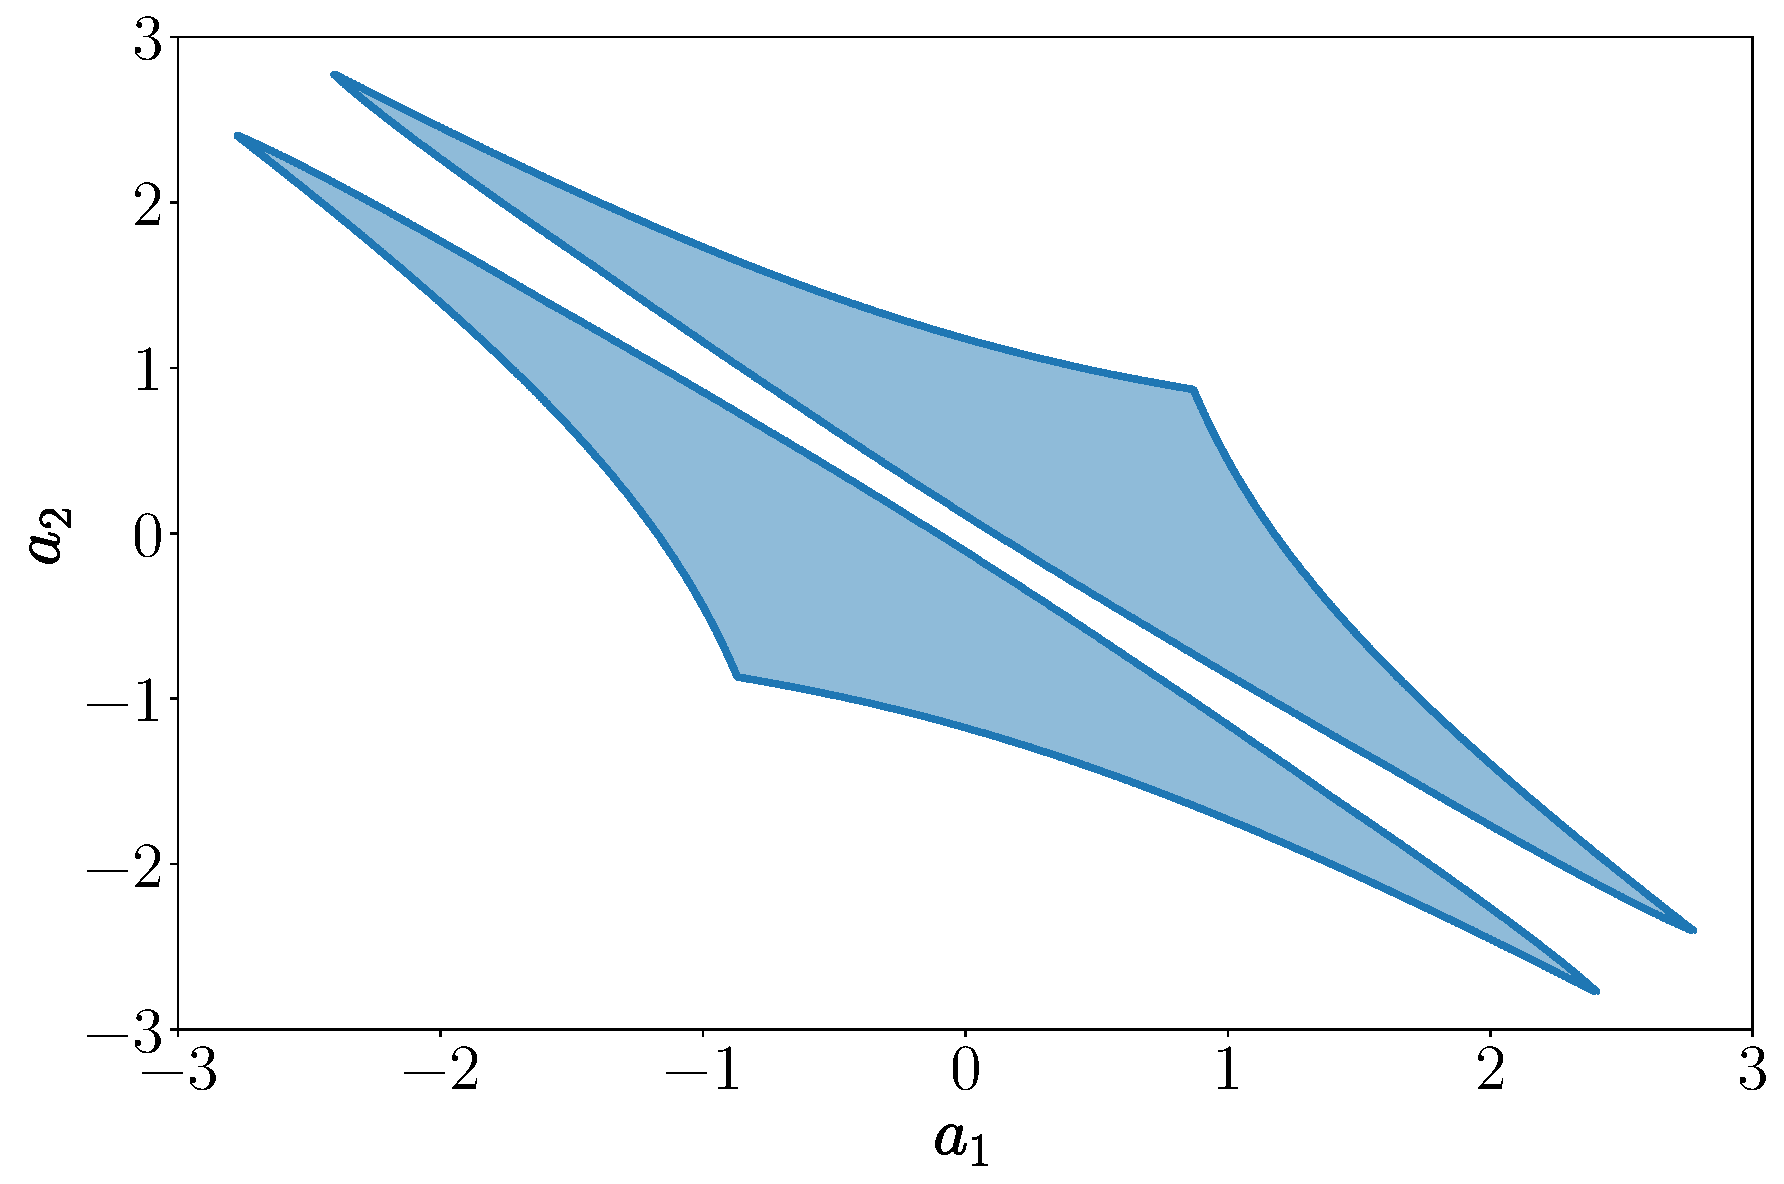
\includegraphics[scale = 0.15]{img/penrose_binaries/cmmr_joined_ergo/joined_ergo_b_0.98_q_1.0}
    \label{ch:penrose_binaries/fig:ergo_joined_i}
  }
  \caption{Parameter spaces that allow for a common ergosphere. The blue regions represent pairs of $a_1$ and $a_2$ values that produce an ergosphere around both black holes for each $(b,q)$  indicated value.}
  \label{ch:penrose_binaries/fig:ergo_joined}
\end{figure}

\begin{figure}
  \centering
  \subfloat[$a_1=1.0$, $q=0.5$]{
    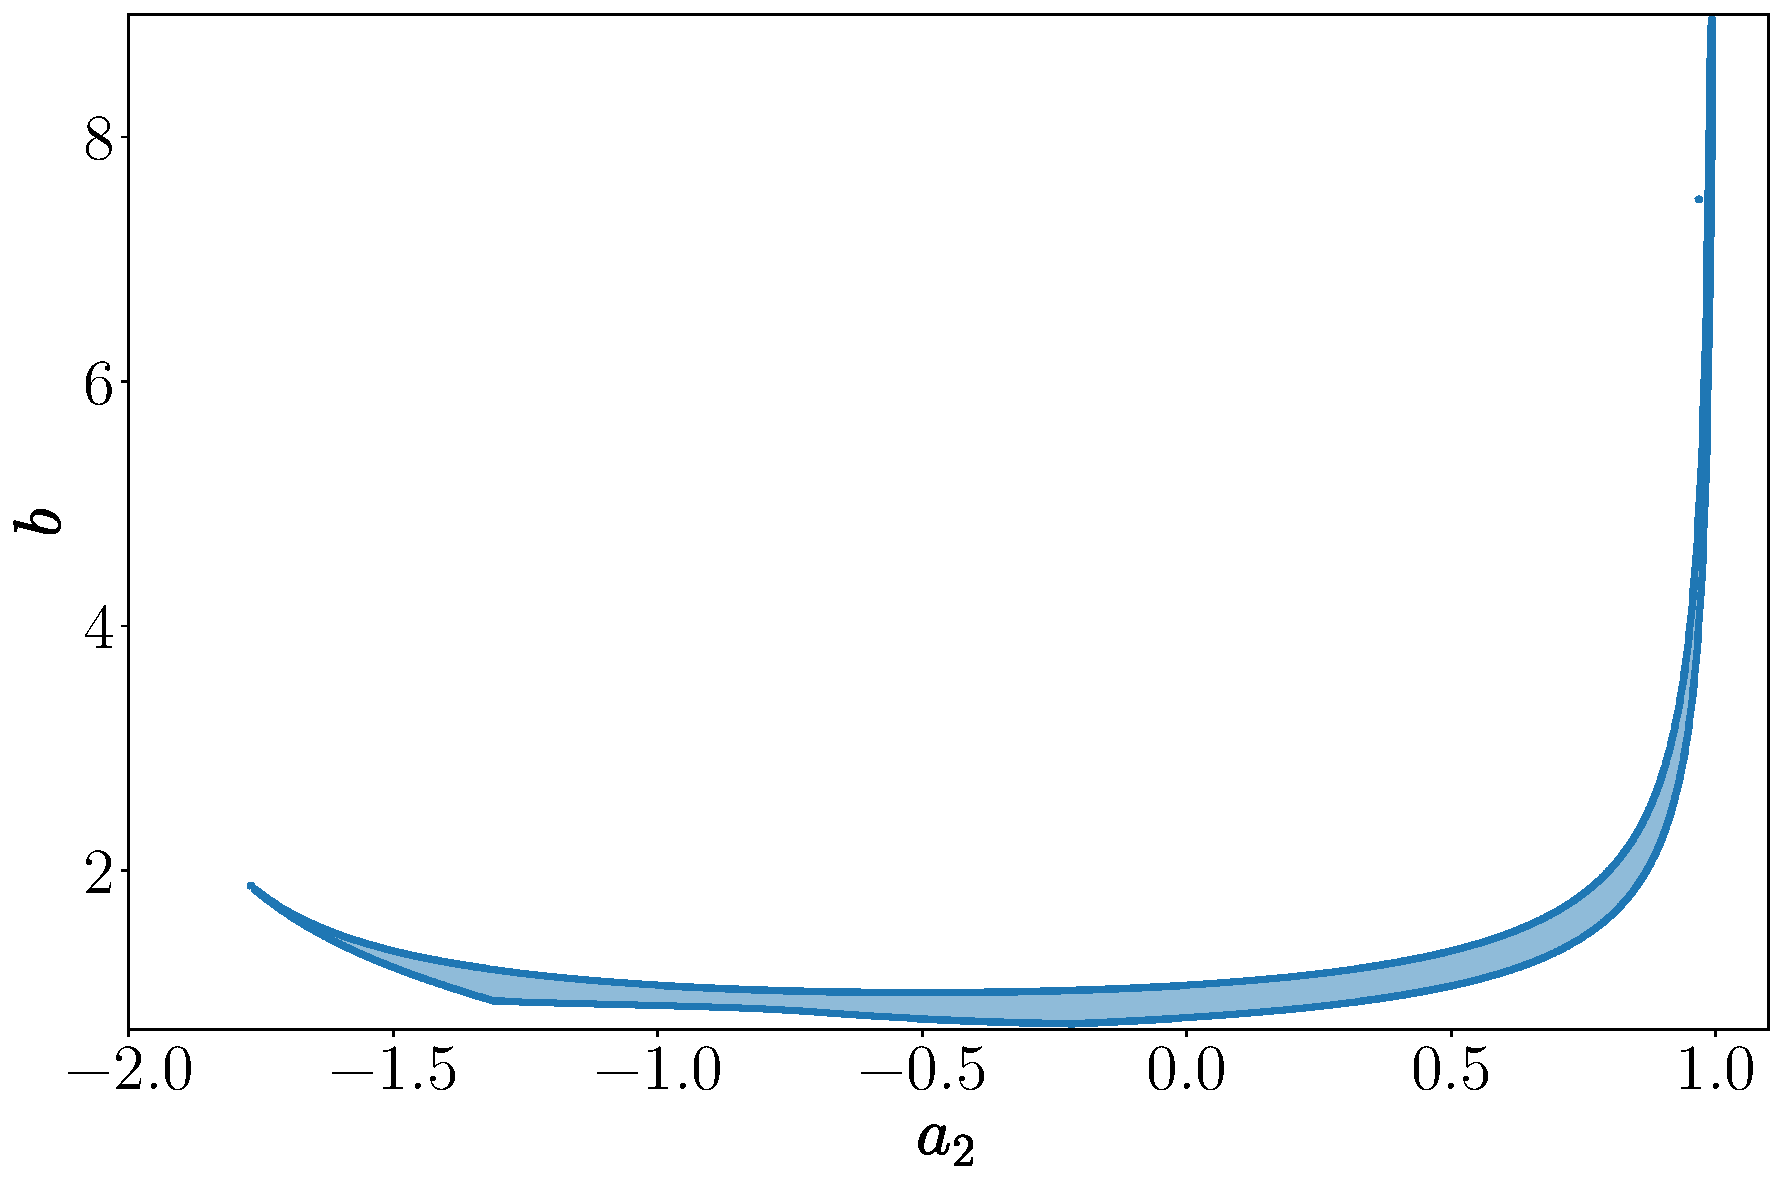
\includegraphics[scale = 0.22]{img/penrose_binaries/cmmr_joined_ergo/joined_ergo_2_a1_1.0_q_0.5.pdf}
    \label{ch:penrose_binaries/fig:ergo_joined_2_a}
  }
  \subfloat[$a_1=1.0$, $q=1.0$]{
    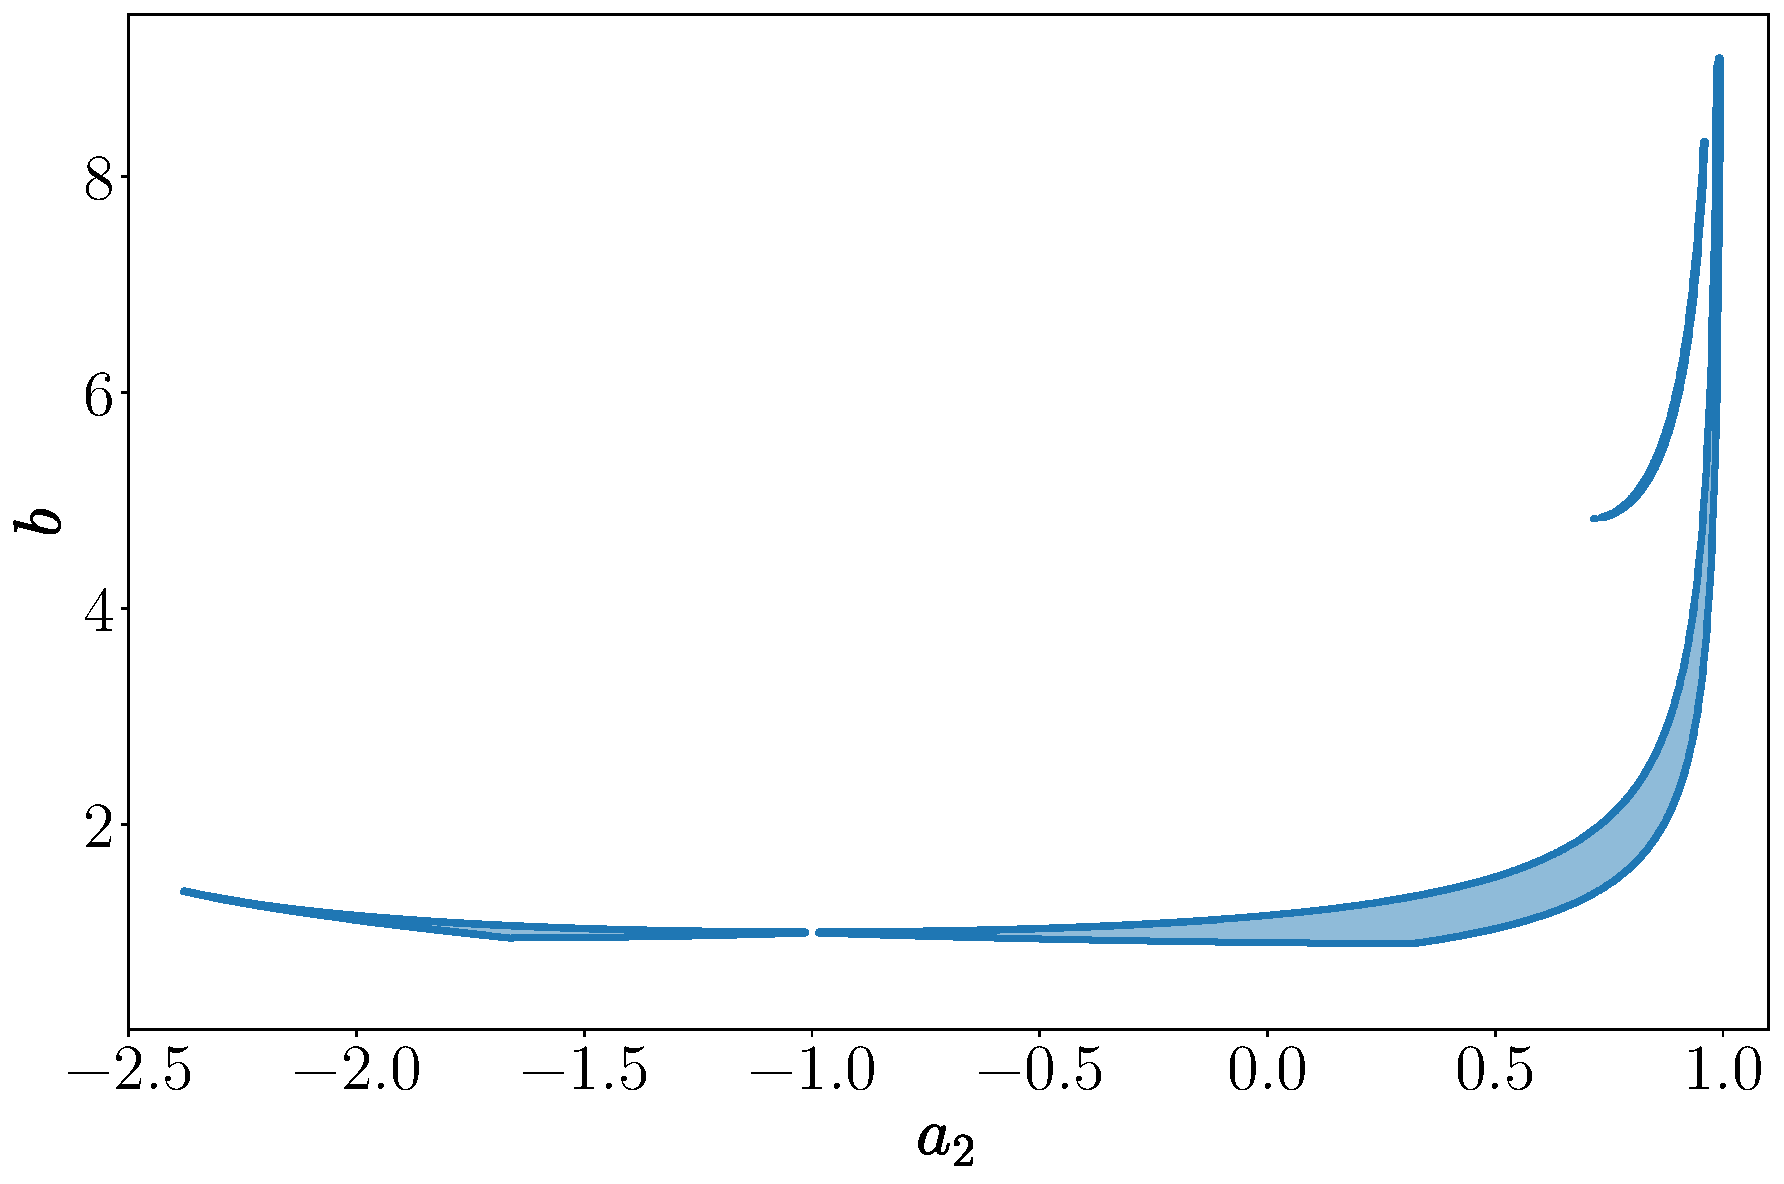
\includegraphics[scale = 0.22]{img/penrose_binaries/cmmr_joined_ergo/joined_ergo_2_a1_1.0_q_1.0.pdf}
    \label{ch:penrose_binaries/fig:ergo_joined_2_b}
  }
  \newline
  \subfloat[$a_1=1.5$, $q=0.5$]{
    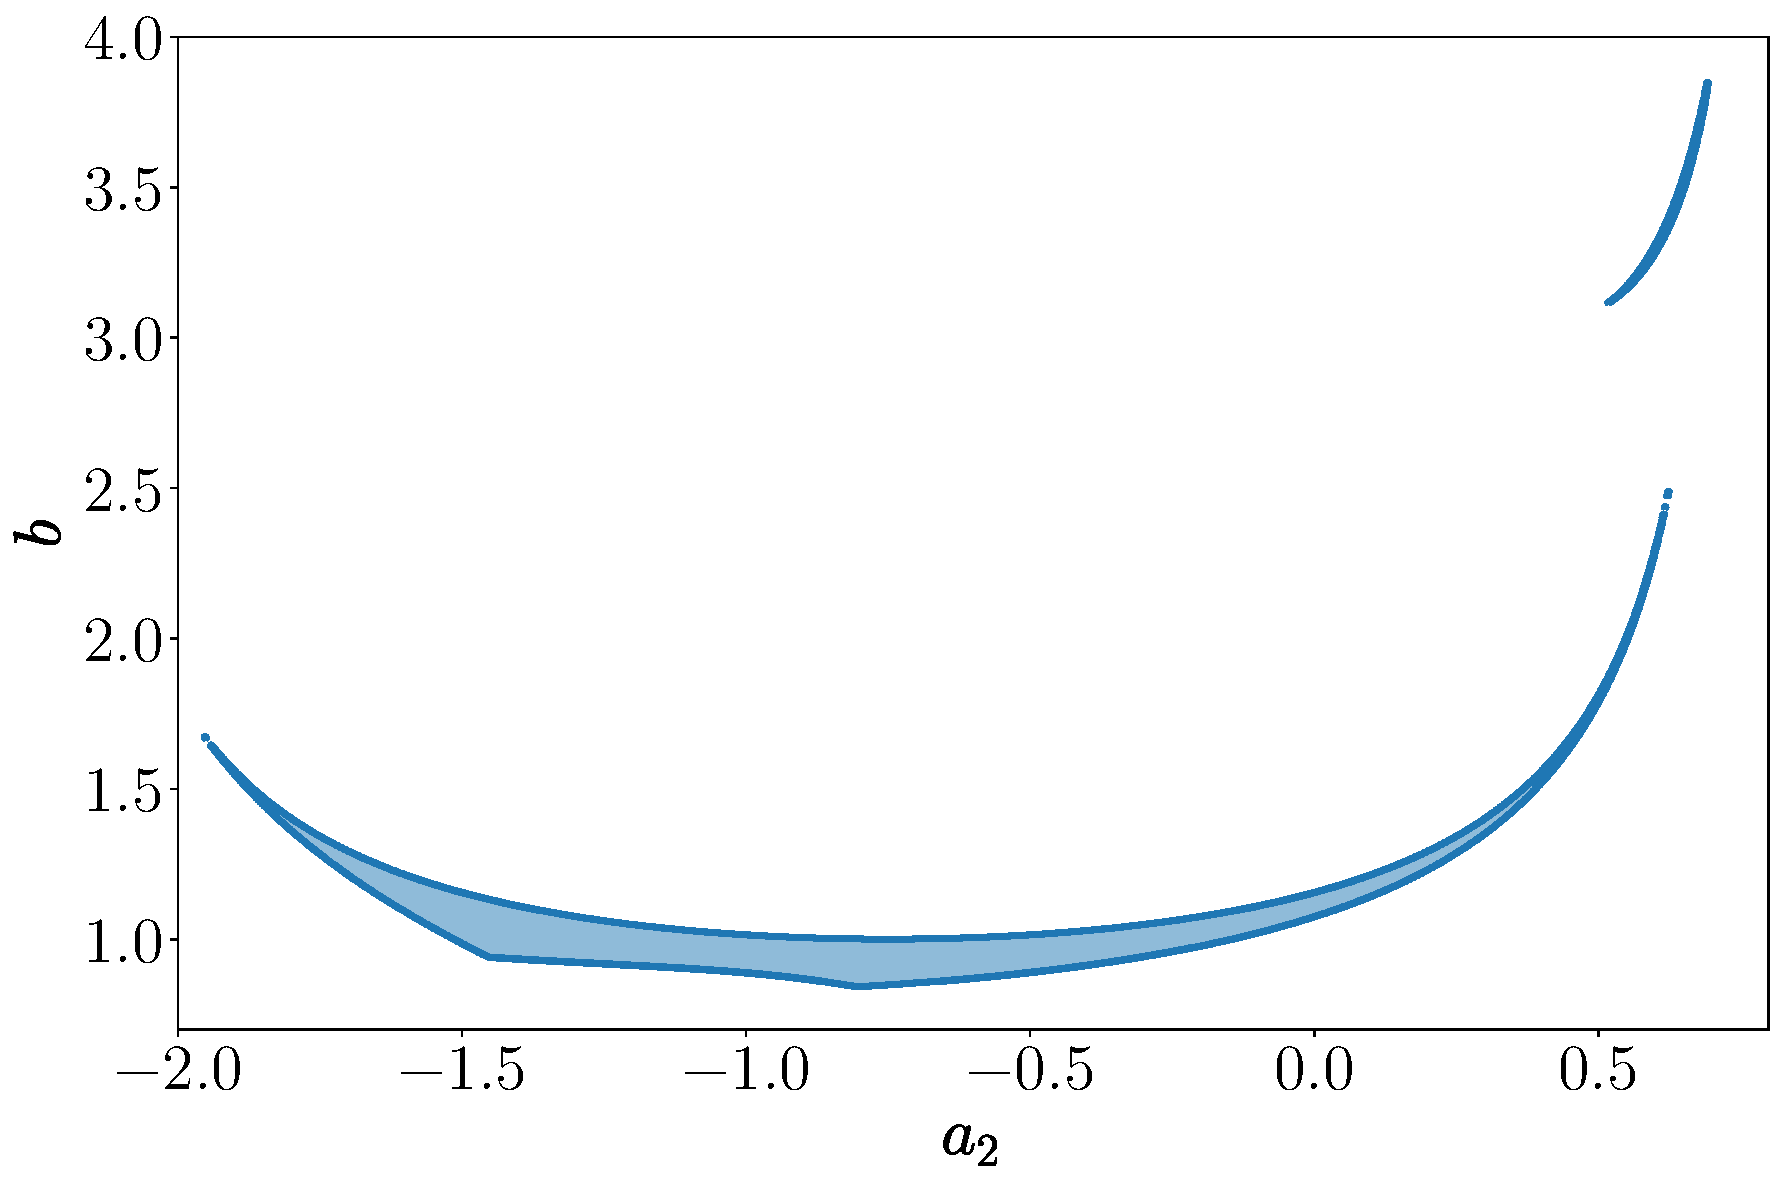
\includegraphics[scale = 0.22]{img/penrose_binaries/cmmr_joined_ergo/joined_ergo_2_a1_1.5_q_0.5.pdf}
    \label{ch:penrose_binaries/fig:ergo_joined_2_c}
  }
  \subfloat[$a_1=1.5$, $q=1.0$]{
    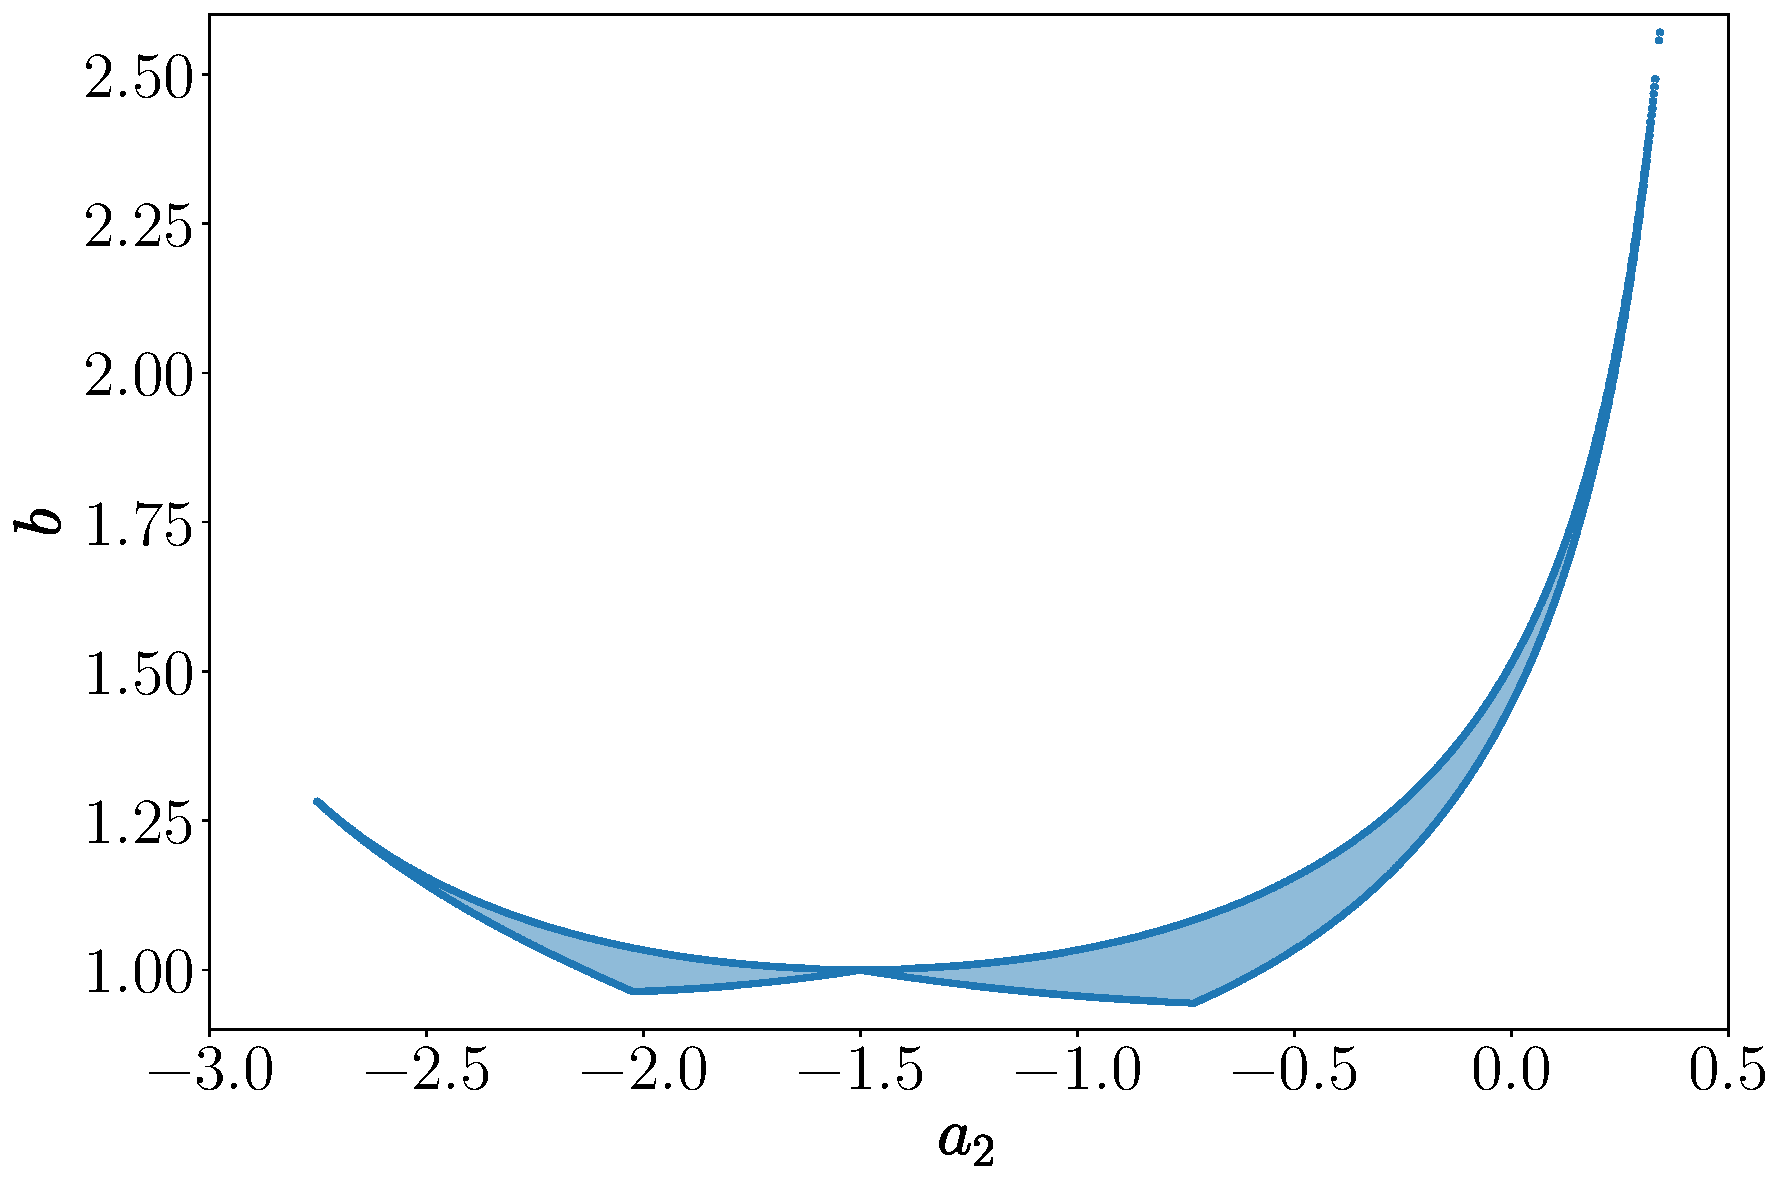
\includegraphics[scale = 0.22]{img/penrose_binaries/cmmr_joined_ergo/joined_ergo_2_a1_1.5_q_1.0.pdf}
    \label{ch:penrose_binaries/fig:ergo_joined_2_d}
  }
  \caption{Parameter spaces that allow for a common ergosphere. The blue regions represent pairs of $b$ and $a_2$ values that produce an ergosphere around both black holes for each $(a_1,q)$ indicated value.}
  \label{ch:penrose_binaries/fig:ergo_joined_2}
\end{figure}

\subsection{Geodesic motion in the $z=0$ plane}

We will make use of the Lagrangian formalism to determine the form of the geodesic equations and the motion's conserved quantities. Letting a dot represent derivatives with respect to the proper time we can write the Lagrangian of the geodesic motion as~\cite{CARROLL}
%
\begin{equation}
  2\mathcal{L} = -f(\dot{t} - \omega\dot{\varphi})^2 +f^{-1}\left[e^{2\gamma}\left( \dot{\rho}^2 + \dot{z}^2 \right) + \rho^2\dot{\varphi}^2 \right].
  \label{ch:penrose_binaries/eq:lagrangian}
\end{equation}

From \myref{ch:penrose_binaries/eq:lagrangian} we can identify two constants of the motion, the energy per unit mass as measured by a static observer at infinity $E$, given by
%
\begin{equation}
  E = f\dot{t} - \omega f\dot{\varphi}
  \label{ch:penrose_binaries/eq:energy_t_phi}
\end{equation}
%
and the angular momentum about the $z$ axis per unit mass as measured by a static observer at infinity $L$, given by
%
\begin{equation}
  L = \omega f \dot{t} + \left( \frac{\rho^2}{f} - \omega^2 f \right)\dot{\varphi}.
  \label{ch:penrose_binaries/eq:ang_mom_t_phi}
\end{equation}

We can use Eqs.~\eqref{ch:penrose_binaries/eq:energy_t_phi} and \eqref{ch:penrose_binaries/eq:ang_mom_t_phi} to find $\dot{t}$ and $\dot{\varphi}$, in terms of $E$ and $L$ which yield
%
\begin{equation}
  \dot{t} = \frac{E}{f} + \frac{\omega f (L - E\omega)}{\rho^2}
  \label{ch:penrose_binaries/eq:t_dot}
\end{equation}
%
and
%
\begin{equation}
  \dot{\varphi} = \frac{f (L - E\omega)}{\rho^2}
  \label{ch:penrose_binaries/eq:phi_dot}
\end{equation}

A third conserved quantity is the normalization of the four velocity for a massive particle, that is, $\mtrtens{\mu}{\nu}\dot{x}^\mu\dot{x}^\nu = -1$ which can be combined with Eqs.~\eqref{ch:penrose_binaries/eq:t_dot} and \eqref{ch:penrose_binaries/eq:phi_dot} to produce an expression for the particle's energy in terms of its ``spatial'' four velocities ($\dot{\rho}$ and $\dot{z}$) and it's angular momentum $L$, yielding
%
\begin{multline}
  E = \frac{-f^2\omega L}{\rho^2-\omega^2 f^2} + \left[ \frac{\rho^2e^{2\gamma}(\dot{\rho}^2 + \dot{z}^2)}{\rho^2 - \omega^2f^2} + \left( \frac{\rho fL}{\rho^2 - \omega^2f^2} \right)^2 \right. \\
  \left. + \frac{\rho^2f}{\rho^2 - \omega^2f^2} \right]^{1/2}
  \label{ch:penrose_binaries/eq:energy_rho_z}
\end{multline}
%
where the positive sign is chosen for the square root to guarantee that a static particle at infinity has positive energy.

By inverting Eq.~\eqref{ch:penrose_binaries/eq:energy_rho_z} to obtain $\dot{\rho}^2 + \dot{z}^2$ we are motivated to define the effective potential
%
\begin{equation}
  V_{\text{eff}} = \frac{\rho^2 - \omega^2 f^2}{\rho^2 e^{2\gamma}}\left[ \left( \frac{\rho fL}{\rho^2 - \omega^2f^2} \right)^2 + \frac{\rho^2f}{\rho^2 - \omega^2f^2}\right]
  \label{ch:penrose_binaries/eq:effective_potential}
\end{equation}
%
and the effective energy
%
\begin{equation}
  E_{\text{eff}} = \frac{\rho^2 - \omega^2 f^2}{\rho^2 e^{2\gamma}}\left(E + \frac{f^2\omega L}{\rho^2-\omega^2 f^2}\right)^2
  \label{ch:penrose_binaries/eq:effective_energy}
\end{equation}
%
and therefore we can write
%
\begin{equation}
  \dot{\rho}^2 + \dot{z}^2 = E_{\text{eff}} - V_{\text{eff}}.
  \label{ch:penrose_binaries/eq:effective_potential_motion}
\end{equation}

Finally, the geodesic equations can be derived using the Euler-Lagrange equations for the Lagrangian of Eq.~\eqref{ch:penrose_binaries/eq:lagrangian} and $\dot{t}$ and $\dot{\varphi}$ can be replaced with Eqs.~\eqref{ch:penrose_binaries/eq:t_dot} and \eqref{ch:penrose_binaries/eq:phi_dot}, respectively. While studying geodesic motion in binary system of two identical Kerr-Newman black holes held by a massless strut (a solution with the same general line element as Eq.~\eqref{ch:penrose_binaries/eq:line_element}) the authors of Ref.~\cite{Dubeibe2016} in Eqs.~(16) and (17) derive the explicit form of the geodesic equations for $\rho$ and $z$ in terms of $E$, $L$ and the metric functions $f$, $\omega$ and $e^{2\gamma}$ and thus we shall not repeat this information here. In our work, whenever was necessary to solve the geodesic equations numerically we implemented Eqs.~(16) and (17) of Ref.~\cite{Dubeibe2016} directly, changing only the metric functions to those described in  Sec.~IV of Ref.~\cite{MANKO2020}.

If the motion is constrained to the $z=0$ symmetry plane, we can easily determine the general characteristics of massive particle geodesics by plotting the effective potential, Eq.~\eqref{ch:penrose_binaries/eq:effective_potential}, as was done in Fig.~\ref{ch:penrose_binaries/fig:effective_potential}. The different curves represent different values of angular momenta, specifically $L = 18$ in the black curve, $L = 13$ in the red curve, $L=10$ in the blue curve and $L=4$ in the green curve. We can see that both stable and unstable circular orbits are possible, as well as escaping orbits and non-circular bounded orbits that become ``wider'' as the value of $L$ decreases.

\begin{figure}
  \centering
  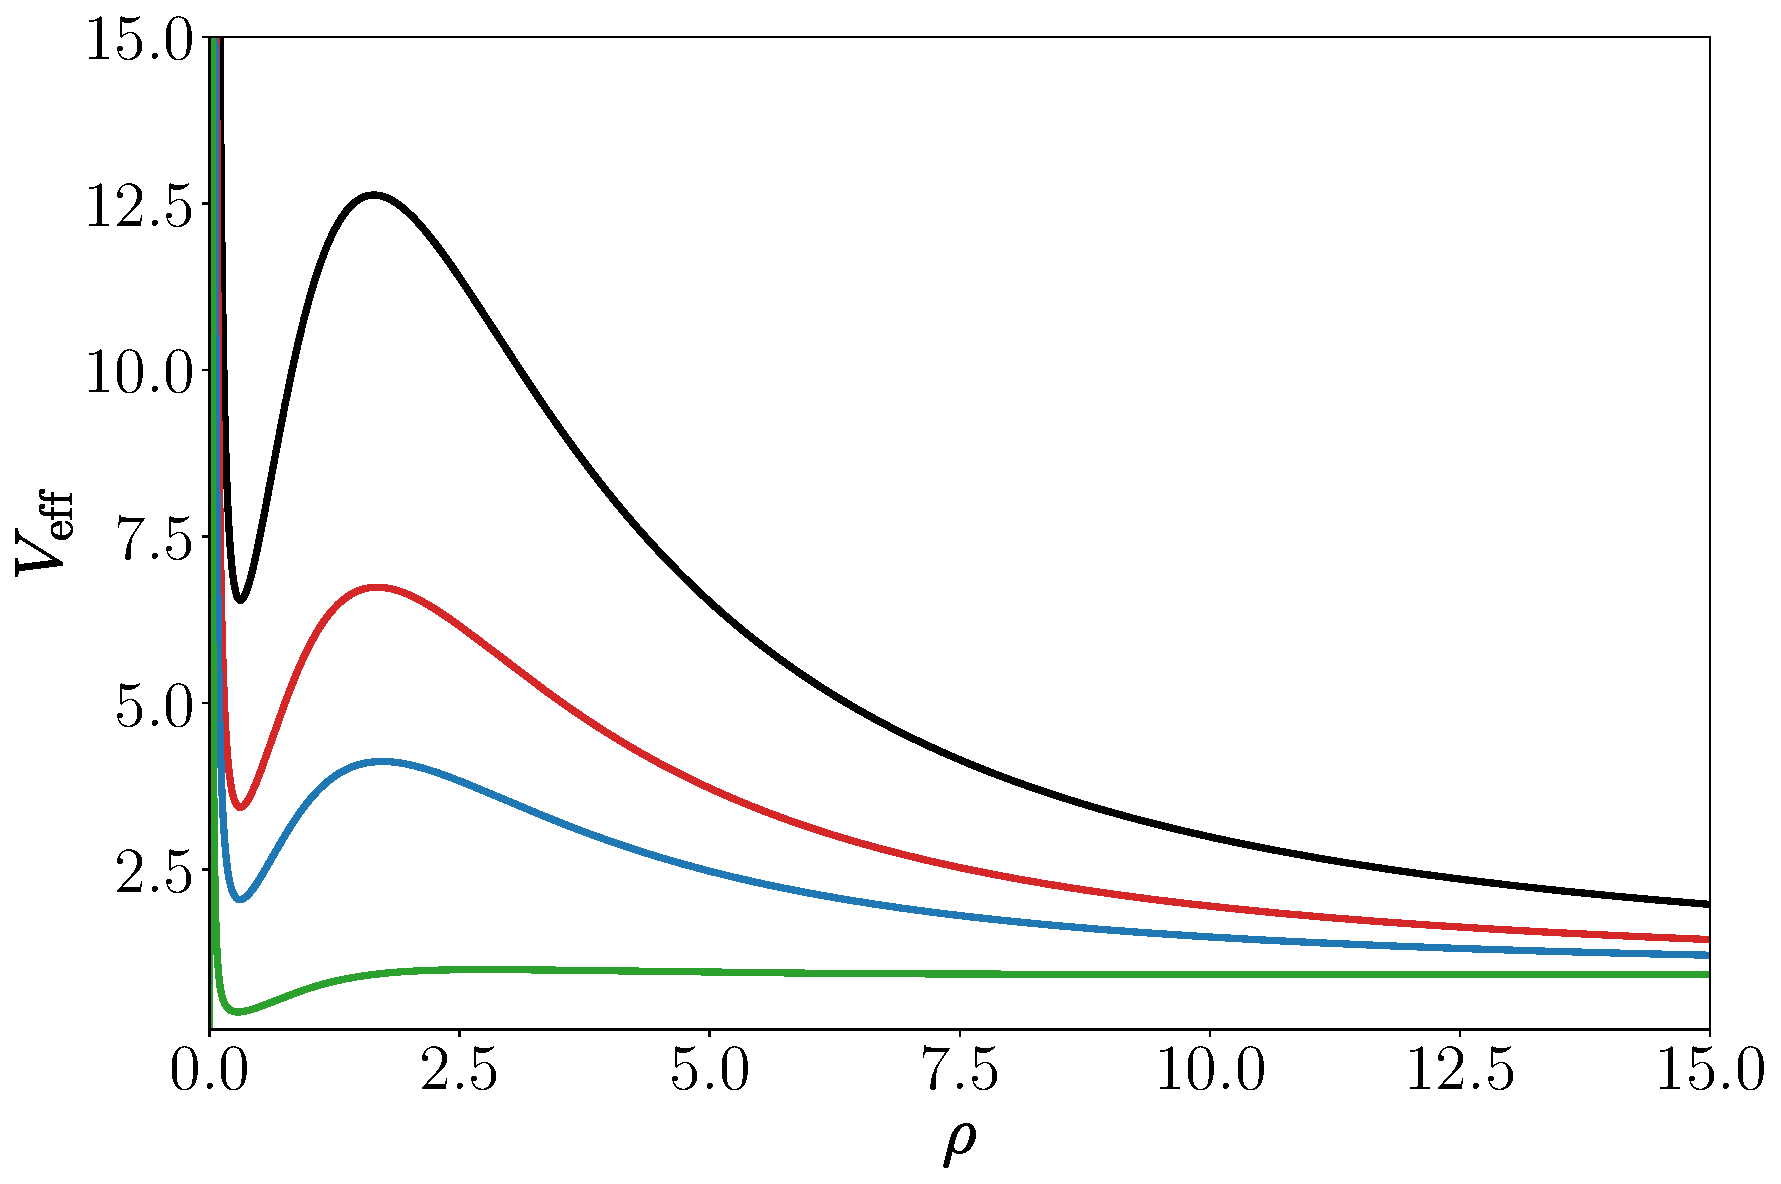
\includegraphics[scale = 0.3]{img/penrose_binaries/cmmr_vEff.pdf}
  \caption{Effective potential in the $z=0$ plane for $L=18,13,10$ and $4$ (black, red, blue and green curves respectively).}
  \label{ch:penrose_binaries/fig:effective_potential}
\end{figure}

\subsection{Negative energy orbits}

Now we turn our attention to the conditions required for a orbit to have negative energy for a static observer at infinity, as this is a necessary condition for the occurrence of the Penrose process. By inspecting Eq.~\eqref{ch:penrose_binaries/eq:energy_rho_z} we can immediately conclude that since the term in the square root is always positive, a necessary (but not sufficient) condition for the particle's energy to be negative is that
%
\begin{equation}
  \frac{-f^2\omega L}{\rho^2 - \omega^2 f^2} < 0.
  \label{ch:penrose_binaries/eq:necessary_condition}
\end{equation}
%
Multiplying both sides by the denominator we conclude that the numerator must be negative. Because $-f^2$ is always negative, the necessary condition for the existence of negative energy orbits is that
%
\begin{equation}
  (\omega < 0 \land L > 0) \lor (\omega > 0 \land L < 0)
\end{equation}
%
which simply means that the horizons must rotate in the opposite direction of the particles own rotation.

Despite $\omega(\rho,z)$ being know analytically, it's complexity does not allow us to easily reason about it's behaviour and thus we proceeded to visualize it numerically employing the same projection scheme in the Cartesian plane as was done in the visualisation of the ergosphere. With that we obtain Fig.~\ref{ch:penrose_binaries/fig:omega_value_regions}. The color indicates the value of $\omega$ at each point $(x,y)$ and the values that were graphed were deliberately chosen to lie in the range $-25 \leq \omega \leq 25$ in order to facilitate the visualization. In all panels we choose $b=0.98$ and $q=1.0$. The upper left panel shows a configuration with aligned spins $a_1=a_2=0.65$ and the upper right shows the equivalent configuration with anti-aligned spins $-a_1=a_2=0.65$. The lower row shows binaries with anti-aligned but very different spins with $a_1=0.65$ and $a_2=-0.1$ in the left panel and $a_1=-0.65$ and $a_2 = 0.1$ in the right panel. In all cases the green curve marks the boundary of the ergosphere and the black lines mark the event horizons.

From Fig.~\ref{ch:penrose_binaries/fig:omega_value_regions} it becomes clear that in the case of a system with aligned or anti aligned but very different spins one can extract energy from either of the two black holes by setting the sign of $L$ to be opposite to that of $\omega$ inside the ergosphere. The black hole that will ultimately loose part of it's energy can then only be determined uniquely from the other dynamical parameters of the particle's trajectory. In the case of anti-aligned but equal or similar spins the sign of $L$ determines uniquely which black hole can be used for energy extraction, which will be either the upper or lower black hole, depending on the sign configurations of $\omega$ and $L$ inside the ergosphere. This feature is completely compatible with the notion that energy can only be extracted inside the ergospehre. For spin configurations in which a single ergosphere exists around both black holes, energy can be extracted from either hole while in configurations in which the ergospheres are located around each hole but are disconnected, energy can be extracted from only one of the constituents.

\begin{figure}
  \centering
  \subfloat[$a_1 = a_2 = 0.65$]{
    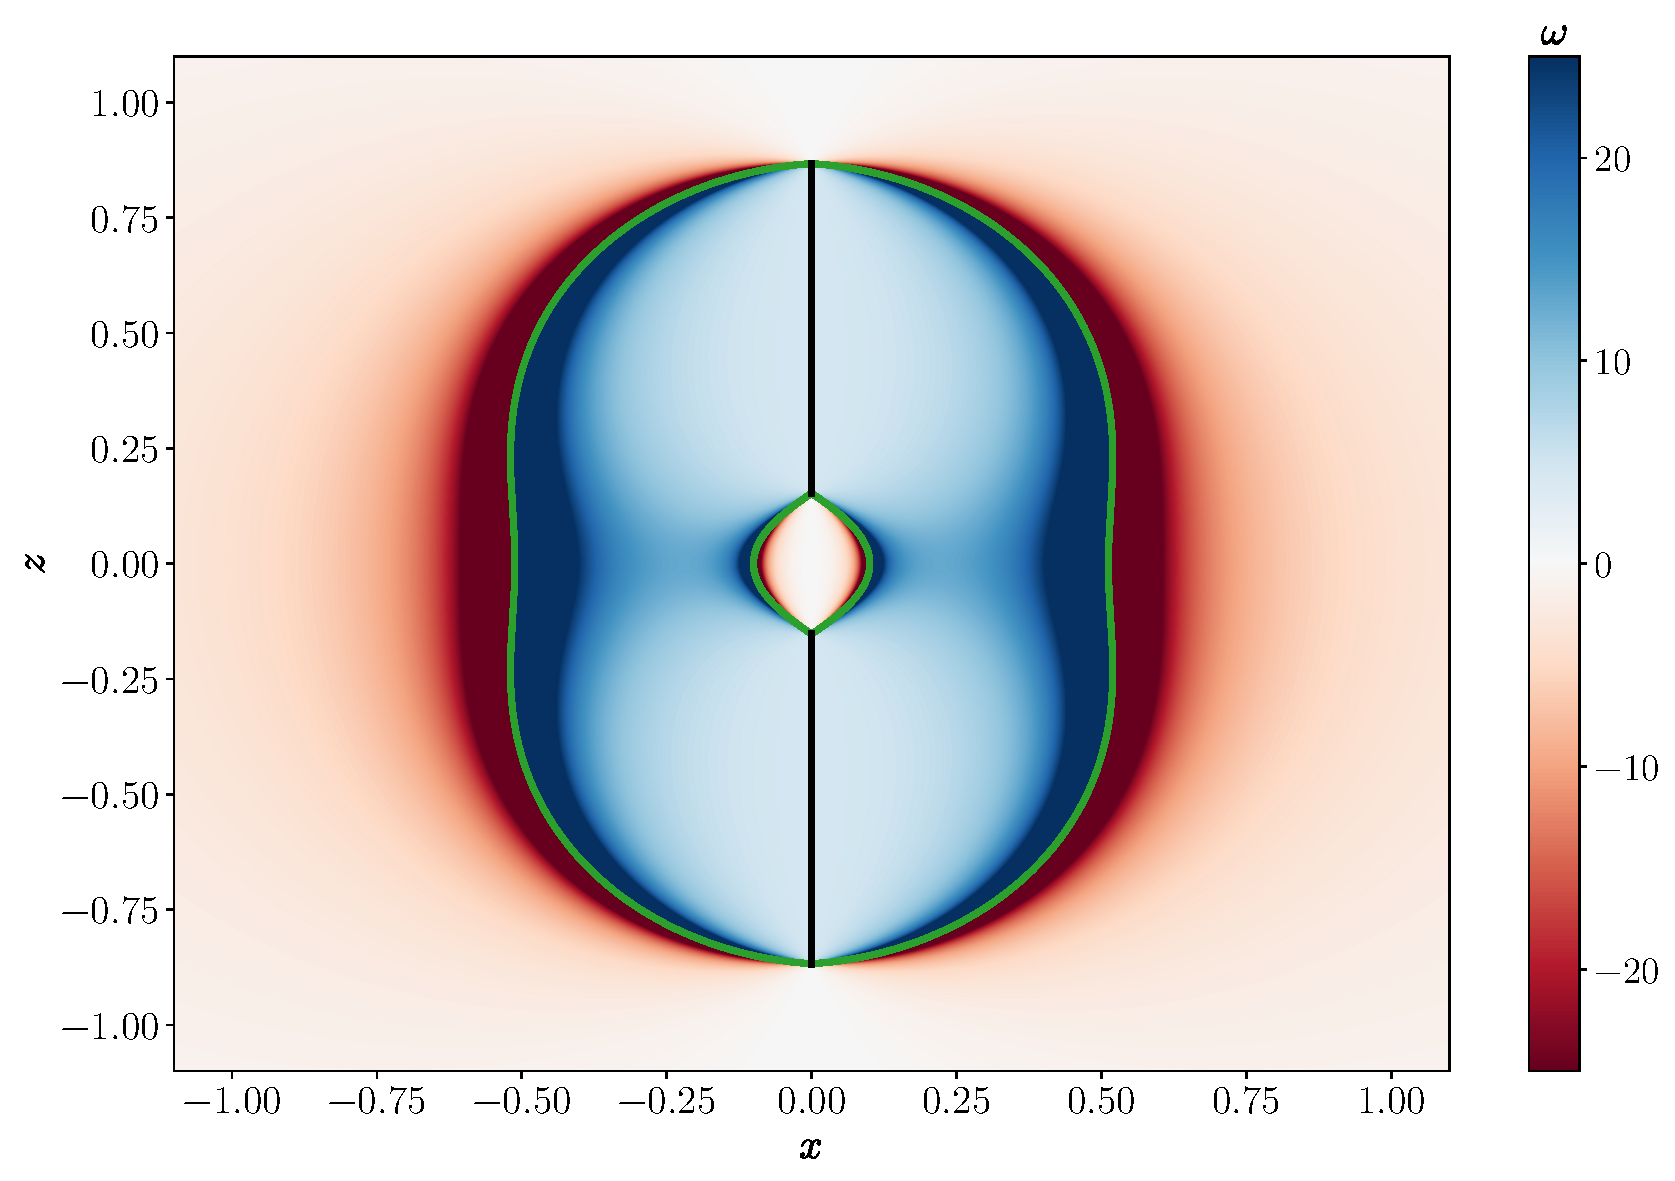
\includegraphics[scale = 0.25]{img/penrose_binaries/cmmr_omega/omega_b_0.98_q_1.0_a1_0.65_a2_0.65.pdf}
    \label{ch:penrose_binaries/fig:omega_dens_a}
  }
  \subfloat[$a_1= -a_2 = -0.65$]{
    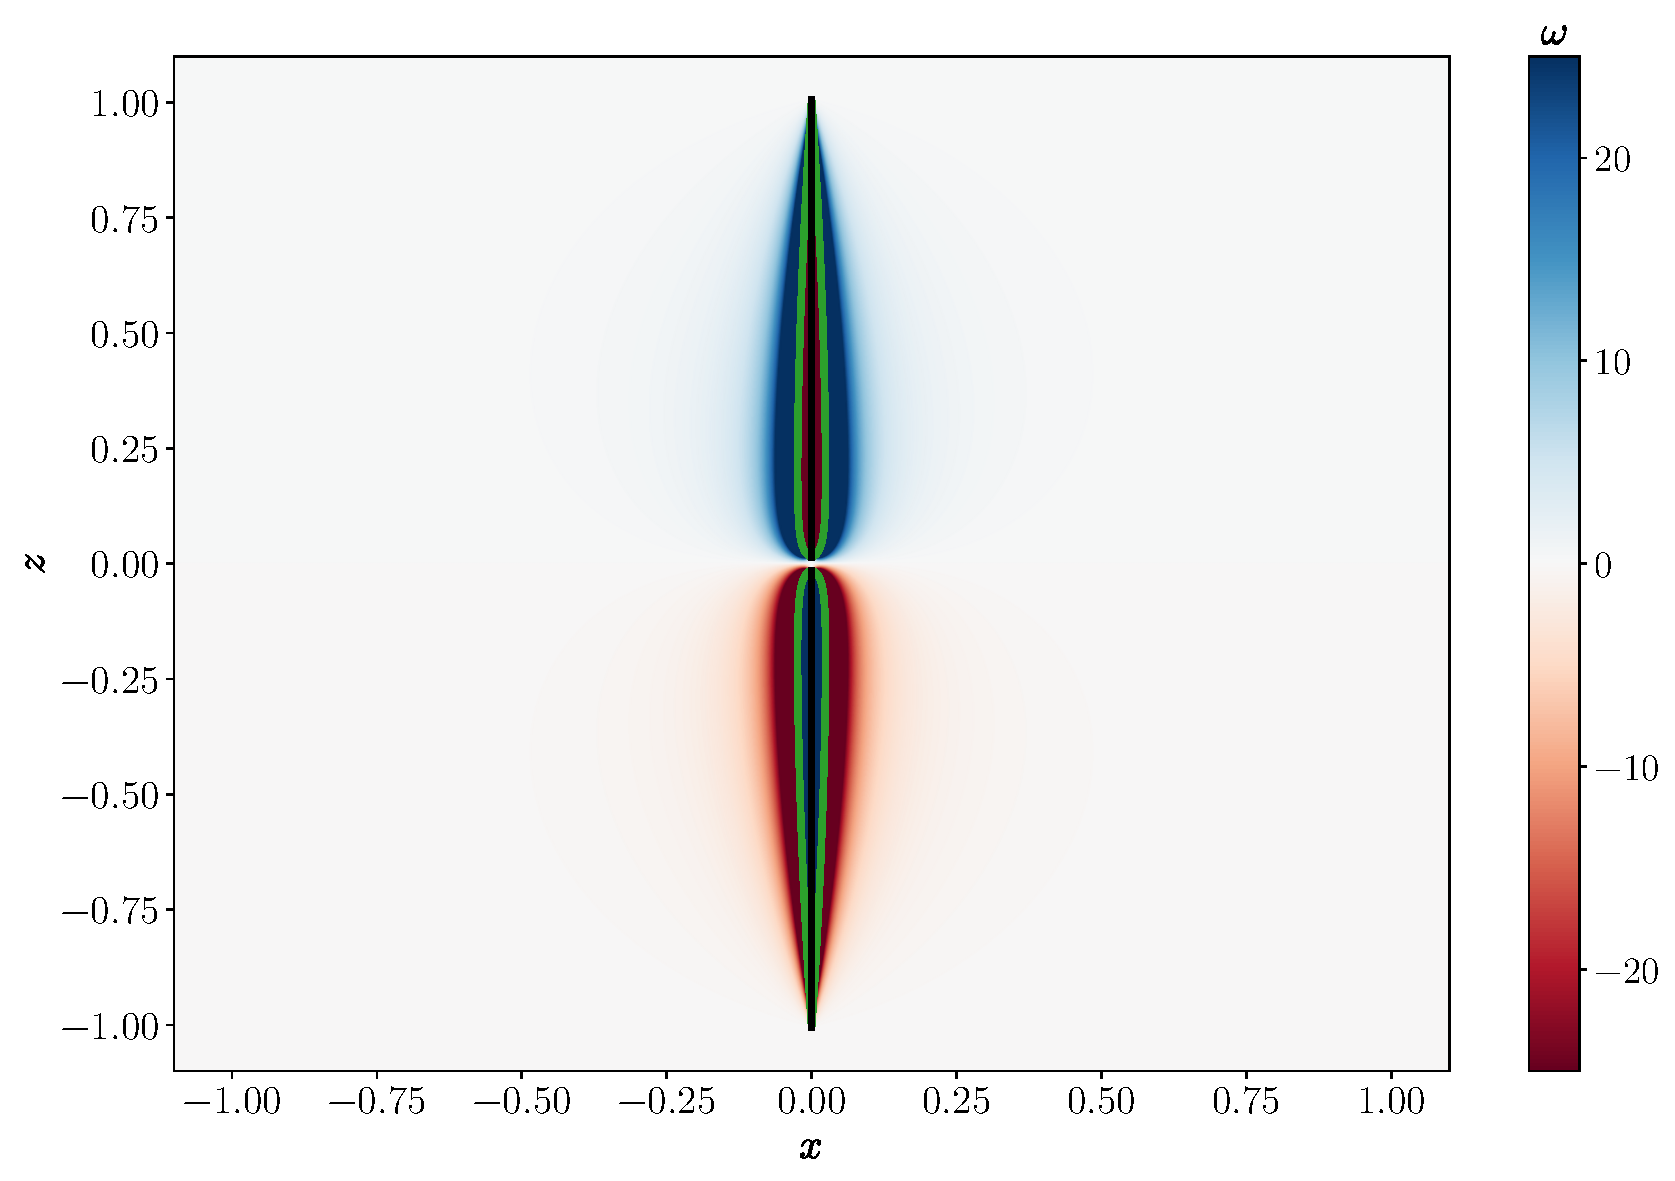
\includegraphics[scale = 0.25]{img/penrose_binaries/cmmr_omega/omega_b_0.98_q_1.0_a1_-0.65_a2_0.65.pdf}
    \label{ch:penrose_binaries/fig:omega_dens_b}
  }
  \newline
  \subfloat[$a_1= 0.65$, $a_2 = -0.1$]{
    \includegraphics[scale = 0.25]{img/penrose_binaries/cmmr_omega/omega_b_0.98_q_1.0_a1_0.65_a2_-0.1.pdf}
    \label{ch:penrose_binaries/fig:omega_dens_c}
  }
  \subfloat[$a_1= -0.65$, $a_2 = 0.1$]{
    \includegraphics[scale = 0.25]{img/penrose_binaries/cmmr_omega/omega_b_0.98_q_1.0_a1_-0.65_a2_0.1.pdf}
    \label{ch:penrose_binaries/fig:omega_dens_d}
  }
  \caption{The value of $\omega(\rho,z)$ projected in Cartesian coordinates. In all plots $b=0.95$ and $q=1.0$. The green curve marks the limit of the ergospehre and the black lines mark the event horizons.}
  \label{ch:penrose_binaries/fig:omega_value_regions}
\end{figure}

\subsection{Efficiency of energy extraction}

We now turn our attention to the maximum energy that can be extracted from the system by means of the Penrose process. It widely know that no more energy can be extracted than the \textit{irreducible mass} of each black hole~\cite{RUFFINI1971,CHRISTODOULOU1970,CARROLL}. The irreducible mass $M_{\text{irr}}$ is related to the horizon area $A$ by the well know formula~\cite{CARROLL}
%
\begin{equation}
  M_{\text{irr}} = \sqrt{\frac{A}{16\pi}}.
  \label{ch:penrose_binaries/eq:irreducible_mass}
\end{equation}
%
The entropies of each black hole in the CMMR metric are know and given in Eq.~(22) of Ref.~\cite{MANKO2020}. Given that the entropy $S$ and horizon area are related by $A=4S$ we have that the maximum energy that can be extracted from the system is the sum of the maximum energy that can be extracted from each hole individually, that is
%
\begin{equation}
  E_{\text{max}} = \left(m_1 - \sqrt{\frac{S_1}{4\pi}}\right) + \left(m_2 - \sqrt{\frac{S_2}{4\pi}}\right).
  \label{ch:penrose_binaries/eq:max_extract_energy}
\end{equation}

In the traditional Penrose process there is only one particle of negative energy and thus only one of the black holes will loose part of it's rotation. In practice this meas that only one of the terms inside the parenthesis of Eq.~\ref{ch:penrose_binaries/eq:max_extract_energy} will contribute to the energy extraction. A remarkable fact is that if one takes the limit of $R \rightarrow \infty$ of one of these terms (e.g. the first) in Eq.~\ref{ch:penrose_binaries/eq:max_extract_energy} one obtains
%
\begin{equation}
  E_{\text{max}} = m_1 - \frac{1}{\sqrt{2}}\left(m_1^2 + \sqrt{m_1^4 - j_1^2}\right)^{1/2}
  \label{ch:penrose_binaries/eq:energy_extraction_kerr_limit}
\end{equation}
%
where we remind that $j_1=a_1m_1$. This expression is exactly the one obtained for the maximum extracted energy in the case of a single Kerr black hole of mass $m_1$ and angular momentum $j_1$~\cite{CARROLL} which reassures us to the fact that a Kerr binary behaves as a system of isolated Kerr black holes if their separation is large.

\section{Geodesic motion in arbitrary space-times}

In this section we will discuss a method that we intend to implement which would allow us to investigate the Penrose process in arbitrary (even numerically evolved) spacetimes. As we've seen, the Penrose mechanism depends on the existence of orbits that have negative energy according to a static observer far away from the system. If such orbits exist, energy can be extracted from the system. We've also shown that such orbits must lie inside the ergosphere of the binary system, but the notion of ergosphere is not easily generalized to dynamic space-times and remains an open problem. Instead of attempting to define an ergosphere in a dynamical background, we will investigate geodesic motion in such background. The methods and tools for this are already well know in the branch of \emph{ray tracing} in NR for computing the shadows of binary black holes. It all hinges on the ADM (Arnowitt, Deser and Misner) of the geodesic equation.

\subsection{ADM Decomposition of the geodesic equation}

The ADM decomposition, also know as the $3+1$ decomposition is a formulation of GR that rewrite Einstein's field equations as a Cauchy (initial value) problem and is a very common representation of spacetimes used in NR. In this decomposition, the spacetime metric is written as~\cite{BAUMGARTE}

\begin{equation}
  \ud s^2 = -\alpha^2 \ud t^2 + \tens{\gamma}{}{ij} \left( \ud \tens{x}{i}{} + \tens{\beta}{i}{}\ud t\right) \left( \ud \tens{x}{j}{} + \tens{\beta}{j}{}\ud t\right)
  \label{ch:penrose_binaries/eq:adm_metric}
\end{equation}
%
where $\alpha$ is the lapse function, $\tens{\beta}{i}{}$ the shift vector and $\tens{\gamma}{}{ij}$ the spatial metric.

The decomposition of the geodesic equation we will adopt follows Ref.~\cite{BOHN2015} closely. We note that a very similar approach was also develop in Ref.~\cite{VINCENT2012}, which we also refer for additional details. We start by defining the auxiliary variable

\begin{equation}
  \tens{\Pi}{}{i} \equiv \frac{\tens{p}{}{i}}{\alpha \tens{p}{}{0}} = \frac{\tens{p}{}{i}}{\sqrt{\tens{\gamma}{jk}{} \tens{p}{}{j} \tens{p}{}{k}}}
  \label{ch:penrose_binaries/eq:big_pi_def}
\end{equation}
%
where $p^i \equiv \ud x^{i}/\ud \tau$ is the particle's 4-momentum, $x^i$ the spacetime coordinates and $\tau$ the particle's proper time.

Using the ADM decomposition, the geodesic equation can be written as~\cite{BOHN2015}

\begin{align}
  \der{\tens{\Pi}{}{i}}{t} =          & -\indexdel{i}\alpha + \left[ \left( \indexdel{j}\alpha \right) \tens{\Pi}{j}{} - \alpha \tens{K}{}{jk} \tens{\Pi}{j}{} \tens{\Pi}{k}{}\right]\tens{\Pi}{}{i} + \left( \indexdel{i}\tens{\beta}{k}{} \right) \tens{\Pi}{}{k} - \frac{1}{2} \alpha \left( \indexdel{i} \tens{\gamma}{jk}{} \right) \tens{\Pi}{}{j} \tens{\Pi}{}{k} \\
  \der{\tens{x}{i}{}}{t} =            & \alpha \tens{\Pi}{i}{} - \tens{\beta}{i}{}                                                                                                                                                                                                                                                                                       \\
  \der{\ln(\alpha\tens{p}{0}{})}{t} = & -\left( \indexdel{i} \alpha \right) \tens{\Pi}{i}{} + \alpha \tens{K}{}{ij}\tens{\Pi}{i}{}\tens{\Pi}{j}{}
  \label{ch:penrose_binaries/eq:adm_geodesic_eq}
\end{align}
%
where $t$ is the coordinate time, $\tens{K}{}{ij}$ is the extrinsic curvature and $\tens{\Pi}{i}{} = \tens{\gamma}{ij}{}\tens{\Pi}{}{j}$.
\subsection{Observed quantities}
\subsection{Proposal for investigating the Penrose process in numeric space-times}
